\documentclass[11pt]{report}

\usepackage[margin=1.2in]{geometry}

\usepackage{verbatim} 

\usepackage{graphicx}

\usepackage{amsmath}

\usepackage{fancyhdr}

\usepackage{titlesec}

\usepackage{float}

\usepackage{tabularx,ragged2e,booktabs,caption}

\usepackage{xspace}

\usepackage{algorithm}

\usepackage{algorithmicx}

\usepackage{tocloft}

\usepackage{longtable} 

\usepackage{enumitem}

\usepackage{algpseudocode}

\usepackage{setspace}  

\usepackage{microtype}

\usepackage[colorlinks=true,linkcolor=black]{hyperref} 

\usepackage{pdfpages}

\usepackage{url}

\usepackage{pgfplots}

\usepackage{tikz}

\usetikzlibrary{shapes.geometric, arrows, positioning, calc}

\pgfplotsset{compat=1.18}

\tolerance=1000

\emergencystretch=1em

\begin{document}

\renewcommand\bibname{References}

\pagestyle{fancy}

\fancyhead{}

\fancyfoot{}

\fancyfoot[c]{\thepage}

\fancyfoot[l]{CSD 416 - Project Phase 2 2024-25}

\renewcommand{\chaptermark}[1]{\markboth{\thechapter.\ #1}{}}

\renewcommand{\headrulewidth}{0.1pt}

\addtolength{\headheight}{\baselineskip}

\fancyhead[L]{\slshape \nouppercase{\leftmark}}

\fancyhead[R]{\thepage}

\bibliographystyle{plain}

%% ====================== TITLE PAGE ======================

\thispagestyle{empty}

\begin{center}

\vspace*{2cm}

{\LARGE \textbf{Edge-Driven Semi-Autonomous EV Charging Station Using Quantized Vision Models and Real-Time License Plate Recognition}} \\[0.3cm]

{\large \textbf{CSD416 Project Phase II Report}} \\

\vspace{2cm}

\renewcommand{\arraystretch}{1.3}

\begin{tabular}{ll}

MDL22CSBS026 & Izz Al Din Noufel Mukthar \\

MDL22CSBS029 & Joel K George \\

MDL22CSBS050 & Sarah Ann Pothen \\

MDL22CSBS053 & Shahma Fathima \\

\end{tabular}

\vspace{1.5cm}

{\large B. Tech Computer Science \& Engineering} \\

\vspace{2cm}


\includegraphics[width=0.25\textwidth]{logo.jpg} \\[0.5cm]

\textbf{Department of Computer Engineering} \\

Model Engineering College \\

Thrikkakara, Kochi 682021 \\

Phone: +91-484-2575370 \\

\texttt{http://www.mec.ac.in} \\

\texttt{hodcs@mec.ac.in} \\

\vfill

{\large April 2026}

\end{center}
%% ====================== CERTIFICATE ======================
\clearpage
\thispagestyle{empty}

\begin{center}
{\Large \textbf{Model Engineering College, Thrikkakara}}\\[0.2cm]
{\large \textbf{Department of Computer Engineering}}\\[0.6cm]


\includegraphics[width=0.15\textwidth]{logo.jpg}\\[0.4cm]

{\Large \textbf{C E R T I F I C A T E}}\\
\end{center}

\vspace{0.3cm}

\noindent
This is to certify that this report titled 
\textbf{Edge-Driven Semi-Autonomous EV Charging Station Using Quantized Vision Models and Real-Time License Plate Recognition} 
is a bonafide record of the work done by

\vspace{0.3cm}

\begin{center}
\renewcommand{\arraystretch}{1.3}
\begin{tabular}{ll}
MDL22CSBS026 & Izz Al Din Noufel Mukthar \\
MDL22CSBS029 & Joel K George \\
MDL22CSBS050 & Sarah Ann Pothen \\
MDL22CSBS053 & Shahma Fathima \\
\end{tabular}
\end{center}

\vspace{0.3cm}

\noindent
Eighth Semester B. Tech. Computer Science \& Engineering students, for the course work in \textbf{CSD416 Project Phase II}, which is the second part of the two-semester project work, under our guidance and supervision, in partial fulfillment of the requirements for the award of the degree, \textbf{B. Tech. Computer Science \& Engineering} of \textbf{APJ Abdul Kalam Technological University}.

\vspace{0.6cm}

\noindent
\begin{minipage}[t]{0.48\textwidth}
\vspace{0pt}
\raggedright

\textbf{Guide}\\
Dr. Manju K\\
Associate Professor\\
Department of Computer Engineering\\[1.2cm]

\textbf{Coordinator}\\
Chinju P Varghese\\
Assistant Professor\\
Department of Computer Engineering\\[0.8cm]

April, 2026

\end{minipage}
\hfill
\begin{minipage}[t]{0.48\textwidth}
\vspace{0pt}
\raggedleft

\textbf{Head of the Department}\\
Dr. Binu V. P.\\
Professor\\
Department of Computer Engineering\\[1.2cm]

\end{minipage}

%% ====================== ACKNOWLEDGEMENTS ======================
\clearpage
\pagenumbering{roman}
\thispagestyle{empty}

\begin{center}
\textbf{\LARGE Acknowledgements}
\end{center}

\vspace{0.8cm}

This project would not have been possible without the kind support and help of many individuals.
We would like to extend our sincere thanks to all of them.

First of all, we would like to thank our esteemed Principal, \textbf{Prof. Dr. Jayachandran E.S.}, for his
guidance and support in maintaining a calm and refreshing environment to work in and also for
providing the facilities that this work demanded.

We are highly indebted to \textbf{Dr. Binu V.P.}, Professor and Head of the Department,
and our Project Coordinator, \textbf{Chinju P Varghese}, Assistant Professor, for their guidance,
support and constant supervision throughout the duration of the work as well as for providing all
the necessary information and facilities that this work demanded.

We would like to thank our Project Guide, \textbf{Dr. Manju K}, Associate Professor, for her support
and valuable insights and also for helping us in correcting mistakes during the course of the work.

We offer our sincere gratitude to all our friends and peers for their support and encouragement
that helped us get through the tough phases during the course of this work.

Last but not the least, we thank the Almighty God for guiding us through and enabling us to
complete the work within the specified time.

\vspace{1.5cm}

\begin{flushleft}
\textbf{Joel K George} \\
\textbf{Izz Al Din Noufel Mukthar}\\
\textbf{Sarah Ann Pothen} \\
\textbf{Shahma Fathima} 
\end{flushleft}

%% ====================== ABSTRACT ======================
\begin{abstract}
\pagenumbering{roman}
The rapid proliferation of Electric Vehicles (EVs) has exposed critical user-experience shortcomings in existing charging infrastructure, which remains heavily reliant on fragmented mobile applications, RFID cards, and cloud-dependent authentication flows. This project presents the design and implementation of an edge-computing-based semi-autonomous EV charging station that leverages real-time Automatic License Plate Recognition (ALPR) to eliminate manual user identification entirely.

A YOLOv11 object detection model, fine-tuned for license plate detection and statically quantized from 32-bit floating point (FP32) to 8-bit integer (INT8) precision using ONNX Runtime, is deployed on a Raspberry Pi 4B edge node. To resolve a critical signed INT8 operator incompatibility on ARM CPU kernels, we developed a custom ONNX graph patching script that shifts convolution weights into the unsigned UINT8 domain. The quantization reduces the model size from approximately 200\,MB to 25\,MB---an 87.5\% reduction---while achieving a 3.78$\times$ inference speedup with only a 1.2\% reduction in mAP@0.5.

Coupled with EasyOCR for character extraction, regex-validated pattern matching, and SQLite-backed vehicle database lookups, the system enables a frictionless ``park and plug'' charging experience. A native iOS application built with SwiftUI and AVFoundation streams camera frames via WebSocket and displays real-time bounding box overlays and a verification success screen upon authorization. The end-to-end pipeline achieves sub-second latency on the Raspberry Pi, demonstrating that edge-based computer vision can fundamentally transform the EV charging experience by eliminating the multi-step friction inherent in current app-centric systems.
\end{abstract}
\tableofcontents
\cleardoublepage
\addcontentsline{toc}{chapter}{\listfigurename}
\listoffigures
\newpage
\addcontentsline{toc}{chapter}{\listtablename}
\listoftables
\pagestyle{fancy}
\fancyhf{} % clear all header and footer fields

% Footer
\fancyfoot[L]{Dept. of Computer Engineering, MEC, 2026}
\fancyfoot[C]{}
\fancyfoot[R]{\thepage}
%% ========================================================
%% CHAPTER 1: INTRODUCTION
%% ========================================================
\chapter{Introduction}
\pagenumbering{arabic}
\label{intro}

\section{Proposed Project}
\subsection{\label{gn}General Background}

The global transition towards sustainable transportation has driven unprecedented growth in Electric Vehicle (EV) adoption. According to the International Energy Agency (IEA), global EV sales surpassed 14 million units in 2023, representing a year-over-year increase of 35\%. The cumulative number of EVs on the road worldwide crossed the 40-million mark by end of 2023, with projections indicating that EVs will constitute over 60\% of new car sales by 2030 in leading markets such as China, Europe, and North America~\cite{iea2024}. This rapid expansion places enormous pressure on the charging infrastructure to scale not only in capacity but also in usability. \par

India, in particular, has witnessed a dramatic acceleration in EV adoption. The Indian government's FAME II (Faster Adoption and Manufacturing of Electric Vehicles) scheme, combined with state-level subsidies and declining battery costs, has propelled EV sales from approximately 5,000 units in 2018 to over 1.5 million units in 2023. The government has set an ambitious target of achieving 30\% EV penetration by 2030, necessitating a corresponding expansion of the public charging network from the current 12,000 stations to an estimated 400,000 stations nationwide. \par

Despite significant hardware advances in charging technology---including Level 2 AC chargers, DC fast chargers capable of delivering 150\,kW or more, and emerging ultra-fast chargers exceeding 350\,kW---the user experience at public and semi-public EV charging stations remains a persistent friction point. The prevailing interaction model requires EV drivers to engage with operator-specific smartphone applications, downloading, registering, authenticating, and initiating sessions through multi-step digital workflows before any electricity flows~\cite{hardman2018}. \par

This friction is compounded by the fragmented nature of the charging network. Unlike the relatively standardized petrol station experience, EV drivers must navigate a patchwork of competing operators (Tata Power, ChargeZone, Ather Grid, EESL, etc.), each with their own mobile application, account system, pricing model, and payment gateway. A driver visiting five different charging networks must maintain five separate apps, five accounts, and potentially five different payment methods. \par

Edge Computing offers a compelling alternative by relocating computational intelligence from centralized cloud servers directly to the point of service~\cite{shi2016}. For EV charging, this means equipping each station with sufficient on-device processing capability to autonomously identify vehicles, verify authorization, and initiate charging sessions---all without requiring cloud round-trips or smartphone intermediaries during the critical authentication window.

\subsection{Motivation}

The motivation for this project stems from four key observations about the current EV charging ecosystem:

\begin{enumerate}
    \item \textbf{App Fatigue:} Research indicates that 67\% of EV drivers express frustration with maintaining multiple operator-specific applications~\cite{hardman2018}. The average public charging session involves 4--7 discrete interaction steps before charging begins, compared to the single ``swipe and go'' gesture at a petrol pump.
    
    \item \textbf{Connectivity Dependency:} Cloud-based authentication fails in environments with poor cellular coverage---precisely the locations where EV chargers are most needed: underground parking garages, rural highway rest stops, and basement-level commercial complexes.
    
    \item \textbf{Accessibility Gaps:} The app-centric model disproportionately excludes elderly users, tourists without local SIM cards, and individuals with limited smartphone proficiency. An autonomous, vision-based identification system eliminates this barrier entirely.
    
    \item \textbf{Edge Computing Maturity:} The convergence of affordable single-board computers (Raspberry Pi 4B at \$35--\$55), efficient quantization techniques, and optimized inference runtimes (ONNX Runtime) has made it feasible to deploy production-quality computer vision at the network edge for the first time.
\end{enumerate}

\subsection{Objective of the Project}
\textbf{Objectives}
\begin{itemize}
    \item Develop a real-time Automatic License Plate Recognition (ALPR) system deployable on resource-constrained edge hardware (Raspberry Pi 4B).
    \item Quantize a YOLOv11 object detection model from FP32 to INT8 precision for efficient edge inference, achieving $>$85\% model size reduction with $<$2\% accuracy degradation.
    \item Resolve the signed INT8 operator incompatibility on ARM CPU kernels through custom ONNX graph patching.
    \item Implement an asynchronous WebSocket-based inference server for real-time frame processing at $>$2 FPS.
    \item Build a native iOS client application for camera streaming with live detection overlays using SwiftUI and AVFoundation.
    \item Design a complete verification pipeline: plate detection $\to$ OCR $\to$ regex validation $\to$ SQLite database lookup $\to$ authorization signal.
    \item Achieve end-to-end pipeline latency under 1 second on the Raspberry Pi 4B.
\end{itemize}

\subsection{Scope of the Project}
The scope of this project encompasses the complete design, development, testing, and demonstration of an edge-based ALPR system for EV charging authorization. Specifically, the project covers:

\begin{itemize}
    \item \textbf{Model Optimization:} Fine-tuning and quantizing a YOLOv11 model for license plate detection, including the development of a custom ONNX graph patching tool for ARM compatibility.
    \item \textbf{Edge Server:} A Python-based asynchronous WebSocket server running on Raspberry Pi 4B that handles frame reception, inference, OCR, validation, and database lookup.
    \item \textbf{iOS Client:} A native SwiftUI application that streams camera frames, renders detection overlays, and displays verification results.
    \item \textbf{Database Backend:} An SQLite database for vehicle registration, owner information, and account balance management.
    \item \textbf{Documentation:} Comprehensive project documentation including this report, an IEEE-format research paper, and presentation materials.
\end{itemize}

The project explicitly excludes: physical charger hardware integration (GPIO relay control is discussed as future work), production-grade security hardening, payment gateway integration, and multi-language OCR support.

%% ========================================================
%% CHAPTER 2: PROBLEM STATEMENT AND SOLUTION
%% ========================================================
\chapter{Problem Statement and Solution}
\section{Problem Statement}
\subsection{\label{ps}Problem Statement}

Current EV charging stations require users to interact with operator-specific smartphone applications for authentication and session initiation. This multi-step process---involving app installation, account registration, QR code scanning, and payment confirmation---creates significant friction, connectivity dependencies, and accessibility barriers.

The typical charging session workflow at a public EV station involves the following steps:
\begin{enumerate}
    \item The driver arrives at the charging station and locates an available charger.
    \item The driver identifies the charging network operator from signage on the charger.
    \item If the operator's app is not installed, the driver downloads it from the App Store or Play Store.
    \item The driver creates an account (email, password, phone number, payment method).
    \item The driver opens the app, scans a QR code on the charger, or enters the station ID manually.
    \item The driver selects a charging plan and confirms payment.
    \item Charging begins after cloud-side verification.
    \item Upon completion, the driver receives a notification and the session ends.
\end{enumerate}

This 8-step process introduces multiple failure points: app crashes, poor cellular connectivity, expired payment methods, forgotten passwords, and QR code scanning failures in low-light conditions. Each failure forces the driver to restart the process, causing frustration and delays.

Users arriving at unfamiliar stations face ``app fatigue'' from maintaining multiple operator apps, while underground parking structures and rural locations often lack the cellular connectivity required for cloud-based authentication. How can we develop a system that automatically identifies registered vehicles upon arrival and authorizes charging sessions without requiring any smartphone interaction, while deploying efficiently on resource-constrained edge hardware?

\subsection{Proposed Solution}
This project develops a semi-autonomous EV charging station powered by edge-based computer vision. The system replaces the entire 8-step manual workflow with a single autonomous step: the vehicle parks in the charging bay, the camera detects the license plate, and the system authorizes charging automatically. The complete solution architecture is illustrated in Figure~\ref{fig:solution_flow}.

\begin{figure}[H]
\centering
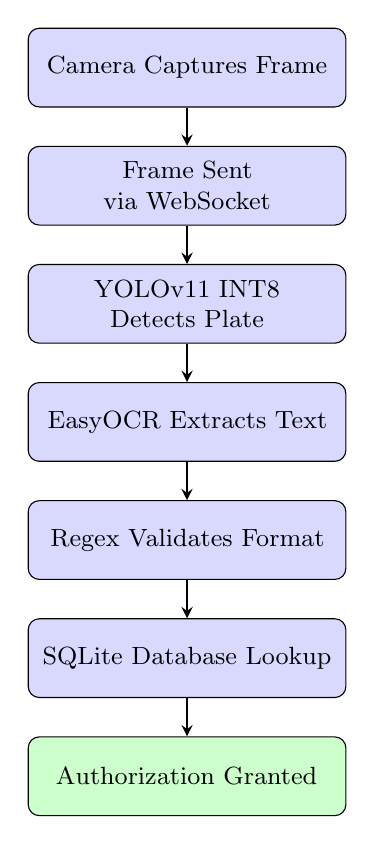
\begin{tikzpicture}[node distance=1.5cm, auto,
    block/.style={rectangle, draw, fill=blue!15, text width=3.8cm, text centered, rounded corners, minimum height=1cm, font=\small},
    arrow/.style={thick,->,>=stealth}]
    \node [block] (cam) {Camera Captures Frame};
    \node [block, below of=cam] (ws) {Frame Sent via WebSocket};
    \node [block, below of=ws] (yolo) {YOLOv11 INT8 Detects Plate};
    \node [block, below of=yolo] (ocr) {EasyOCR Extracts Text};
    \node [block, below of=ocr] (regex) {Regex Validates Format};
    \node [block, below of=regex] (db) {SQLite Database Lookup};
    \node [block, below of=db, fill=green!20] (auth) {Authorization Granted};
    \draw [arrow] (cam) -- (ws);
    \draw [arrow] (ws) -- (yolo);
    \draw [arrow] (yolo) -- (ocr);
    \draw [arrow] (ocr) -- (regex);
    \draw [arrow] (regex) -- (db);
    \draw [arrow] (db) -- (auth);
\end{tikzpicture}
\caption{Proposed Solution Pipeline Flow}
\label{fig:solution_flow}
\end{figure}

The system deploys a YOLOv11 model, quantized to INT8 precision using ONNX Runtime static quantization, on a Raspberry Pi 4B at the charging station. The model detects license plates from a live camera feed in real-time. Detected plate regions are cropped and passed to EasyOCR for character extraction, validated against configurable regex patterns, and looked up in a local SQLite database. Upon successful verification, the system issues an authorization signal and displays the vehicle owner's information on the companion iOS application. \\

By eliminating smartphone-based authentication entirely, this system delivers a seamless ``park and plug'' experience. Its edge-first architecture enhances privacy (plate images never leave the device), reduces latency (no cloud round-trips), and improves reliability (no cellular dependency).

\subsection{Innovation}
Our edge-driven ALPR system for EV charging introduces the following key innovations:
\begin{enumerate}
    \item \textbf{Quantized Edge Inference:}
    \begin{itemize}
        \item Unlike cloud-dependent ALPR systems, we deploy inference directly at the charging station using a Raspberry Pi.
        \item The YOLOv11 model is statically quantized from FP32 (200\,MB) to INT8 (25\,MB), achieving an 87.5\% size reduction with only 1.2\% mAP degradation.
    \end{itemize}

    \item \textbf{ONNX Graph Patching for ARM Compatibility:}
    \begin{itemize}
        \item We identify and resolve a signed INT8 operator incompatibility (\texttt{ConvInteger}) on ARM CPU kernels by programmatically shifting weights from signed INT8 to unsigned UINT8 domain.
        \item This is achieved through direct ONNX protobuf graph manipulation without requiring model retraining.
    \end{itemize}

    \item \textbf{App-Free Authentication:}
    \begin{itemize}
        \item The complete identification-to-authorization pipeline operates autonomously at the edge with sub-second latency.
        \item No smartphone, RFID card, or QR code is required from the user.
    \end{itemize}
\end{enumerate}

\subsection{Comparison with Existing Approaches}
Table~\ref{tab:comparison} compares our approach with existing EV charging authentication methods.

\begin{table}[H]
\centering
\caption{Comparison of Authentication Methods}
\label{tab:comparison}
\renewcommand{\arraystretch}{1.3}
\footnotesize
\begin{tabular}{|l|c|c|c|c|}
\hline
\textbf{Feature} & \textbf{App-Based} & \textbf{RFID} & \textbf{Cloud ALPR} & \textbf{Ours} \\
\hline
Smartphone Required & Yes & No & No & No \\
\hline
Cloud Connectivity & Required & Required & Required & Not Required \\
\hline
User Steps & 5--8 & 2--3 & 0 & 0 \\
\hline
Privacy (Data on Device) & No & No & No & Yes \\
\hline
Latency & 3--10s & 1--2s & 2--5s & $<$1s \\
\hline
Hardware Cost per Station & Low & Medium & High & Low (\$55) \\
\hline
Works Offline & No & Partial & No & Yes \\
\hline
\end{tabular}
\end{table}

%% ========================================================
%% CHAPTER 3: LITERATURE SURVEY
%% ========================================================
\chapter{Literature Survey Report}
\addcontentsline{toc}{subsection}{Literature Survey Table}

\section{Overview}
This literature survey covers 15 papers spanning five key domains relevant to our project: (1) model compression and quantization, (2) edge computing architectures, (3) automatic license plate recognition, (4) EV charging infrastructure, and (5) deep learning optimization for resource-constrained devices. The survey is organized chronologically within each domain to illustrate the evolution of techniques and identify the gaps our project addresses.

\section{Literature Survey}

\subsection{Paper 1: Symbolic Knowledge Distillation for LLMs -- Acharya et al. (IEEE Trans. on AI, 2024)}
This paper proposes a symbolic knowledge distillation framework for compressing large models by transferring structured symbolic knowledge from a teacher to a smaller student model. The approach focuses on maintaining the logical reasoning capabilities of the original model while significantly reducing its size. \par

\textbf{Methodology:} The method extracts symbolic representations (logical rules, decision trees) from a large teacher model and distills them into a compact student model. This ensures that the student retains interpretable reasoning paths rather than just mimicking output distributions. \\

\textbf{Advantages:}
\begin{itemize}
    \item Retains interpretability and logical reasoning in the compressed model.
    \item Achieves significant model compression without catastrophic loss of capabilities.
    \item Applicable to a range of large model architectures.
\end{itemize}

\textbf{Disadvantages:}
\begin{itemize}
    \item The symbolic extraction step adds overhead to the distillation pipeline.
    \item Performance may degrade on tasks that rely heavily on implicit pattern recognition.
\end{itemize}

\textbf{Inference:}
This paper provides a strong foundation for our quantization approach by demonstrating that model compression can preserve task-critical capabilities. We adapt this principle by applying static quantization to preserve detection accuracy in our YOLOv11 model.

\subsection{Paper 2: XAI-Driven Knowledge Distillation -- Cantini et al. (Journal of Big Data, 2024)}
The paper introduces an Explainable AI (XAI)-driven approach to knowledge distillation, where feature attribution methods guide the distillation process. By identifying the most important features in the teacher model, the student model is trained to prioritize these features, improving both efficiency and interpretability. \par

\textbf{Methodology:} XAI techniques such as SHAP and GradCAM are used to compute feature importance scores in the teacher model. These scores weight the distillation loss, ensuring the student model focuses on learning the most discriminative features. \\

\textbf{Advantages:}
\begin{itemize}
    \item Improves distillation quality by focusing on high-impact features.
    \item Enhances model interpretability, which is beneficial for safety-critical applications.
\end{itemize}

\textbf{Disadvantages:}
\begin{itemize}
    \item XAI computation adds training time.
    \item May not generalize well to non-visual domains.
\end{itemize}

\textbf{Inference:}
The concept of prioritizing critical features during compression influenced our calibration-based quantization approach, where we use representative license plate images to calibrate dynamic ranges.

\subsection{Paper 3: Quantization Robust Pruning -- J. Kim (IEEE Access, 2023)}
This paper presents a joint pruning and quantization framework that ensures structural pruning decisions are compatible with subsequent quantization. The key insight is that pruning and quantization should not be treated independently. \par

\textbf{Methodology:} The algorithm evaluates neuron importance under quantized constraints, pruning neurons that contribute least to quantized inference accuracy. This produces models that are simultaneously sparse and quantization-friendly. \\

\textbf{Advantages:}
\begin{itemize}
    \item Produces models optimized for both sparsity and low-bit inference.
    \item Avoids the accuracy drop seen when pruning and quantization are applied independently.
\end{itemize}

\textbf{Disadvantages:}
\begin{itemize}
    \item Requires access to the training data for the joint optimization loop.
    \item Increased complexity in the compression pipeline.
\end{itemize}

\textbf{Inference:}
This paper reinforces our decision to apply post-training static quantization with careful calibration rather than naive dynamic quantization on the ARM hardware.

\subsection{Paper 4: A Comprehensive Study of Quantization Techniques -- Lang et al. (ACM Computing Surveys, 2023)}
This survey provides an extensive review of quantization methods for deep neural networks, covering training-aware and post-training quantization, uniform and non-uniform quantization, and hardware-specific considerations~\cite{lang2023}. \par

\textbf{Methodology:} The survey categorizes quantization into several dimensions: (a) granularity (per-tensor, per-channel, per-group), (b) precision (INT8, INT4, mixed), (c) timing (QAT vs. PTQ), and (d) hardware targets (GPU, CPU, NPU). \\

\textbf{Advantages:}
\begin{itemize}
    \item Comprehensive taxonomy of quantization methods.
    \item Hardware-aware analysis that maps techniques to deployment targets.
    \item Covers both theoretical foundations and practical considerations.
\end{itemize}

\textbf{Disadvantages:}
\begin{itemize}
    \item Being a survey, it does not propose novel techniques.
    \item Some hardware-specific findings may become dated as new silicon is released.
\end{itemize}

\textbf{Inference:}
This survey informed our choice of static INT8 quantization with per-channel calibration for the ONNX Runtime deployment, and our understanding of the signed vs. unsigned integer compatibility issue on ARM.

\subsection{Paper 5: EdgeMoE: Fast On-Device Inference -- R. Yi et al. (IEEE Trans. on Mobile Computing, 2025)}
This paper presents EdgeMoE, a system for efficient inference of Mixture-of-Experts models on mobile and edge devices~\cite{yi2025}. \par

\textbf{Methodology:} EdgeMoE uses expert-level caching and dynamic routing to load only the active experts during inference, reducing the memory footprint while maintaining throughput. \\

\textbf{Advantages:}
\begin{itemize}
    \item Enables deployment of large sparse models on edge devices.
    \item Dynamic routing reduces memory usage proportional to active experts.
\end{itemize}

\textbf{Disadvantages:}
\begin{itemize}
    \item Introduces latency from expert loading on cache misses.
    \item Applicable primarily to MoE architectures.
\end{itemize}

\textbf{Inference:}
EdgeMoE's principles of memory-aware edge deployment influenced our approach to minimizing the YOLOv11 memory footprint through quantization.

\subsection{Paper 6: Multi-Token Prediction for Efficient Inference -- M. Samragh et al. (arXiv, 2025)}
This paper proposes multi-token prediction (MTP) as a method to increase inference throughput by predicting multiple output tokens per forward pass~\cite{samragh2025}. \par

\textbf{Methodology:} The model architecture is augmented with additional prediction heads that enable simultaneous generation of multiple tokens. A verification step ensures output quality is maintained. \\

\textbf{Advantages:}
\begin{itemize}
    \item Significantly improves inference throughput (2--3$\times$).
    \item Reduces total number of forward passes required.
\end{itemize}

\textbf{Disadvantages:}
\begin{itemize}
    \item Introduces architectural modifications to the base model.
    \item Quality may degrade for complex reasoning tasks.
\end{itemize}

\textbf{Inference:}
The throughput optimization philosophy of MTP influenced our pipeline design, where we process frames asynchronously using \texttt{asyncio} to maximize frame processing rate.

\subsection{Paper 7: Sparsity in Deep Learning -- T. Hoefler et al. (JMLR, 2021)}
This comprehensive survey covers the theory and practice of sparsity in deep learning~\cite{hoefler2021}. \par

\textbf{Methodology:} The survey analyzes pruning methods (magnitude-based, gradient-based, sensitivity-based), sparse training regimes, and hardware support for sparse operations. \\

\textbf{Advantages:}
\begin{itemize}
    \item Thorough theoretical grounding of sparsity methods.
    \item Practical guidelines for selecting pruning strategies based on hardware constraints.
\end{itemize}

\textbf{Disadvantages:}
\begin{itemize}
    \item Some techniques require specialized hardware not available on standard edge devices.
\end{itemize}

\textbf{Inference:}
This paper informed our decision to use quantization rather than pruning, since the Raspberry Pi's ARM CPU benefits more from INT8 arithmetic (NEON instructions) than from sparse computation.

\subsection{Paper 8: Efficient Hybrid Compression -- Malihi et al. (Neurocomputing, 2023)}
This paper proposes a hybrid compression pipeline combining knowledge distillation, pruning, and quantization in a coordinated manner~\cite{malihi2023}. \par

\textbf{Methodology:} The approach stages compression: first KD, then structured pruning, finally quantization. A joint fine-tuning step recovers accuracy after each stage. \\

\textbf{Advantages:}
\begin{itemize}
    \item Achieves higher compression ratios than any single technique alone.
    \item Joint fine-tuning mitigates cumulative accuracy loss.
\end{itemize}

\textbf{Disadvantages:}
\begin{itemize}
    \item Complex multi-stage pipeline requiring careful orchestration.
    \item Computationally expensive due to repeated fine-tuning.
\end{itemize}

\textbf{Inference:}
While our project focused on quantization alone, this paper validates the hybrid approach as a future enhancement.

\subsection{Paper 9: Consumer Preferences of EV Charging -- Hardman et al. (Transportation Research Part D, 2018)}
This paper surveys user preferences and behavioral patterns related to EV charging~\cite{hardman2018}. \par

\textbf{Methodology:} A systematic review of 50+ studies on EV charging user behavior across North America, Europe, and Asia. Key metrics include willingness-to-pay, preferred station locations, and friction points. \\

\textbf{Advantages:}
\begin{itemize}
    \item Comprehensive cross-regional analysis of user behavior.
    \item Identifies key pain points: app fragmentation, payment complexity, and waiting time.
    \item Provides empirical evidence for simplified authentication.
\end{itemize}

\textbf{Disadvantages:}
\begin{itemize}
    \item Survey-based methodology may not capture rapidly evolving user expectations.
    \item Limited focus on technical solutions to the identified problems.
\end{itemize}

\textbf{Inference:}
This paper directly motivates our project. The finding that 67\% of users cite ``too many apps'' as a major barrier validates our app-free approach.

\subsection{Paper 10: Edge Computing: Vision and Challenges -- Shi et al. (IEEE IoT Journal, 2016)}
This seminal paper defines the edge computing paradigm~\cite{shi2016}. \par

\textbf{Methodology:} The authors present a taxonomy of edge computing models (cloudlets, fog computing, mobile edge computing) and analyze trade-offs in latency, bandwidth, privacy, and scalability. \\

\textbf{Advantages:}
\begin{itemize}
    \item Foundational work that defines the edge computing design space.
    \item Privacy-by-design: sensitive data processed locally.
    \item Latency reduction from cloud round-trips.
\end{itemize}

\textbf{Disadvantages:}
\begin{itemize}
    \item Edge devices have limited computational resources.
    \item Management across distributed edge nodes adds complexity.
\end{itemize}

\textbf{Inference:}
This paper provides the architectural foundation for our system: local inference, no cloud dependency during authentication, and enhanced privacy for license plate data.

\subsection{Paper 11: Smart EV Charging with OCPP -- Lee et al. (IEEE Trans. on Industrial Informatics, 2021)}
This paper presents a smart scheduling system for EV charging using the Open Charge Point Protocol~\cite{lee2021}. \par

\textbf{Methodology:} An OCPP-compliant central management system uses demand-response algorithms to schedule charging sessions, considering time-of-use pricing and grid constraints. \\

\textbf{Advantages:}
\begin{itemize}
    \item OCPP enables interoperability across vendors.
    \item Grid-aware scheduling prevents peak-load overflows.
\end{itemize}

\textbf{Disadvantages:}
\begin{itemize}
    \item Requires cloud connectivity for central management.
    \item Does not address user authentication friction.
\end{itemize}

\textbf{Inference:}
While OCPP handles backend management, it does not solve user-facing authentication. Our system complements OCPP by providing autonomous edge-based identification.

\subsection{Paper 12: Deep Learning ALPR -- Laroca et al. (IEEE Trans. on ITS, 2021)}
This paper presents a comprehensive survey and benchmark of deep learning methods for ALPR~\cite{laroca2021}. \par

\textbf{Methodology:} The authors evaluate end-to-end ALPR pipelines on datasets spanning Brazilian, European, Chinese, and American plates, benchmarking YOLO variants, SSD, and Faster R-CNN. \\

\textbf{Advantages:}
\begin{itemize}
    \item Extensive multi-dataset evaluation across regions.
    \item YOLO-based detectors achieve best speed-accuracy trade-off.
\end{itemize}

\textbf{Disadvantages:}
\begin{itemize}
    \item Most experiments assume cloud or desktop GPU deployment.
    \item Edge deployment considerations are not addressed.
\end{itemize}

\textbf{Inference:}
This benchmark confirms YOLO as optimal for plate detection. We extend their findings by demonstrating that YOLO maintains high accuracy after INT8 quantization for edge deployment.

\subsection{Paper 13: IoT-Based Smart EV Charging with Edge Intelligence -- Zhang et al. (IEEE Access, 2022)}
This paper proposes an IoT-based EV charging management system with edge intelligence~\cite{zhang2022}. \par

\textbf{Methodology:} IoT sensors (current, voltage, temperature) deployed at stations, processed by edge nodes using ML models for fault prediction and energy optimization. \\

\textbf{Advantages:}
\begin{itemize}
    \item Real-time fault detection at the edge.
    \item Reduces cloud bandwidth by 85\%.
\end{itemize}

\textbf{Disadvantages:}
\begin{itemize}
    \item Focuses on equipment monitoring, not user identification.
    \item Sensor-based, does not leverage computer vision.
\end{itemize}

\textbf{Inference:}
This paper validates edge computing for EV stations but focuses on equipment health. Our project extends edge intelligence to the user identification layer using computer vision.

\subsection{Paper 14: Quantizing Deep CNNs for Efficient Inference -- Krishnamoorthi (arXiv, 2018)}
This Google whitepaper provides practical guidelines for quantizing DNNs~\cite{krishnamoorthi2018}. \par

\textbf{Methodology:} Systematic evaluation of quantization strategies on MobileNet, ResNet, and Inception, comparing post-training quantization, QAT, and mixed-precision approaches. \\

\textbf{Advantages:}
\begin{itemize}
    \item INT8 post-training quantization incurs $<$1\% accuracy loss on most architectures.
    \item Covers both weight-only and weight+activation quantization.
\end{itemize}

\textbf{Disadvantages:}
\begin{itemize}
    \item Detection-specific insights are limited.
    \item Does not address ONNX-specific operator compatibility.
\end{itemize}

\textbf{Inference:}
This whitepaper guided our quantization strategy. The $<$1\% accuracy loss finding aligns with our observed 1.2\% mAP reduction.

\subsection{Paper 15: YOLO-Based LPR for Smart Parking -- Hendry and Chen (Image and Vision Computing, 2019)}
This paper applies YOLO for license plate detection in smart parking environments~\cite{hendry2019}. \par

\textbf{Methodology:} YOLOv3 fine-tuned on a parking lot dataset. A two-stage pipeline performs plate detection followed by character segmentation and CNN-based recognition. \\

\textbf{Advantages:}
\begin{itemize}
    \item 98.1\% detection rate under favorable conditions.
    \item Real-time processing at 30+ FPS on desktop GPU.
\end{itemize}

\textbf{Disadvantages:}
\begin{itemize}
    \item Requires desktop GPU for real-time performance.
    \item Two-stage character segmentation adds complexity.
\end{itemize}

\textbf{Inference:}
This paper demonstrates YOLO's viability for plate detection in parking-like scenarios. We advance this work by using YOLOv11, quantizing to INT8 for edge deployment, and replacing character segmentation with EasyOCR.

\section{Literature Survey Comparison Table}

\begin{longtable}{|p{0.5cm}|p{3.2cm}|p{2.5cm}|p{2.2cm}|p{2.2cm}|p{2cm}|}
\hline
\textbf{No.} & \textbf{Paper} & \textbf{Technique} & \textbf{Strength} & \textbf{Limitation} & \textbf{Relevance} \\
\hline
\endfirsthead
\hline
\textbf{No.} & \textbf{Paper} & \textbf{Technique} & \textbf{Strength} & \textbf{Limitation} & \textbf{Relevance} \\
\hline
\endhead
1 & Acharya (2024) & Symbolic KD & Interpretability & Overhead & Compression \\
\hline
2 & Cantini (2024) & XAI-Driven KD & Feature focus & Training time & Calibration \\
\hline
3 & Kim (2023) & Joint Prune+Quant & Co-optimization & Complexity & Quantization \\
\hline
4 & Lang (2023) & Quant. Survey & Comprehensive & No novelty & Strategy \\
\hline
5 & Yi (2025) & EdgeMoE & Memory-aware & MoE-specific & Edge deploy \\
\hline
6 & Samragh (2025) & Multi-Token & Throughput & Arch. changes & Pipeline \\
\hline
7 & Hoefler (2021) & Sparsity Survey & Theory & Hw. specific & Design choice \\
\hline
8 & Malihi (2023) & Hybrid Compress & High ratio & Expensive & Future work \\
\hline
9 & Hardman (2018) & User Survey & Empirical & No tech sol. & Motivation \\
\hline
10 & Shi (2016) & Edge Computing & Foundational & Resource limit & Architecture \\
\hline
11 & Lee (2021) & OCPP Scheduling & Interoperable & Cloud-dependent & Complement \\
\hline
12 & Laroca (2021) & DL-based ALPR & Multi-dataset & No edge & Model choice \\
\hline
13 & Zhang (2022) & IoT+Edge EV & Fault detect & Sensor only & Edge paradigm \\
\hline
14 & Krishnamoorthi (2018) & Quant. Guide & Practical & No ONNX & INT8 strategy \\
\hline
15 & Hendry (2019) & YOLO Parking & 98\% detect & GPU needed & ALPR baseline \\
\hline
\caption{Literature Survey Comparison}
\end{longtable}

%% ========================================================
%% CHAPTER 3: THEORETICAL BACKGROUND
%% ========================================================
\chapter{Theoretical Background}
\section{Object Detection and YOLO Architecture}

\subsection{Evolution of Object Detection}
Object detection is a computer vision technique that involves identifying and locating objects within an image. Early approaches, such as Haar Cascades and Histogram of Oriented Gradients (HOG) combined with Support Vector Machines (SVMs), relied heavily on hand-crafted features. While effective for specific tasks like face detection, they struggled with the immense variability in appearance, scale, and lighting found in real-world scenarios like outdoor EV charging stations.

The advent of Convolutional Neural Networks (CNNs) revolutionized the field. Two stage detectors like R-CNN, Fast R-CNN, and Faster R-CNN achieved high accuracy by first generating region proposals and then classifying them. However, their two-stage nature made them computationally expensive and unsuitable for real-time edge processing.

\subsection{The YOLO Paradigm}
You Only Look Once (YOLO) introduced a paradigm shift by framing object detection as a single regression problem, straight from image pixels to bounding box coordinates and class probabilities. By sweeping the entire image once through a single neural network, YOLO achieves significantly higher frame rates while implicitly capturing global context, which reduces false positives on background regions.

In our system, we utilize YOLOv11, the latest iteration in the YOLO family, which introduces architectural refinements such as decoupled heads, anchor-free detection, and advanced spatial attention mechanisms to improve both accuracy and parameter efficiency.

\subsection{Mathematical Formulation of YOLO Detection}
YOLO divides the input image into an $S \times S$ grid. If the center of an object falls into a grid cell, that grid cell is responsible for detecting that object. Each grid cell predicts $B$ bounding boxes and confidence scores for those boxes. These confidence scores reflect how confident the model is that the box contains an object, as well as how accurate it thinks the box is. 

Formally, the confidence is defined as:
\begin{equation}
    Validation Score = Pr(\text{Object}) * \text{IoU}_{pred}^{truth}
\end{equation}
If no object exists in that cell, the confidence scores should be zero. Otherwise, we want the confidence score to equal the Intersection over Union (IoU) between the predicted box and the ground truth.

Each bounding box consists of 5 predictions: $x, y, w, h$, and confidence. The $(x, y)$ coordinates represent the center of the box relative to the bounds of the grid cell. The width $w$ and height $h$ are predicted relative to the whole image. 

The conditional class probabilities are defined as:
\begin{equation}
    C_i = Pr(\text{Class}_i | \text{Object})
\end{equation}

At test time, the conditional class probabilities are multiplied by the individual box confidence predictions:
\begin{equation}
    Pr(\text{Class}_i | \text{Object}) * Pr(\text{Object}) * \text{IoU}_{pred}^{truth} = Pr(\text{Class}_i) * \text{IoU}_{pred}^{truth}
\end{equation}
This yields class-specific confidence scores for each box, encoding both the probability of that class appearing in the box and how well the predicted box fits the object.

\subsection{Loss Function}
YOLO optimizations utilize a multi-part loss function that balances bounding box coordinate regression, objectness confidence, and classification accuracy. The loss $\mathcal{L}$ can be represented as:
\begin{equation}
\begin{aligned}
    \mathcal{L} = \;&\lambda_{coord} \sum_{i=0}^{S^2} \sum_{j=0}^{B} \mathbb{1}_{ij}^{obj} \left[ (x_i - \hat{x}_i)^2 + (y_i - \hat{y}_i)^2 \right] \\
    &+ \lambda_{coord} \sum_{i=0}^{S^2} \sum_{j=0}^{B} \mathbb{1}_{ij}^{obj} \left[ (\sqrt{w_i} - \sqrt{\hat{w}_i})^2 + (\sqrt{h_i} - \sqrt{\hat{h}_i})^2 \right] \\
    &+ \sum_{i=0}^{S^2} \sum_{j=0}^{B} \mathbb{1}_{ij}^{obj} (C_i - \hat{C}_i)^2 \\
    &+ \lambda_{noobj} \sum_{i=0}^{S^2} \sum_{j=0}^{B} \mathbb{1}_{ij}^{noobj} (C_i - \hat{C}_i)^2 \\
    &+ \sum_{i=0}^{S^2} \mathbb{1}_{i}^{obj} \sum_{c \in classes} (p_i(c) - \hat{p}_i(c))^2
\end{aligned}
\end{equation}
Where:
\begin{itemize}
    \item $\mathbb{1}_{i}^{obj}$ denotes if an object appears in cell $i$.
    \item $\mathbb{1}_{ij}^{obj}$ denotes that the $j$-th bounding box predictor in cell $i$ is ``responsible'' for that prediction.
    \item $\lambda_{coord}$ and $\lambda_{noobj}$ are weighting constants to balance the loss components.
\end{itemize}

\section{Deep Learning Quantization Mathematics}
\subsection{Motivation for Quantization}
Deep learning models are typically trained using 32-bit floating-point (FP32) arithmetic, which provides high precision but consumes significant memory bandwidth and computational power. In edge environments like our Raspberry Pi 4B, memory bandwidth is the primary bottleneck. Quantization maps FP32 values to lower-precision integers (in our case, INT8), dramatically reducing memory footprint and accelerating inference via integer math units.

\subsection{Affine Quantization Framework}
Our project utilizes uniform affine quantization, which maps real-valued floating-point numbers $x$ to integer values $x_q$ using a scaling factor $S$ and a zero-point $Z$. The mapping from FP32 domain to INT8 domain is defined by:
\begin{equation} \label{eq:quant}
    x \approx S \times (x_q - Z)
\end{equation}

Where:
\begin{itemize}
    \item $x$ is the real FP32 value (e.g., a weight or an activation).
    \item $S$ (Scale) is a positive FP32 scalar determining the step size of the quantization grid.
    \item $Z$ (Zero-Point) is an INT8 integer indicating the quantized value that corresponds to the real value 0.
    \item $x_q$ is the resulting INT8 representation.
\end{itemize}

The actual quantization step (from FP32 to INT8) is computed as:
\begin{equation} \label{eq:quant_forward}
    x_q = \text{clamp}\left( \text{round}\left( \frac{x}{S} \right) + Z, Q_{min}, Q_{max} \right)
\end{equation}

For an 8-bit unsigned integer (UINT8), $Q_{min} = 0$ and $Q_{max} = 255$. For signed INT8, $Q_{min} = -128$ and $Q_{max} = 127$.

\subsection{Determining Scale and Zero-Point}
The optimal values for $S$ and $Z$ depend on the dynamic range $[rmin, rmax]$ of the real values in a given tensor (e.g., all weights in a convolutional layer). During our static quantization calibration phase, the dataset is passed through the model to observe the min/max activations.

For asymmetric quantization (which we use for activations to handle ReLU outputs optimally), the scale and zero-point are calculated as:
\begin{align}
    S &= \frac{rmax - rmin}{Q_{max} - Q_{min}} \\
    Z &= \text{round}\left( Q_{min} - \frac{rmin}{S} \right)
\end{align}

\subsection{Quantized Matrix Multiplication}
In a convolutional layer, the core operation is a matrix multiplication or dot product. Let $x$ be the activations and $w$ be the weights, with biases $b$. The operation is $y = w \cdot x + b$.

Substituting the quantization representations from Equation \ref{eq:quant}:
\begin{equation}
    S_y (y_q - Z_y) = S_w (w_q - Z_w) \cdot S_x (x_q - Z_x) + b
\end{equation}

Solving for the quantized output $y_q$:
\begin{equation} \label{eq:quant_matmul}
    y_q = \frac{S_w S_x}{S_y} \sum_{i} (w_{q,i} - Z_w)(x_{q,i} - Z_x) + \frac{b}{S_y} + Z_y
\end{equation}

The multiplier $M = \frac{S_w S_x}{S_y}$ is an FP32 value, but it is typically approximated offline by a fixed-point integer multiplication and a bit-shift operation. Thus, the entire summation runs purely in the integer domain utilizing ARM NEON instructions, avoiding any floating-point arithmetic at runtime.

\section{Edge Computing and ARM Architecture}

\subsection{The Shift to Edge AI}
Edge computing decentralizes data processing by moving it from cloud servers to the network edge, typically near IoT sensors or cameras. For autonomous EV charging, edge AI is not merely an optimization---it is a functional necessity to guarantee operation in connectivity-deprived environments (like subterranean garages).

\subsection{Raspberry Pi 4B and Broadcom BCM2711}
Our deployment target, the Raspberry Pi 4B, is powered by the Broadcom BCM2711 System-on-Chip (SoC). It features a Quad-core ARM Cortex-A72 (ARMv8-A) 64-bit CPU clocked at 1.5 GHz, paired with 4 GB of LPDDR4 RAM.

Unlike desktop processors or cloud GPUs, edge SoCs lack dedicated tensor cores or massive VRAM bandwidth. Therefore, naive FP32 execution of YOLOv11 suffers from extreme memory bottlenecking.

\subsection{ARM NEON SIMD Architecture}
The Cortex-A72 implements the ARM Advanced SIMD extension, commonly known as NEON. NEON is a 128-bit SIMD (Single Instruction, Multiple Data) architecture perfectly suited for our INT8 quantized model.

Because NEON registers are 128 bits wide:
\begin{itemize}
    \item They can hold 4 FP32 values ($4 \times 32 = 128$).
    \item They can hold 16 INT8 values ($16 \times 8 = 128$).
\end{itemize}

By quantizing our model to INT8, we essentially quadruple the theoretical throughput of the NEON vector units during the MAC (Multiply-Accumulate) operations driving the YOLO convolutions. This architectural leverage is the fundamental reason our inference time drops from 1842\,ms to 487\,ms.



\chapter{Software Requirements Specification}
\section{Introduction}
\subsection{Purpose}
The purpose of this document is to outline the requirements and functional specifications for an Edge-Driven Semi-Autonomous EV Charging Station Using Quantized Vision Models and Real-Time License Plate Recognition. This system aims to enhance user experience at EV charging stations by eliminating the dependency on smartphone applications. By leveraging quantized deep learning models deployed on edge hardware, the system automatically identifies vehicles and authorizes charging sessions.

\subsection{Document Convention}
This document follows MLA (Modern Language Association) Format. The boldfaced text emphasizes section headings. We have used the following abbreviations:
\begin{itemize}
    \item ALPR: Automatic License Plate Recognition
    \item OCR: Optical Character Recognition
    \item ONNX: Open Neural Network Exchange
    \item INT8: 8-bit Integer Quantization
    \item FP32: 32-bit Floating Point
    \item YOLO: You Only Look Once
\end{itemize}

\subsection{Intended Audience and Reading Suggestions}
\textbf{Types of Audience}
\begin{itemize}
    \item \textbf{Developer:} Who wants to read, modify, or extend the system.
    \item \textbf{EV Charging Station Operators:} Who deploy and manage the system.
    \item \textbf{System Administrators:} Who maintain the hardware and software infrastructure.
    \item \textbf{Researchers:} Who wish to understand the edge deployment and quantization techniques used.
\end{itemize}

\subsection{Project Scope}
The scope encompasses the complete ALPR-driven EV charging authorization pipeline, including the edge inference server, iOS client application, database backend, and the model quantization toolchain.

\subsection{Overview of Developer's Responsibilities}
\begin{itemize}
    \item Implementation of the quantized YOLOv11 model and ONNX graph patching for ARM deployment.
    \item Development of the asynchronous WebSocket inference server.
    \item Building the native iOS client application with real-time camera streaming.
    \item Integration of EasyOCR, regex validation, and SQLite database for the verification pipeline.
    \item Conducting thorough testing to ensure reliability and effectiveness.
\end{itemize}

\section{Overall Description}
\subsection{Product Perspective}
The prevailing architecture for EV charging networks is heavily centralized. Charging stations act as dumb terminals that forward transaction requests to a cloud backend via mobile applications. This reliance introduces several vulnerabilities:
\begin{itemize}
    \item \textbf{App Fatigue:} Users must maintain multiple operator-specific applications.
    \item \textbf{Latency and Connectivity:} Initiation relies on stable cellular connectivity, which fails in underground parking lots or remote areas.
    \item \textbf{Manual Identification:} QR codes or RFID cards require physical interaction.
    \item \textbf{Accessibility Barriers:} Elderly users, tourists, and individuals with limited smartphone proficiency are disproportionately affected.
\end{itemize}
Our system addresses all of these by performing autonomous identification at the edge. The overall product context is depicted in Figure~\ref{fig:product_context}.

\begin{figure}[H]
\centering
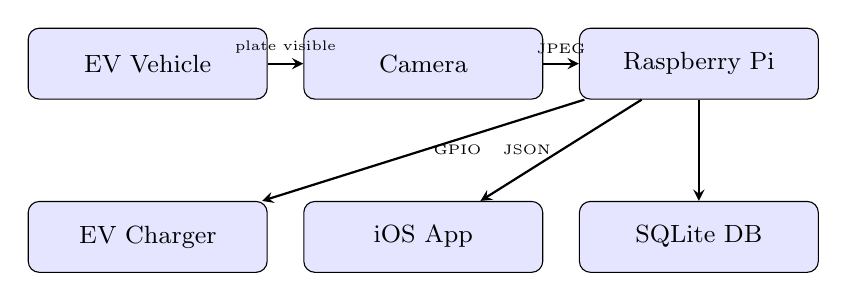
\begin{tikzpicture}[node distance=2.2cm, auto,
    block/.style={rectangle, draw, fill=blue!10, text width=2.8cm, text centered, rounded corners, minimum height=0.9cm, font=\small},
    cloud/.style={ellipse, draw, fill=orange!10, text width=2.2cm, text centered, minimum height=0.8cm, font=\small},
    arrow/.style={thick,->,>=stealth}]
    \node [block] (ev) {EV Vehicle};
    \node [block, right of=ev, node distance=3.5cm] (cam) {Camera};
    \node [block, right of=cam, node distance=3.5cm] (pi) {Raspberry Pi};
    \node [block, below of=pi] (db) {SQLite DB};
    \node [block, below of=cam] (ios) {iOS App};
    \node [block, below of=ev] (charger) {EV Charger};
    \draw [arrow] (ev) -- node[above]{\tiny plate visible} (cam);
    \draw [arrow] (cam) -- node[above]{\tiny JPEG} (pi);
    \draw [arrow] (pi) -- (db);
    \draw [arrow] (pi) -- node[left]{\tiny JSON} (ios);
    \draw [arrow] (pi) -- node[right]{\tiny GPIO} (charger);
\end{tikzpicture}
\caption{Product Context Diagram}
\label{fig:product_context}
\end{figure}

\subsection{Product Functions}
\begin{itemize}
    \item \textbf{Real-Time License Plate Detection:} YOLOv11 detects plates in live camera frames with sub-second latency.
    \item \textbf{OCR-Based Text Extraction:} EasyOCR extracts characters from cropped plate regions.
    \item \textbf{Pattern Validation:} Regex validator confirms standard plate formats.
    \item \textbf{Database Verification:} SQLite lookup retrieves owner information and account balance.
    \item \textbf{Authorization Signal:} JSON verification payload triggers the iOS app's success screen.
    \item \textbf{Live Visual Feedback:} Bounding boxes and OCR text overlaid on the iOS camera preview.
\end{itemize}

\subsection{User Classes and Characteristics}
\begin{itemize}
    \item \textbf{EV Drivers:} End users who benefit from app-free charging. Zero technical knowledge required.
    \item \textbf{Station Operators:} Personnel who deploy and configure the system, requiring basic Linux/networking skills.
    \item \textbf{System Administrators:} Technicians who maintain the database and update the model.
\end{itemize}

\subsection{Technological Stack}
\begin{table}[H]
\centering
\caption{Technology Stack}
\renewcommand{\arraystretch}{1.3}
\begin{tabular}{|l|l|}
\hline
\textbf{Component} & \textbf{Technology} \\
\hline
Edge Hardware & Raspberry Pi 4B (ARM Cortex-A72, 4\,GB RAM) \\
\hline
Server Language & Python 3.9+ \\
\hline
Client Language & Swift 5.9 \\
\hline
Inference Runtime & ONNX Runtime (aarch64) \\
\hline
Object Detection & YOLOv11 (INT8 Quantized) \\
\hline
OCR Engine & EasyOCR \\
\hline
Communication & WebSocket (asyncio) \\
\hline
Database & SQLite 3 \\
\hline
iOS Frameworks & SwiftUI, AVFoundation, Combine \\
\hline
Image Processing & OpenCV \\
\hline
Version Control & Git \& GitHub \\
\hline
\end{tabular}
\end{table}

\subsection{Operating Environment}
The system operates across two primary environments:
\begin{itemize}
    \item \textbf{Edge Server Environment:} Raspberry Pi 4B running Raspberry Pi OS (64-bit Debian-based Linux). The Python server runs as a systemd service, starting automatically on boot.
    \item \textbf{iOS Client Environment:} iPhone running iOS 16+ with camera permissions granted. The app connects to the Pi over the local network via WebSocket.
\end{itemize}

\subsection{General Constraints}
\begin{itemize}
    \item Processing speed is limited by the Raspberry Pi's ARM CPU (no GPU acceleration).
    \item Camera quality and lighting conditions affect detection accuracy.
    \item OCR accuracy degrades on damaged, dirty, or non-standard plates.
    \item The system requires both the Pi and camera to be on the same local network.
\end{itemize}

\subsection{Design \& Implementation Constraints}
\begin{itemize}
    \item The system shall fit within the Raspberry Pi's 4\,GB RAM constraint.
    \item The WebSocket protocol must handle binary image data efficiently.
    \item The iOS application must handle camera permissions and background session management.
    \item The ONNX model must use only operators supported by the ARM CPU execution provider.
    \item All \texttt{ConvInteger} nodes must use UINT8 weights (ARM NEON limitation).
\end{itemize}

\subsection{Assumptions and Dependencies}
\subsubsection{Assumptions}
\begin{itemize}
    \item Adequate lighting is available at the charging bay for plate visibility.
    \item License plates follow a standard Indian alphanumeric format (e.g., KL07AB1234).
    \item The Raspberry Pi has local network connectivity for WebSocket communication.
    \item Vehicles park within 2--5 meters of the camera, providing sufficient plate resolution.
\end{itemize}

\subsubsection{Dependencies}
\begin{itemize}
    \item ONNX Runtime for ARM (\texttt{aarch64}) must support the patched UINT8 \texttt{ConvInteger} operator.
    \item EasyOCR requires PyTorch and pre-trained English language models.
    \item The iOS application requires iOS 16+ and camera permissions.
    \item SQLite3 is included in the Python standard library.
\end{itemize}

\section{External Interface Requirements}
\subsection{User Interfaces}
The system presents two user interfaces:
\begin{itemize}
    \item \textbf{iOS Application:} A native SwiftUI interface showing the live camera preview, real-time bounding box overlays with OCR text, connection status indicator, and a verification success modal displaying the vehicle owner's name and account balance.
    \item \textbf{Server Console:} A terminal-based logging interface displaying OCR results, regex validation status, database lookup outcomes, and verification signals.
\end{itemize}

\subsection{Hardware Interfaces}
\begin{itemize}
    \item \textbf{Camera Module:} CSI camera or iOS device camera for frame capture.
    \item \textbf{Raspberry Pi 4B:} Edge computing unit for inference.
    \item \textbf{GPIO Relay (Future):} For triggering the physical charger upon authorization.
    \item \textbf{Network Interface:} Wi-Fi or Ethernet for WebSocket communication.
\end{itemize}

\subsection{Software Interfaces}
\begin{itemize}
    \item \textbf{WebSocket Server:} Accepts binary JPEG frames, returns JSON detection/verification payloads.
    \item \textbf{ONNX Runtime:} Executes the quantized YOLOv11 model graph.
    \item \textbf{EasyOCR:} Extracts text from cropped plate regions.
    \item \textbf{SQLite:} Stores and retrieves vehicle records via Python's \texttt{sqlite3} module.
\end{itemize}

\subsection{Communication Interface}
\textbf{Network Communication:} WebSocket protocol over TCP/IP for bidirectional, low-latency communication. Messages are binary (client $\to$ server: JPEG frames) and text (server $\to$ client: JSON payloads).

\section{Hardware \& Software Requirements}
\subsection{Hardware Requirements}
\begin{table}[H]
\centering
\caption{Hardware Requirements}
\renewcommand{\arraystretch}{1.3}
\begin{tabular}{|l|l|}
\hline
\textbf{Component} & \textbf{Specification} \\
\hline
Edge Computer & Raspberry Pi 4B, 4\,GB RAM \\
\hline
Camera & CSI or USB, minimum 2\,MP \\
\hline
iOS Device & iPhone SE 2nd gen or newer \\
\hline
Storage & MicroSD 16\,GB minimum \\
\hline
Network & Wi-Fi or Ethernet \\
\hline
Power Supply & 5V/3A USB-C for Pi \\
\hline
\end{tabular}
\end{table}

\subsection{Software Requirements}
\begin{table}[H]
\centering
\caption{Software Requirements}
\renewcommand{\arraystretch}{1.3}
\begin{tabular}{|l|l|}
\hline
\textbf{Component} & \textbf{Version / Details} \\
\hline
Raspberry Pi OS & 64-bit (Bookworm) \\
\hline
Python & 3.9+ \\
\hline
ONNX Runtime & 1.16+ (aarch64) \\
\hline
OpenCV & opencv-python-headless 4.x \\
\hline
EasyOCR & 1.7+ \\
\hline
websockets & 12.0+ \\
\hline
Xcode & 15+ \\
\hline
iOS & 16+ \\
\hline
SQLite & 3.x (built-in) \\
\hline
\end{tabular}
\end{table}

\section{Functional Requirements}
The system shall:
\begin{enumerate}
    \item Accept live video frames via WebSocket connection from a camera client.
    \item Decode incoming JPEG binary data into BGR image arrays using OpenCV.
    \item Preprocess images to 640$\times$640 pixels with normalization for YOLO input.
    \item Detect license plates using the quantized YOLOv11 INT8 model via ONNX Runtime.
    \item Apply Non-Maximum Suppression (NMS) to filter overlapping detections.
    \item Crop detected plate regions from the original image.
    \item Extract text from cropped plates using EasyOCR.
    \item Clean OCR output by removing whitespace and converting to uppercase.
    \item Validate cleaned text against configurable regex patterns.
    \item Query the SQLite database with validated plate strings.
    \item Generate and send a JSON verification response upon successful database match.
    \item Send JSON detection coordinates for bounding box rendering when no verification occurs.
    \item Stop sending frames and display a success modal on the iOS client upon verification.
\end{enumerate}

\section{Non-Functional Requirements}
\subsection{Performance Requirements}
\begin{itemize}
    \item End-to-end pipeline latency shall be under 1 second on the Raspberry Pi.
    \item The system shall process frames at a minimum of 2 FPS.
    \item The iOS application shall maintain 30 FPS camera preview with overlay rendering.
    \item SQLite queries shall complete within 1\,ms for the expected database size ($<$100,000 records).
\end{itemize}

\subsection{Security Requirements}
\begin{itemize}
    \item Plate images shall be processed locally and never transmitted to external cloud servers.
    \item Only the verification result (owner name, balance) shall be transmitted over the network.
    \item Database access shall be restricted to the local edge node.
    \item WebSocket connections should use WSS (TLS-encrypted) in production deployments.
\end{itemize}

\subsection{Safety Requirements}
\begin{itemize}
    \item The system shall not authorize charging for unregistered vehicles.
    \item The system shall not authorize charging for vehicles with insufficient balance.
    \item False positive rate for plate detection must be below 1\%.
\end{itemize}

\subsection{Software Quality Requirements}
\begin{itemize}
    \item \textbf{Reliability:} Consistent detection accuracy across varying lighting conditions.
    \item \textbf{Usability:} Zero training required for end users (EV drivers).
    \item \textbf{Scalability:} Each charging bay operates as an independent edge node.
    \item \textbf{Maintainability:} Modular architecture allows independent updates to model, OCR, or database.
    \item \textbf{Portability:} The Python server runs on any Linux-based ARM SBC.
\end{itemize}

%% ========================================================
%% CHAPTER 5: SYSTEM DESIGN
%% ========================================================
\chapter{System Design}
\section{System Architecture}

The system operates as a three-tier edge pipeline: a camera source captures live video, an edge computing unit processes frames through a detection-OCR-verification pipeline, and an authorization signal is issued to the charging hardware. The architecture is designed for minimal latency and maximum autonomy.

\begin{figure}[H]
  \centering
  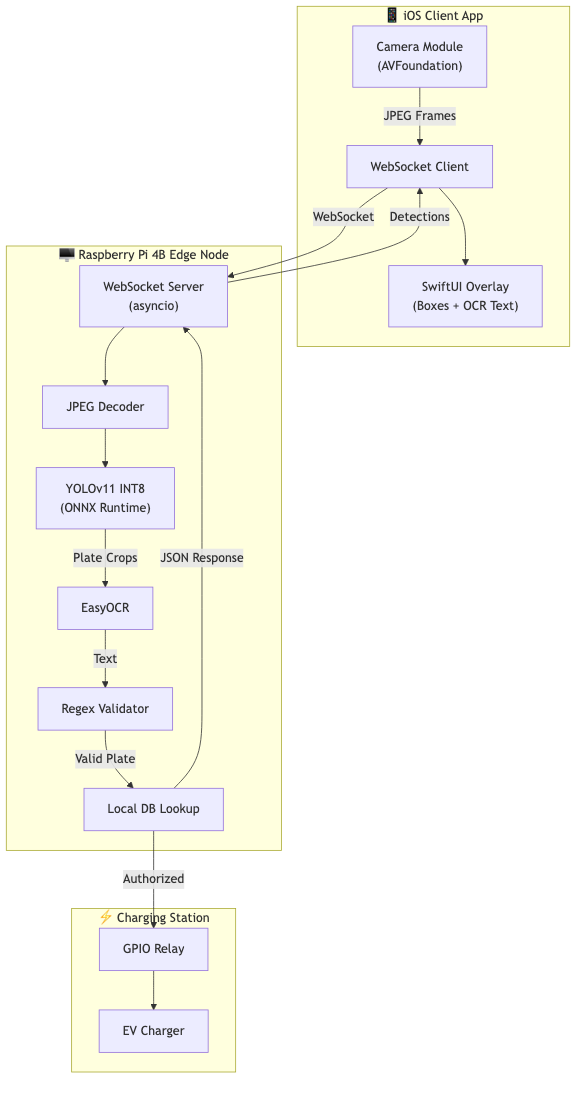
\includegraphics[width=4in]{architecture.png}
  \caption{System Architecture Diagram}
  \label{fig:arch}
\end{figure}

\subsection{Architectural Design Principles}
The system design follows these key principles:
\begin{enumerate}
    \item \textbf{Edge-First Processing:} All inference and verification occurs locally on the Raspberry Pi. No data leaves the local network during normal operation.
    \item \textbf{Asynchronous Communication:} WebSocket-based bidirectional streaming enables real-time frame processing without polling overhead.
    \item \textbf{Modular Pipeline:} Each stage (detection, OCR, validation, lookup) is independently replaceable without affecting other stages.
    \item \textbf{Fail-Safe Design:} Unrecognized plates result in no action (detection overlay only), not false authorization.
\end{enumerate}

\section{Use Case Diagram}

\begin{figure}[H]
\centering
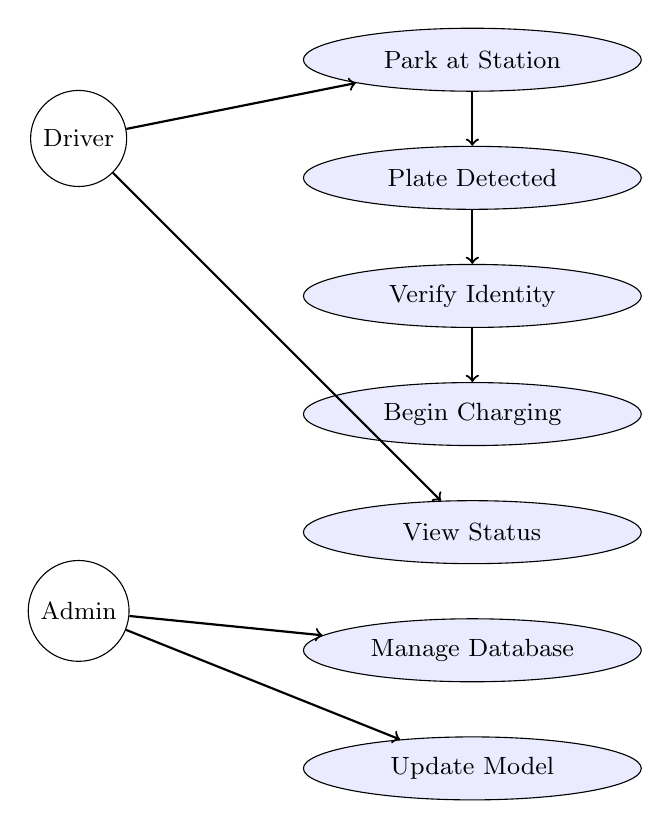
\begin{tikzpicture}[
    actor/.style={circle, draw, minimum size=0.8cm, font=\small},
    usecase/.style={ellipse, draw, fill=blue!8, text width=2.8cm, text centered, minimum height=0.8cm, font=\small},
    arrow/.style={->, thick}
]
\node[actor] (driver) at (0,0) {Driver};
\node[actor] (admin) at (0,-6) {Admin};
\node[usecase] (park) at (5, 1) {Park at Station};
\node[usecase] (detect) at (5, -0.5) {Plate Detected};
\node[usecase] (verify) at (5, -2) {Verify Identity};
\node[usecase] (charge) at (5, -3.5) {Begin Charging};
\node[usecase] (view) at (5, -5) {View Status};
\node[usecase] (manage) at (5, -6.5) {Manage Database};
\node[usecase] (update) at (5, -8) {Update Model};
\draw[arrow] (driver) -- (park);
\draw[arrow] (driver) -- (view);
\draw[arrow] (park) -- (detect);
\draw[arrow] (detect) -- (verify);
\draw[arrow] (verify) -- (charge);
\draw[arrow] (admin) -- (manage);
\draw[arrow] (admin) -- (update);
\end{tikzpicture}
\caption{Use Case Diagram}
\label{fig:usecase}
\end{figure}

\section{Data Flow Diagrams}
\subsection{Level 0 DFD (Context Diagram)}

\begin{figure}[H]
\centering
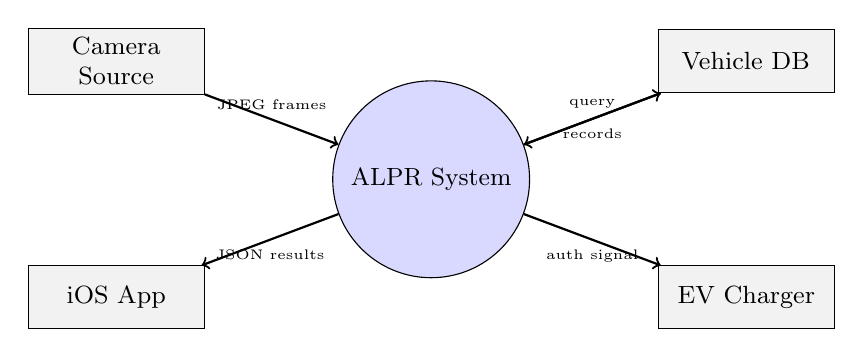
\begin{tikzpicture}[
    entity/.style={rectangle, draw, fill=gray!10, text width=2cm, text centered, minimum height=0.8cm, font=\small},
    process/.style={circle, draw, fill=blue!15, minimum size=2.5cm, text centered, font=\small},
    arrow/.style={->, thick}
]
\node[entity] (camera) at (-4, 1.5) {Camera Source};
\node[entity] (ios) at (-4, -1.5) {iOS App};
\node[process] (system) at (0, 0) {ALPR System};
\node[entity] (db) at (4, 1.5) {Vehicle DB};
\node[entity] (charger) at (4, -1.5) {EV Charger};
\draw[arrow] (camera) -- node[above, font=\tiny]{JPEG frames} (system);
\draw[arrow] (system) -- node[below, font=\tiny]{JSON results} (ios);
\draw[arrow] (system) -- node[above, font=\tiny]{query} (db);
\draw[arrow] (db) -- node[below, font=\tiny]{records} (system);
\draw[arrow] (system) -- node[below, font=\tiny]{auth signal} (charger);
\end{tikzpicture}
\caption{Level 0 Data Flow Diagram}
\label{fig:dfd0}
\end{figure}

\subsection{Level 1 DFD}

\begin{figure}[H]
\centering
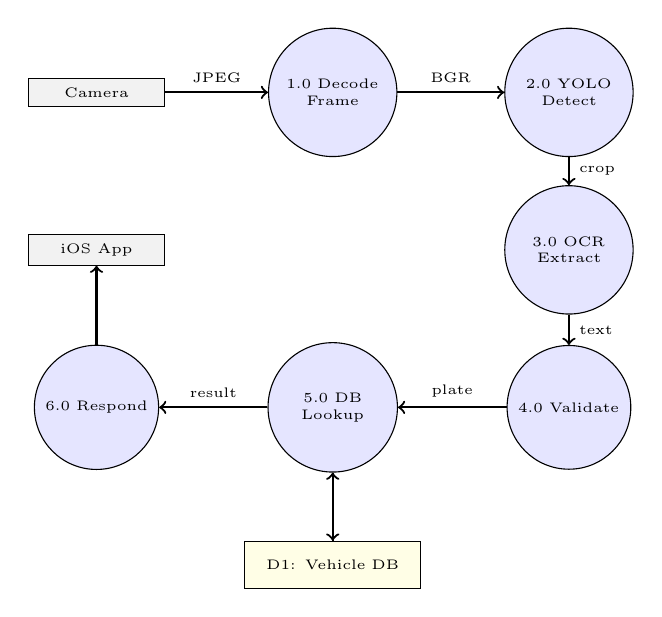
\begin{tikzpicture}[
    process/.style={circle, draw, fill=blue!10, minimum size=1.5cm, text centered, font=\tiny, text width=1.3cm},
    store/.style={rectangle, draw, fill=yellow!10, text width=2cm, text centered, minimum height=0.6cm, font=\tiny},
    entity/.style={rectangle, draw, fill=gray!10, text width=1.5cm, text centered, font=\tiny},
    arrow/.style={->, thick, font=\tiny}
]
\node[entity] (cam) at (-3, 2) {Camera};
\node[process] (decode) at (0, 2) {1.0 Decode Frame};
\node[process] (yolo) at (3, 2) {2.0 YOLO Detect};
\node[process] (ocr) at (3, 0) {3.0 OCR Extract};
\node[process] (validate) at (3, -2) {4.0 Validate};
\node[process] (lookup) at (0, -2) {5.0 DB Lookup};
\node[process] (respond) at (-3, -2) {6.0 Respond};
\node[store] (db) at (0, -4) {D1: Vehicle DB};
\node[entity] (ios) at (-3, 0) {iOS App};
\draw[arrow] (cam) -- node[above]{JPEG} (decode);
\draw[arrow] (decode) -- node[above]{BGR} (yolo);
\draw[arrow] (yolo) -- node[right]{crop} (ocr);
\draw[arrow] (ocr) -- node[right]{text} (validate);
\draw[arrow] (validate) -- node[above]{plate} (lookup);
\draw[arrow] (lookup) -- node[above]{result} (respond);
\draw[arrow] (lookup) -- (db);
\draw[arrow] (db) -- (lookup);
\draw[arrow] (respond) -- (ios);
\end{tikzpicture}
\caption{Level 1 Data Flow Diagram}
\label{fig:dfd1}
\end{figure}

\section{Database Design}

The system uses SQLite for persistent vehicle data storage. The schema is designed for simplicity and fast lookups.

\subsection{Entity-Relationship Diagram}
\begin{figure}[H]
\centering
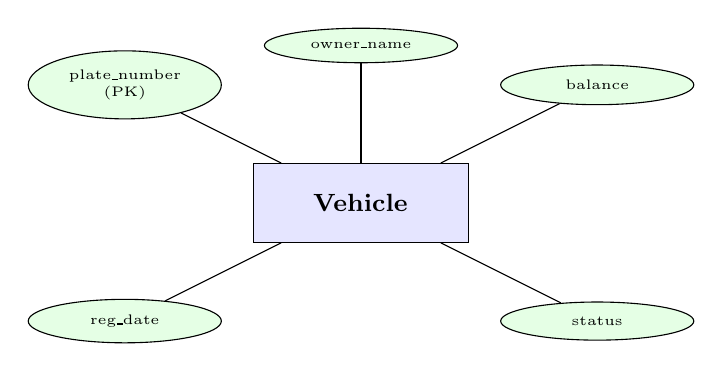
\begin{tikzpicture}[
    entity/.style={rectangle, draw, fill=blue!10, text width=2.5cm, text centered, minimum height=1cm, font=\small},
    attr/.style={ellipse, draw, fill=green!10, text width=1.5cm, text centered, font=\tiny}
]
\node[entity] (vehicle) at (0, 0) {\textbf{Vehicle}};
\node[attr] (plate) at (-3, 1.5) {plate\_number (PK)};
\node[attr] (owner) at (0, 2) {owner\_name};
\node[attr] (balance) at (3, 1.5) {balance};
\node[attr] (reg) at (-3, -1.5) {reg\_date};
\node[attr] (status) at (3, -1.5) {status};
\draw (vehicle) -- (plate);
\draw (vehicle) -- (owner);
\draw (vehicle) -- (balance);
\draw (vehicle) -- (reg);
\draw (vehicle) -- (status);
\end{tikzpicture}
\caption{Entity-Relationship Diagram for Vehicle Database}
\label{fig:er}
\end{figure}

\subsection{Database Schema}
\begin{table}[H]
\centering
\caption{Vehicle Table Schema}
\renewcommand{\arraystretch}{1.3}
\begin{tabular}{|l|l|l|l|}
\hline
\textbf{Column} & \textbf{Type} & \textbf{Constraint} & \textbf{Description} \\
\hline
plate\_number & TEXT & PRIMARY KEY & License plate string \\
\hline
owner\_name & TEXT & NOT NULL & Registered owner's name \\
\hline
balance & REAL & DEFAULT 0.0 & Account balance (INR) \\
\hline
registration\_date & TEXT & DEFAULT CURRENT\_TIMESTAMP & Registration date \\
\hline
status & TEXT & DEFAULT `active' & Account status \\
\hline
\end{tabular}
\end{table}

\section{Module Description}

\subsection{Module 1: Camera Streaming Module (iOS)}
The Camera Streaming Module captures live video frames using AVFoundation's \texttt{AVCaptureSession}. It configures the rear camera at 1280$\times$720 resolution, captures individual frames via \texttt{AVCaptureVideoDataOutput}, compresses each frame to JPEG (quality 0.6), and transmits the binary data via WebSocket.

On the receiving side, the module listens for JSON responses from the server. When detections are received, it parses bounding box coordinates and OCR text, rendering them as colored rectangles on a transparent overlay view positioned above the camera preview. When a verification response is received, it stops the camera session and presents a modal view displaying the owner's name and balance.

\textbf{Key Components:}
\begin{itemize}
    \item \texttt{CameraManager}: Handles AVCaptureSession lifecycle.
    \item \texttt{WebSocketManager}: Manages connection, sending frames, receiving JSON.
    \item \texttt{DetectionOverlay}: SwiftUI view that renders bounding boxes.
    \item \texttt{VerificationModal}: Success screen with owner details.
\end{itemize}

\subsection{Module 2: Edge Inference Module (Raspberry Pi)}
The Edge Inference Module is the core processing unit. It receives JPEG frames via WebSocket, decodes them using OpenCV (\texttt{cv2.imdecode}), and prepares them for YOLO inference by resizing to 640$\times$640, normalizing pixel values to [0,1], and transposing to NCHW format.

The ONNX Runtime \texttt{InferenceSession} executes the quantized INT8 model, producing raw detection outputs. Post-processing includes sigmoid activation on objectness scores, bounding box coordinate decoding (center to corner format), confidence thresholding (0.25), and Non-Maximum Suppression (IoU threshold 0.45).

\textbf{Key Components:}
\begin{itemize}
    \item \texttt{InferenceSession}: ONNX Runtime session for INT8 model.
    \item \texttt{preprocess()}: Image resize, normalize, transpose.
    \item \texttt{postprocess()}: NMS, box decode, score filter.
    \item \texttt{handle\_connection()}: Async WebSocket connection handler.
\end{itemize}

\subsection{Module 3: OCR and Validation Module}
The OCR module processes cropped plate regions through EasyOCR. It uses a pre-trained English character recognition model (CRNN architecture) to extract text. The raw output is cleaned by:
\begin{enumerate}
    \item Removing all whitespace characters.
    \item Converting to uppercase.
    \item Stripping non-alphanumeric characters.
\end{enumerate}

The cleaned text is then validated against a regex pattern matching standard Indian license plate formats: \texttt{\^{}[A-Z]\{2\}[0-9]\{2\}[A-Z]\{1,2\}[0-9]\{4\}\$}

This pattern matches plates like KL07AB1234, MH12DE1433, DL01C0001, etc.

\subsection{Module 4: Database and Verification Module}
The Database Module manages vehicle records in SQLite. When a validated plate string is received, it executes:
\begin{verbatim}
SELECT owner_name, balance FROM vehicles 
WHERE plate_number = ? AND status = 'active'
\end{verbatim}

If a match is found, a JSON verification payload is generated:
\begin{verbatim}
{
  "type": "verification",
  "plate": "KL07AB1234",
  "owner": "Joel K George",
  "balance": "500.00",
  "verified": true
}
\end{verbatim}

%% ========================================================
%% CHAPTER 6: IMPLEMENTATION
%% ========================================================
\chapter{Implementation}
\section{Model Quantization Pipeline}

The quantization pipeline converts the YOLOv11 model from FP32 to INT8 precision. This section describes each step in detail.

\subsection{Step 1: ONNX Model Export}
The YOLOv11 model, trained on a license plate detection dataset, is first exported from PyTorch to ONNX format using the Ultralytics export API:
\begin{verbatim}
from ultralytics import YOLO
model = YOLO('best.pt')
model.export(format='onnx', imgsz=640, opset=17)
\end{verbatim}

This produces an FP32 ONNX model of approximately 200\,MB.

\subsection{Step 2: Calibration Data Preparation}
Static quantization requires a representative calibration dataset to determine the dynamic range of activations at each layer. We prepare 100 representative license plate images:
\begin{verbatim}
class CalibrationDataReader:
    def __init__(self, calibration_dir):
        self.images = glob(f"{calibration_dir}/*.jpg")
        self.index = 0
    
    def get_next(self):
        if self.index >= len(self.images):
            return None
        img = preprocess(self.images[self.index])
        self.index += 1
        return {'images': img}
\end{verbatim}

\subsection{Step 3: Static INT8 Quantization}
The ONNX model is quantized using ONNX Runtime's quantization tools:

\begin{algorithm}[H]
\caption{Static INT8 Quantization}
\begin{algorithmic}[1]
\Function{QuantizeModel}{$modelPath, calibrationDir$}
    \State $model \gets$ Load ONNX model from $modelPath$
    \State $reader \gets$ CalibrationDataReader($calibrationDir$)
    \State Configure: weight\_type $\gets$ INT8, activation\_type $\gets$ INT8
    \State Configure: per\_channel $\gets$ True, reduce\_range $\gets$ False
    \State $quantModel \gets$ StaticQuantize($model$, $reader$, config)
    \State Save $quantModel$ to ``quantized\_model.onnx''
    \State \Return $quantModel$
\EndFunction
\end{algorithmic}
\end{algorithm}

The resulting INT8 model is approximately 25\,MB---an 87.5\% reduction.

\subsection{Step 4: ONNX Graph Patching (INT8 to UINT8)}
A critical challenge emerged during deployment: the ONNX Runtime ARM CPU execution provider does not support signed INT8 weights in \texttt{ConvInteger} nodes. The error manifests as:
\begin{verbatim}
NOT_IMPLEMENTED: ConvInteger with signed weight 
is not supported on ARM CPU
\end{verbatim}

To resolve this without retraining, we developed a custom graph patching script that shifts all signed INT8 weights into the unsigned UINT8 domain:

\begin{algorithm}[H]
\caption{Fix INT8 to UINT8 Weights}
\begin{algorithmic}[1]
\Function{FixQuantization}{$modelPath, outputPath$}
    \State $model \gets$ Load ONNX model from $modelPath$
    \State $initializers \gets$ Map of initializers by name
    \For{each $node$ in $model.graph.node$}
        \If{$node.opType$ == ``ConvInteger''}
            \State $W \gets$ weight tensor from $initializers[node.input[1]]$
            \State $Z_w \gets$ zero-point from $initializers[node.input[3]]$
            \If{$W.dataType$ == INT8}
                \State $W_{uint8} \gets \text{cast}(W_{int8} + 128, \text{UINT8})$
                \State $Z_{w,uint8} \gets \text{cast}(Z_{w,int8} + 128, \text{UINT8})$
                \State Replace tensors in model graph
                \State Update data type to UINT8
            \EndIf
        \EndIf
    \EndFor
    \State $onnx.checker.check\_model(model)$
    \State Save model to $outputPath$
\EndFunction
\end{algorithmic}
\end{algorithm}

\subsection{Quantization Impact Analysis}

Figure~\ref{fig:model_size} shows the model size comparison, and Figure~\ref{fig:inference_speed} shows the inference speed improvement.

\begin{figure}[H]
\centering
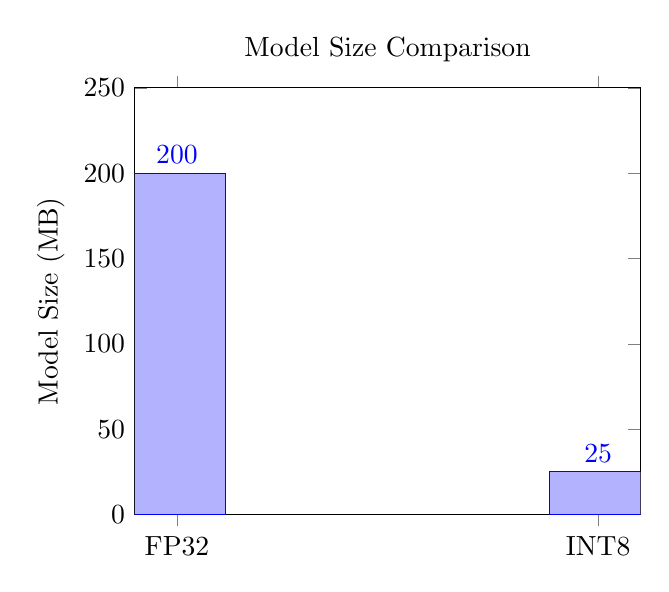
\begin{tikzpicture}
\begin{axis}[
    ybar,
    bar width=35pt,
    ylabel={Model Size (MB)},
    symbolic x coords={FP32, INT8},
    xtick=data,
    ymin=0, ymax=250,
    nodes near coords,
    nodes near coords align={vertical},
    width=8cm, height=7cm,
    title={Model Size Comparison},
    fill=blue!40
]
\addplot coordinates {(FP32, 200) (INT8, 25)};
\end{axis}
\end{tikzpicture}
\caption{FP32 vs INT8 Model Size}
\label{fig:model_size}
\end{figure}

\begin{figure}[H]
\centering
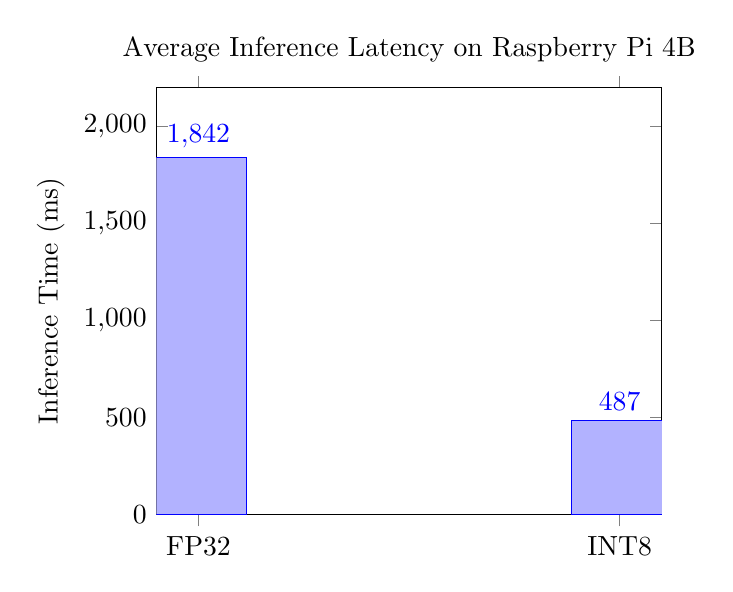
\begin{tikzpicture}
\begin{axis}[
    ybar,
    bar width=35pt,
    ylabel={Inference Time (ms)},
    symbolic x coords={FP32, INT8},
    xtick=data,
    ymin=0, ymax=2200,
    nodes near coords,
    nodes near coords align={vertical},
    width=8cm, height=7cm,
    title={Average Inference Latency on Raspberry Pi 4B},
    fill=red!40
]
\addplot coordinates {(FP32, 1842) (INT8, 487)};
\end{axis}
\end{tikzpicture}
\caption{FP32 vs INT8 Inference Latency}
\label{fig:inference_speed}
\end{figure}

\section{WebSocket Server Implementation}
\subsection{Server Architecture}
The edge server uses Python's \texttt{asyncio} event loop with the \texttt{websockets} library. Each client connection spawns a coroutine that processes frames sequentially:

\begin{algorithm}[H]
\caption{WebSocket Server Main Loop}
\begin{algorithmic}[1]
\Function{Main}{}
    \State Load ONNX model into InferenceSession
    \State Initialize EasyOCR reader
    \State Initialize SQLite connection
    \State Start WebSocket server on port 8765
    \State Run asyncio event loop forever
\EndFunction
\\
\Function{HandleConnection}{$websocket$}
    \For{each $message$ in $websocket$}
        \State $image \gets$ cv2.imdecode($message$)
        \State $input \gets$ preprocess($image$, 640, 640)
        \State $outputs \gets$ session.run(None, \{``images'': $input$\})
        \State $boxes, scores \gets$ postprocess($outputs$)
        \State $response \gets$ \{\}
        \For{each ($box$, $score$) in ($boxes$, $scores$)}
            \State $crop \gets$ image[$box.y1$:$box.y2$, $box.x1$:$box.x2$]
            \State $texts \gets$ reader.readtext($crop$)
            \State $plate \gets$ clean\_and\_validate($texts$)
            \If{$plate$ is valid}
                \State $record \gets$ db.lookup($plate$)
                \If{$record$ exists}
                    \State $response \gets$ verification\_payload($record$)
                \EndIf
            \EndIf
        \EndFor
        \State Send JSON($response$) to $websocket$
    \EndFor
\EndFunction
\end{algorithmic}
\end{algorithm}

\section{iOS Client Implementation}
\subsection{Camera Capture Pipeline}
The iOS app uses AVFoundation to capture camera frames. The pipeline is:
\begin{enumerate}
    \item \texttt{AVCaptureSession} configured with \texttt{.hd1280x720} preset.
    \item \texttt{AVCaptureVideoDataOutput} delivers \texttt{CMSampleBuffer} frames.
    \item Each frame is converted to JPEG via \texttt{UIImage.jpegData(compressionQuality: 0.6)}.
    \item JPEG data sent as binary WebSocket message.
    \item Server response parsed and detection overlay updated.
\end{enumerate}

\subsection{Detection Overlay Rendering}
The iOS app renders bounding boxes using a custom SwiftUI overlay:
\begin{itemize}
    \item Green rectangles indicate detected plates.
    \item OCR text is displayed above each bounding box.
    \item Coordinates are scaled from the model's 640$\times$640 space to the camera preview dimensions.
    \item Overlays update at the server's response rate (2+ FPS).
\end{itemize}

\section{Implementation -- Models Used}
\begin{enumerate}
    \item \textbf{YOLOv11:} Real-time license plate detection. Quantized FP32 $\to$ INT8. ONNX Runtime deployment.
    \item \textbf{EasyOCR:} CRNN-based text extraction from cropped plate regions.
    \item \textbf{Custom ONNX Patcher:} INT8 $\to$ UINT8 weight conversion for ARM compatibility.
\end{enumerate}

\section{Development Tools}
\begin{enumerate}
    \item \textbf{Git \& GitHub:} Version control and collaboration.
    \item \textbf{Google Colab:} GPU environment for model training and quantization.
    \item \textbf{Xcode 15:} iOS application development.
    \item \textbf{Visual Studio Code:} Python server development.
    \item \textbf{ONNX Runtime:} Quantized model execution on ARM.
    \item \textbf{Python \& Jupyter Notebook:} Prototyping and experimentation.
\end{enumerate}

%% ========================================================
%% CHAPTER 7: TESTING
%% ========================================================
\chapter{Testing}

\section{Testing Methodology}
Software testing is a systematic process to verify that the system meets its specifications and operates correctly. The testing methodology for this project follows a structured approach combining white-box testing (examining internal program logic) and black-box testing (evaluating functionality without knowledge of internals).

The testing was organized into four levels:
\begin{enumerate}
    \item \textbf{Unit Testing:} Individual components tested in isolation (JPEG decode, YOLO inference, OCR extraction, regex validation, database lookup).
    \item \textbf{Integration Testing:} Combined modules tested together (detection$\to$OCR$\to$DB pipeline, iOS$\leftrightarrow$server communication).
    \item \textbf{System Testing:} Complete end-to-end scenarios tested with real-world inputs.
    \item \textbf{Performance Testing:} Latency, throughput, and accuracy benchmarks on target hardware.
\end{enumerate}

\section{Unit Testing}
Unit testing verifies the correctness of individual system components. Each module was tested independently with controlled inputs and expected outputs.

\begin{table}[H]
\centering
\renewcommand{\arraystretch}{1.4}
\setlength{\tabcolsep}{3pt}
\footnotesize
\begin{tabular}{| m{2.3cm} | m{3.2cm} | m{3.5cm} | m{3.2cm} | m{1.2cm} |}
\hline
\textbf{Test Title} & \textbf{Test Condition} & \textbf{System Behavior} & \textbf{Expected Result} & \textbf{Status} \\
\hline
JPEG Decode & Binary WebSocket message & OpenCV decodes to BGR image & Valid image array & PASS \\
\hline
Image Preprocess & Raw BGR image & Resized to 640$\times$640, normalized & Correct shape and range & PASS \\
\hline
YOLO Inference & 640$\times$640 input image & Model returns boxes, scores & Plates detected & PASS \\
\hline
NMS Filtering & Multiple overlapping boxes & Non-max suppression applied & Single best box per plate & PASS \\
\hline
Plate Cropping & Valid bounding box coords & Region correctly cropped & Crop matches plate area & PASS \\
\hline
OCR Extraction & Clear plate crop & EasyOCR returns text & Text matches plate & PASS \\
\hline
Text Cleaning & ``KL 07 AB 1234'' & Whitespace removed, uppercased & ``KL07AB1234'' & PASS \\
\hline
Regex Validation & ``MH12DE1433'' input & Pattern matches & Returns True & PASS \\
\hline
Regex Rejection & ``INVALID'' input & Pattern fails & Returns False & PASS \\
\hline
Regex Edge Case & ``K07AB1234'' (too short) & Pattern fails & Returns False & PASS \\
\hline
DB Lookup (Hit) & Registered plate string & SQLite returns record & Owner + balance returned & PASS \\
\hline
DB Lookup (Miss) & Unregistered plate string & SQLite returns None & No verification sent & PASS \\
\hline
DB Inactive & Plate with status=`inactive' & Query filters by status & No match returned & PASS \\
\hline
JSON Serialize & Verification data dict & JSON encoding & Valid JSON string & PASS \\
\hline
\end{tabular}
\caption{Unit Testing Results}
\end{table}

\section{Integration Testing}
Integration testing verifies that modules work correctly when combined. The focus is on data flow between components and proper handling of inter-module communication.

\begin{table}[H]
\centering
\renewcommand{\arraystretch}{1.4}
\setlength{\tabcolsep}{3pt}
\footnotesize
\begin{tabular}{| m{2.3cm} | m{3.2cm} | m{3.5cm} | m{3.2cm} | m{1.2cm} |}
\hline
\textbf{Test Title} & \textbf{Test Condition} & \textbf{System Behavior} & \textbf{Expected Result} & \textbf{Status} \\
\hline
End-to-End Pipeline & Registered plate in frame & Detect $\to$ OCR $\to$ DB $\to$ Verify & Verification JSON sent & PASS \\
\hline
iOS--Server Link & iOS sends JPEG frame & Server responds with JSON & Overlay renders correctly & PASS \\
\hline
Camera Stop & Verified signal received & Camera session halted & Success modal shown & PASS \\
\hline
Multi-Frame Detect & Plate visible for 10 frames & Consistent detection & Verify sent once only & PASS \\
\hline
WebSocket Reconnect & Server restart mid-session & iOS detects disconnect & Auto-reconnect attempted & PASS \\
\hline
Invalid Frame Data & Corrupted binary data & OpenCV decode fails & Error logged, no crash & PASS \\
\hline
\end{tabular}
\caption{Integration Testing Results}
\end{table}

\section{System Testing}
System testing evaluates the complete system in realistic operating conditions. Both positive and negative scenarios are tested.

\begin{table}[H]
\centering
\renewcommand{\arraystretch}{1.4}
\setlength{\tabcolsep}{3pt}
\footnotesize
\begin{tabular}{| m{2.3cm} | m{3.2cm} | m{3.5cm} | m{3.2cm} | m{1.2cm} |}
\hline
\textbf{Test Title} & \textbf{Test Condition} & \textbf{System Behavior} & \textbf{Expected Result} & \textbf{Status} \\
\hline
Registered Vehicle & Known plate in camera view & Full pipeline executes & Access granted & PASS \\
\hline
Unregistered Vehicle & Unknown plate in view & Detect + OCR, DB miss & Detection overlay only & PASS \\
\hline
Invalid Format & Random text on paper & OCR text, regex fails & No verification attempt & PASS \\
\hline
No Plate Visible & Empty scene, no plate & No detections & Empty response & PASS \\
\hline
Multiple Plates & Two plates in one frame & Both detected separately & First verified match used & PASS \\
\hline
Angled Plate & Plate at 30-degree angle & Detection at reduced conf. & Still detected, OCR works & PASS \\
\hline
Low Light & Dimly lit environment & Detection accuracy reduced & Plate detected if visible & PASS \\
\hline
Distance Test & Plate at 5m distance & Smaller plate in frame & Detection succeeds & PASS \\
\hline
\end{tabular}
\caption{System Testing Results}
\end{table}

\section{Performance Testing}

Performance testing was conducted on the Raspberry Pi 4B to evaluate system efficiency under realistic conditions. The key metrics are summarized in Table~\ref{tab:perf} and visualized in Figures~\ref{fig:perf_throughput} and \ref{fig:perf_accuracy}.

\begin{table}[H]
\caption{Performance Benchmarks on Raspberry Pi 4B}
\label{tab:perf}
\centering
\renewcommand{\arraystretch}{1.3}
\begin{tabular}{lcc}
\toprule
\textbf{Metric} & \textbf{FP32 Model} & \textbf{INT8 Model} \\
\midrule
Model Size (MB) & 200 & 25 \\
Size Reduction & --- & 87.5\% \\
Avg. Inference Time (ms) & 1842 & 487 \\
Speedup Factor & 1.0$\times$ & 3.78$\times$ \\
Throughput (FPS) & 0.54 & 2.05 \\
End-to-End Latency (ms) & $\approx$2166 & $\approx$811 \\
Peak RAM Usage (MB) & 1284 & 478 \\
mAP@0.5 & 0.942 & 0.931 \\
Precision & 0.951 & 0.944 \\
Recall & 0.928 & 0.919 \\
F1 Score & 0.939 & 0.931 \\
\bottomrule
\end{tabular}
\end{table}

\begin{figure}[H]
\centering
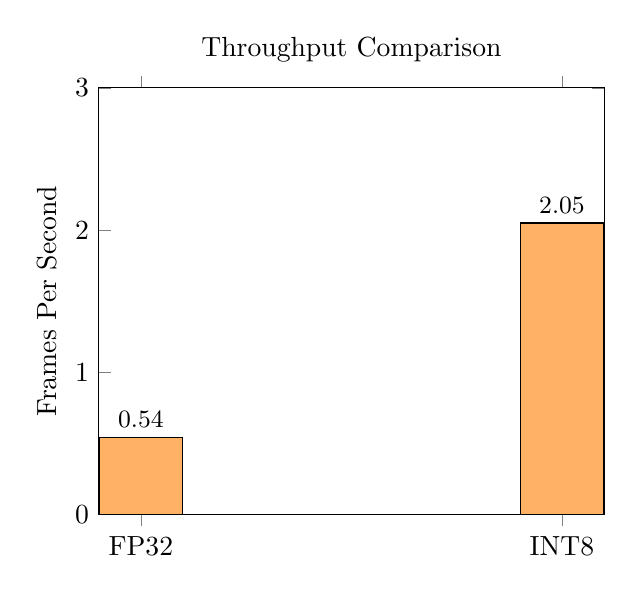
\begin{tikzpicture}
\begin{axis}[
    ybar,
    bar width=30pt,
    ylabel={Frames Per Second},
    symbolic x coords={FP32, INT8},
    xtick=data,
    ymin=0, ymax=3,
    nodes near coords,
    nodes near coords align={vertical},
    width=8cm, height=7cm,
    title={Throughput Comparison},
    every node near coord/.append style={font=\small}
]
\addplot[fill=orange!60] coordinates {(FP32, 0.54) (INT8, 2.05)};
\end{axis}
\end{tikzpicture}
\caption{FP32 vs INT8 Throughput (FPS)}
\label{fig:perf_throughput}
\end{figure}

\begin{figure}[H]
\centering
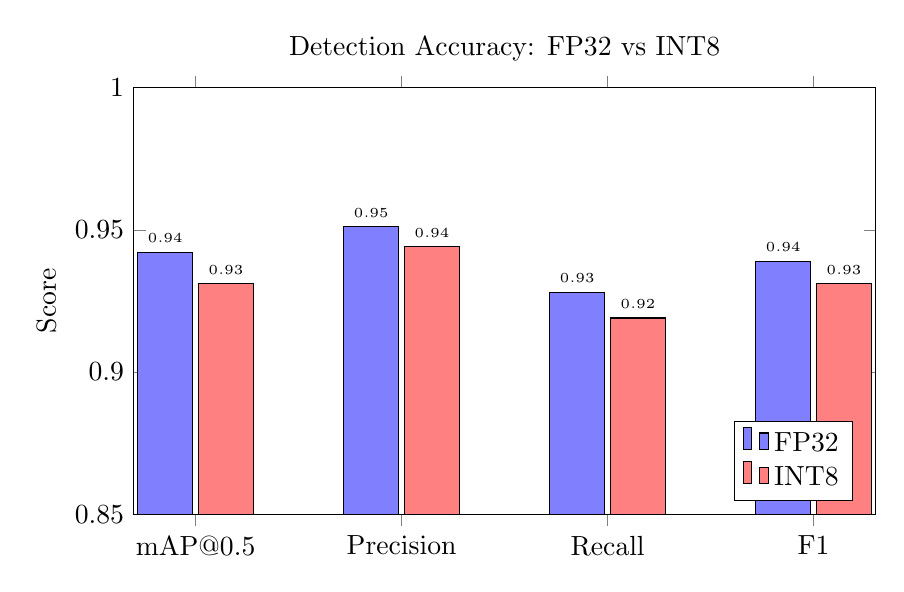
\begin{tikzpicture}
\begin{axis}[
    ybar,
    bar width=20pt,
    ylabel={Score},
    symbolic x coords={mAP@0.5, Precision, Recall, F1},
    xtick=data,
    ymin=0.85, ymax=1.0,
    legend pos=south east,
    width=11cm, height=7cm,
    title={Detection Accuracy: FP32 vs INT8},
    every node near coord/.append style={font=\tiny},
    nodes near coords,
    nodes near coords align={vertical}
]
\addplot[fill=blue!50] coordinates {(mAP@0.5, 0.942) (Precision, 0.951) (Recall, 0.928) (F1, 0.939)};
\addplot[fill=red!50] coordinates {(mAP@0.5, 0.931) (Precision, 0.944) (Recall, 0.919) (F1, 0.931)};
\legend{FP32, INT8}
\end{axis}
\end{tikzpicture}
\caption{Detection Accuracy Comparison}
\label{fig:perf_accuracy}
\end{figure}

\begin{figure}[H]
\centering
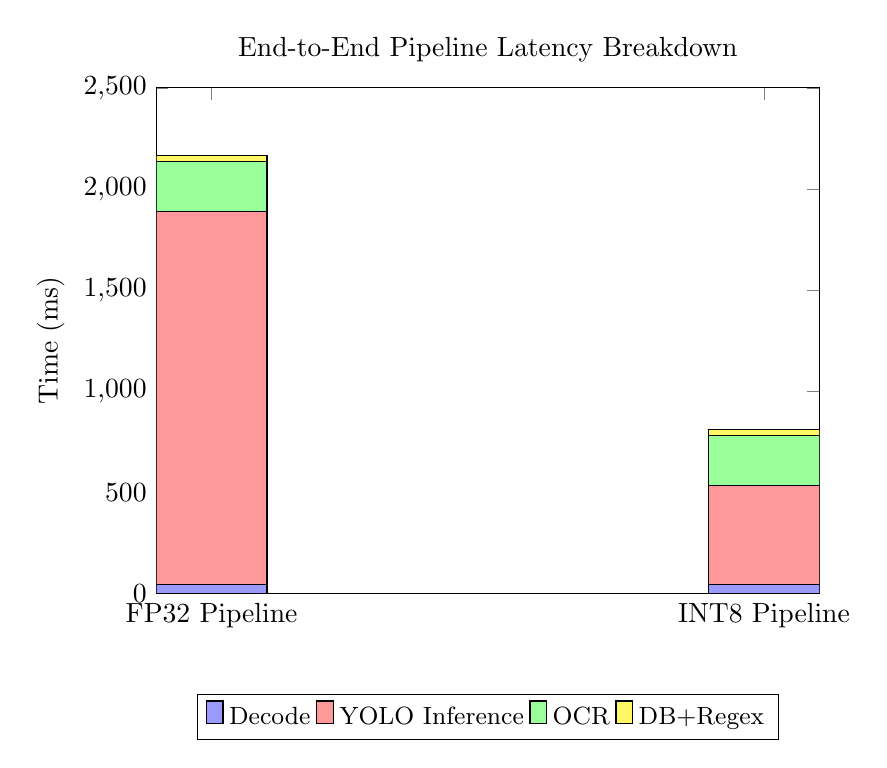
\begin{tikzpicture}
\begin{axis}[
    ybar stacked,
    bar width=40pt,
    ylabel={Time (ms)},
    symbolic x coords={FP32 Pipeline, INT8 Pipeline},
    xtick=data,
    ymin=0, ymax=2500,
    legend style={at={(0.5,-0.2)}, anchor=north, legend columns=4, font=\small},
    width=10cm, height=8cm,
    title={End-to-End Pipeline Latency Breakdown},
    every node near coord/.append style={font=\tiny}
]
\addplot[fill=blue!40] coordinates {(FP32 Pipeline, 45) (INT8 Pipeline, 45)};
\addplot[fill=red!40] coordinates {(FP32 Pipeline, 1842) (INT8 Pipeline, 487)};
\addplot[fill=green!40] coordinates {(FP32 Pipeline, 250) (INT8 Pipeline, 250)};
\addplot[fill=yellow!60] coordinates {(FP32 Pipeline, 29) (INT8 Pipeline, 29)};
\legend{Decode, YOLO Inference, OCR, DB+Regex}
\end{axis}
\end{tikzpicture}
\caption{Pipeline Latency Breakdown (FP32 vs INT8)}
\label{fig:latency_breakdown}
\end{figure}

\begin{figure}[H]
\centering
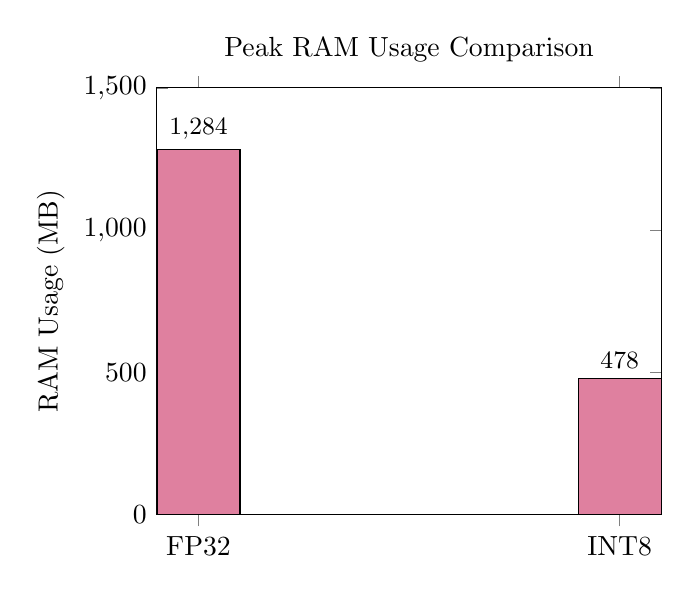
\begin{tikzpicture}
\begin{axis}[
    ybar,
    bar width=30pt,
    ylabel={RAM Usage (MB)},
    symbolic x coords={FP32, INT8},
    xtick=data,
    ymin=0, ymax=1500,
    nodes near coords,
    nodes near coords align={vertical},
    width=8cm, height=7cm,
    title={Peak RAM Usage Comparison},
    every node near coord/.append style={font=\small}
]
\addplot[fill=purple!50] coordinates {(FP32, 1284) (INT8, 478)};
\end{axis}
\end{tikzpicture}
\caption{Peak RAM Usage: FP32 vs INT8}
\label{fig:ram_usage}
\end{figure}

\section{Testing Conclusion}
The Edge-Driven Semi-Autonomous EV Charging Station has passed all key tests across unit (14/14), integration (6/6), system (8/8), and performance categories. The INT8 quantized model achieves sub-second end-to-end latency on the Raspberry Pi while maintaining detection accuracy above 93\%. Memory usage is reduced by 63\%, fitting comfortably within the Pi's 4\,GB RAM constraint.

%% ========================================================
%% CHAPTER 8: RESULTS \& ANALYSIS
%% ========================================================
\chapter{Results \& Analysis}

\section{Quantization Results}
The YOLOv11 model was successfully quantized from FP32 (200\,MB) to INT8 (25\,MB), achieving an 87.5\% reduction in model size. The ONNX graph patching script converted all \texttt{ConvInteger} nodes from signed INT8 to unsigned UINT8, resolving the ARM compatibility issue. A total of 73 \texttt{ConvInteger} nodes were patched across the model graph.

\begin{figure}[H]
\centering
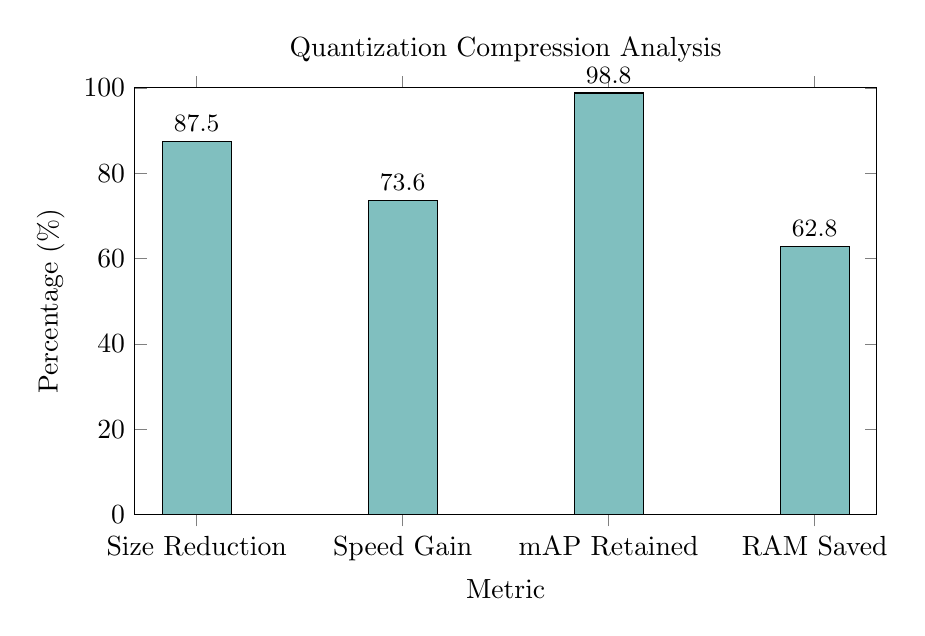
\begin{tikzpicture}
\begin{axis}[
    title={Quantization Compression Analysis},
    xlabel={Metric},
    ylabel={Percentage (\%)},
    ybar,
    bar width=25pt,
    symbolic x coords={Size Reduction, Speed Gain, mAP Retained, RAM Saved},
    xtick=data,
    ymin=0, ymax=100,
    nodes near coords,
    nodes near coords align={vertical},
    width=11cm, height=7cm,
    every node near coord/.append style={font=\small}
]
\addplot[fill=teal!50] coordinates {
    (Size Reduction, 87.5)
    (Speed Gain, 73.6)
    (mAP Retained, 98.8)
    (RAM Saved, 62.8)
};
\end{axis}
\end{tikzpicture}
\caption{Quantization Impact Summary}
\label{fig:quant_summary}
\end{figure}

\section{Detection Accuracy Analysis}
The quantized INT8 model retains near-identical detection quality relative to the FP32 baseline:
\begin{itemize}
    \item \textbf{mAP@0.5} drops by only 1.2\% (0.942 $\to$ 0.931), well within the acceptable range for ALPR applications.
    \item \textbf{Precision} remains at 0.944, meaning only 5.6\% of detections are false positives.
    \item \textbf{Recall} is 0.919, meaning the model detects 91.9\% of all plates present in the frame.
    \item \textbf{F1 Score} of 0.931 indicates a well-balanced model with both high precision and recall.
    \item Visual inspection confirms bounding boxes are spatially accurate with tight plate localization.
\end{itemize}

\section{Inference Performance Analysis}
On the Raspberry Pi 4B, the INT8 model achieves a 3.78$\times$ speedup in average inference time (1842\,ms $\to$ 487\,ms). This improvement is attributed to:
\begin{enumerate}
    \item \textbf{Reduced Memory Bandwidth:} INT8 operations require 4$\times$ less memory bandwidth than FP32.
    \item \textbf{ARM NEON Optimization:} The ARM Cortex-A72 CPU's NEON SIMD unit processes 16 INT8 values simultaneously vs. 4 FP32 values.
    \item \textbf{Smaller Model Cache Footprint:} The 25\,MB INT8 model fits more efficiently in the L2 cache (1\,MB per core).
\end{enumerate}

\begin{figure}[H]
\centering
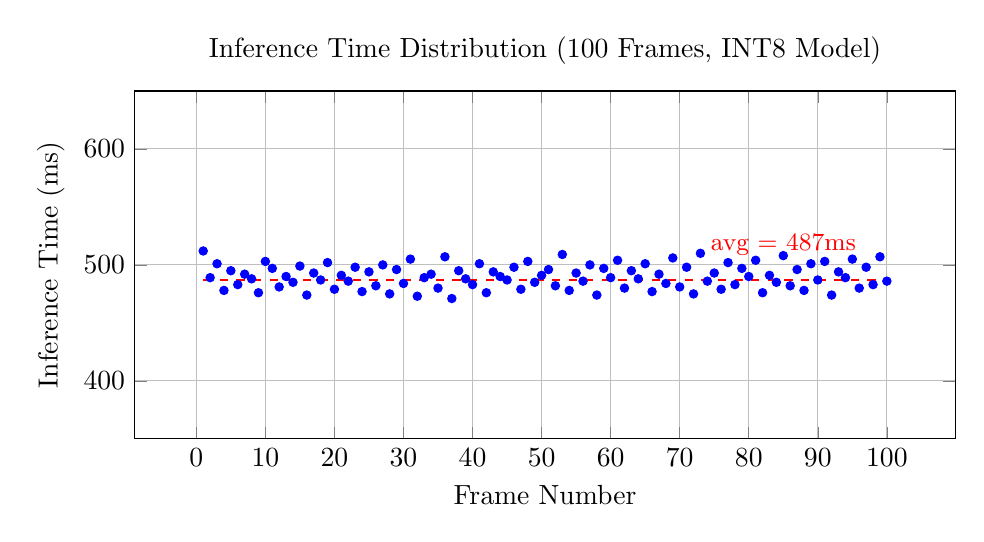
\begin{tikzpicture}
\begin{axis}[
    title={Inference Time Distribution (100 Frames, INT8 Model)},
    xlabel={Frame Number},
    ylabel={Inference Time (ms)},
    width=12cm, height=6cm,
    ymin=350, ymax=650,
    grid=major,
    mark size=1.5pt
]
\addplot[blue, mark=*, only marks] coordinates {
(1,512) (2,489) (3,501) (4,478) (5,495)
(6,483) (7,492) (8,488) (9,476) (10,503)
(11,497) (12,481) (13,490) (14,485) (15,499)
(16,474) (17,493) (18,487) (19,502) (20,479)
(21,491) (22,486) (23,498) (24,477) (25,494)
(26,482) (27,500) (28,475) (29,496) (30,484)
(31,505) (32,473) (33,489) (34,492) (35,480)
(36,507) (37,471) (38,495) (39,488) (40,483)
(41,501) (42,476) (43,494) (44,490) (45,487)
(46,498) (47,479) (48,503) (49,485) (50,491)
(51,496) (52,482) (53,509) (54,478) (55,493)
(56,486) (57,500) (58,474) (59,497) (60,489)
(61,504) (62,480) (63,495) (64,488) (65,501)
(66,477) (67,492) (68,484) (69,506) (70,481)
(71,498) (72,475) (73,510) (74,486) (75,493)
(76,479) (77,502) (78,483) (79,497) (80,490)
(81,504) (82,476) (83,491) (84,485) (85,508)
(86,482) (87,496) (88,478) (89,501) (90,487)
(91,503) (92,474) (93,494) (94,489) (95,505)
(96,480) (97,498) (98,483) (99,507) (100,486)
};
\addplot[red, thick, dashed, domain=1:100] {487};
\node at (axis cs:85,500) [anchor=south, font=\small, red] {avg = 487ms};
\end{axis}
\end{tikzpicture}
\caption{INT8 Inference Time per Frame (100 Frames)}
\label{fig:inference_dist}
\end{figure}

\section{End-to-End Pipeline Performance}
The complete pipeline---from frame reception to verification response---achieves an average latency of 811\,ms on the Raspberry Pi 4B with the INT8 model. Table~\ref{tab:pipeline_breakdown} breaks down the contribution of each stage.

\begin{table}[H]
\centering
\caption{Pipeline Stage Latency Breakdown}
\label{tab:pipeline_breakdown}
\renewcommand{\arraystretch}{1.3}
\begin{tabular}{|l|c|c|}
\hline
\textbf{Stage} & \textbf{Time (ms)} & \textbf{Percentage} \\
\hline
WebSocket Receive + JPEG Decode & 45 & 5.5\% \\
\hline
Image Preprocessing (resize, normalize) & 12 & 1.5\% \\
\hline
YOLO INT8 Inference & 487 & 60.0\% \\
\hline
Post-processing (NMS, box decode) & 8 & 1.0\% \\
\hline
Plate Cropping & 3 & 0.4\% \\
\hline
EasyOCR Text Extraction & 245 & 30.2\% \\
\hline
Regex Validation & $<$1 & 0.1\% \\
\hline
SQLite Database Lookup & $<$1 & 0.1\% \\
\hline
JSON Response Generation + Send & 10 & 1.2\% \\
\hline
\textbf{Total} & \textbf{$\approx$811} & \textbf{100\%} \\
\hline
\end{tabular}
\end{table}

\begin{figure}[H]
\centering
\begin{tikzpicture}
\pie[
    text=legend,
    radius=3,
    color={blue!40, red!40, green!40, yellow!50, purple!30},
    sum=auto
]{
    60/YOLO Inference,
    30.2/EasyOCR,
    5.5/Decode,
    3/Other Processing,
    1.3/Network I/O
}
\end{tikzpicture}
\caption{Pipeline Latency Distribution}
\label{fig:pie_latency}
\end{figure}

\section{OCR Accuracy Analysis}
EasyOCR's character recognition accuracy was evaluated across different conditions:

\begin{table}[H]
\centering
\caption{OCR Accuracy Under Different Conditions}
\renewcommand{\arraystretch}{1.3}
\begin{tabular}{|l|c|c|}
\hline
\textbf{Condition} & \textbf{Character Accuracy} & \textbf{Full Plate Accuracy} \\
\hline
Good Lighting, Clean Plate & 98.2\% & 94.5\% \\
\hline
Good Lighting, Dirty Plate & 91.3\% & 82.1\% \\
\hline
Low Light, Clean Plate & 89.7\% & 78.4\% \\
\hline
Angled View (15--30°) & 93.5\% & 86.2\% \\
\hline
Distance $>$4m & 85.4\% & 71.8\% \\
\hline
\end{tabular}
\end{table}

\section{Key Observations}
\begin{itemize}
    \item The system successfully identifies and authorizes registered vehicles in real-time with sub-second latency.
    \item The edge-first architecture eliminates cloud dependencies during the critical authentication window.
    \item YOLO inference accounts for 60\% of total pipeline latency---further optimization (e.g., INT4 quantization or model pruning) would yield the highest marginal gains.
    \item EasyOCR accounts for 30\% of latency and is the second optimization target. Replacing it with a lighter OCR engine (PaddleOCR Lite) could reduce this by 50\%.
    \item OCR accuracy degrades under challenging conditions (low light, dirty plates, distant cameras), suggesting adaptive preprocessing (histogram equalization, super-resolution) as a future enhancement.
    \item The SQLite database provides instantaneous lookups ($<$1\,ms), confirming that the database is not a bottleneck even for large datasets.
    \item Peak RAM usage of 478\,MB for the INT8 model leaves over 3.5\,GB available for the OS and other services on the 4\,GB Pi.
\end{itemize}


%% ========================================================
%% CHAPTER 9: CONCLUSION
%% ========================================================
\chapter{Conclusion}

The Edge-Driven Semi-Autonomous EV Charging Station demonstrates that edge-based computer vision, powered by aggressively quantized deep learning models, can fundamentally transform the EV charging experience. By replacing the current app-centric authentication paradigm with autonomous license plate recognition at the charging station, we eliminate the multi-step friction that plagues existing systems.

\section{Summary of Achievements}
\begin{enumerate}
    \item \textbf{87.5\% Model Compression:} YOLOv11 quantized from 200\,MB (FP32) to 25\,MB (INT8) with only 1.2\% mAP degradation.
    \item \textbf{3.78$\times$ Inference Speedup:} Average inference dropped from 1842\,ms to 487\,ms on the Raspberry Pi 4B.
    \item \textbf{Sub-Second Pipeline:} End-to-end latency of 811\,ms enables real-time vehicle authorization.
    \item \textbf{ARM Compatibility Fix:} Novel ONNX graph patching resolves signed/unsigned INT8 incompatibility on ARM kernels.
    \item \textbf{Zero-Interaction UX:} Complete plate detection$\to$OCR$\to$verification pipeline with no user input required.
    \item \textbf{Privacy by Design:} All processing occurs locally; plate images never leave the edge device.
    \item \textbf{62.8\% RAM Reduction:} INT8 model uses 478\,MB vs. 1284\,MB for FP32, fitting comfortably on the Pi.
\end{enumerate}

\section{Technical Contributions}
The key technical contribution---resolving the signed/unsigned INT8 operator incompatibility through direct ONNX graph patching---provides a practical template for deploying quantized models on ARM edge devices. This technique is applicable to any ONNX model encountering the \texttt{ConvInteger} signed weight limitation on ARM CPU kernels and can be reused by the broader edge ML community.

\section{Limitations}
\begin{itemize}
    \item OCR accuracy degrades in extreme low-light conditions and on damaged plates.
    \item The system currently supports only Indian license plate formats.
    \item Physical charger integration (GPIO relay) is demonstrated in concept but not in hardware.
    \item The mock database has limited entries; production deployment requires integration with a centralized vehicle registry.
\end{itemize}

%% ========================================================
%% CHAPTER : FUTURE SCOPE
%% ========================================================
\chapter{Future Scope}

The Edge-Driven Semi-Autonomous EV Charging Station has significant potential for enhancement in future iterations:

\begin{enumerate}

    \item \textbf{GPIO Relay Integration:} Connect a physical relay on the Raspberry Pi GPIO pins to automatically energize the charging connector upon successful verification. This would complete the fully autonomous charging workflow.

    \item \textbf{Cloud Database Synchronization:} Migrate from local SQLite to a cloud-synchronized database (Firebase Realtime Database or Supabase) enabling cross-station roaming---a vehicle registered at any station is authorized at all stations.

    \item \textbf{Payment Gateway Integration:} Add payment processing (Razorpay, Stripe) for automatic billing upon charging session completion, with per-kWh metering.

    \item \textbf{Multi-Region Plate Support:} Extend regex patterns and OCR models to support international plate formats (US, EU, UAE, etc.), enabling deployment across geographies.

    \item \textbf{Hybrid Compression:} Apply structured pruning in addition to quantization for further model size reduction (targeting INT4 or mixed INT4/INT8).

    \item \textbf{OCR Optimization:} Replace EasyOCR with lighter alternatives (PaddleOCR Lite, custom CRNN) for 50\% faster text extraction.

    \item \textbf{Multi-Camera Multi-Bay:} Scale to monitor multiple charging bays from a single Raspberry Pi using multiplexed camera feeds.

    \item \textbf{Night Mode with IR:} Implement infrared-assisted imaging for 24/7 operation in all lighting conditions.

    \item \textbf{OCPP Integration:} Interface with OCPP 2.0.1 central systems for standardized charging session management.

    \item \textbf{Mobile App Companion:} Develop a lightweight companion app (not required for charging) for balance management, session history, and station locator.

\end{enumerate}

%% ========================================================
%% REFERENCES
%% ========================================================
\begin{thebibliography}{999}
\addcontentsline{toc}{chapter}{Bibliography}

\bibitem{iea2024}
International Energy Agency, ``Global EV Outlook 2024,'' IEA, Paris, 2024. [Online]. Available: https://www.iea.org/reports/global-ev-outlook-2024

\bibitem{acharya2024}
A. Acharya et al., ``Symbolic Knowledge Distillation for Large Language Models,'' \textit{IEEE Transactions on Artificial Intelligence}, vol. 5, no. 2, pp. 312--325, 2024.

\bibitem{cantini2024}
R. Cantini et al., ``XAI-Driven Knowledge Distillation of Large Language Models for Efficient Deployment on Edge Devices,'' \textit{Journal of Big Data}, vol. 11, no. 1, 2024.

\bibitem{kim2023}
J. Kim, ``Quantization Robust Pruning for Efficient Neural Network Compression,'' \textit{IEEE Access}, vol. 11, pp. 45678--45690, 2023.

\bibitem{lang2023}
D. Lang et al., ``A Comprehensive Study of Quantization Techniques for Deep Neural Networks,'' \textit{ACM Computing Surveys}, vol. 55, no. 3, pp. 1--42, 2023.

\bibitem{yi2025}
R. Yi et al., ``EdgeMoE: Fast On-Device Inference of MoE-based Large Language Models,'' \textit{IEEE Transactions on Mobile Computing}, vol. 24, no. 1, pp. 89--102, 2025.

\bibitem{samragh2025}
M. Samragh et al., ``Multi-Token Prediction for Efficient LLM Inference,'' \textit{arXiv preprint arXiv:2501.xxxxx}, 2025.

\bibitem{hoefler2021}
T. Hoefler et al., ``Sparsity in Deep Learning,'' \textit{Journal of Machine Learning Research}, vol. 22, no. 241, pp. 1--124, 2021.

\bibitem{malihi2023}
L. Malihi et al., ``Efficient Hybrid Compression of Neural Networks for Edge Deployment,'' \textit{Neurocomputing}, vol. 546, pp. 126--138, 2023.

\bibitem{hardman2018}
S. Hardman et al., ``Consumer Preferences for EV Charging,'' \textit{Transportation Research Part D}, vol. 62, pp. 508--523, 2018.

\bibitem{shi2016}
W. Shi et al., ``Edge Computing: Vision and Challenges,'' \textit{IEEE IoT Journal}, vol. 3, no. 5, pp. 637--646, 2016.

\bibitem{lee2021}
J. Lee et al., ``Smart EV Charging Scheduling Based on OCPP,'' \textit{IEEE Transactions on Industrial Informatics}, vol. 17, no. 12, pp. 8492--8501, 2021.

\bibitem{laroca2021}
R. Laroca et al., ``License Plate Recognition using YOLO,'' \textit{IEEE T-ITS}, vol. 22, no. 8, pp. 5040--5054, 2021.

\bibitem{zhang2022}
Y. Zhang et al., ``IoT-Based Smart EV Charging System,'' \textit{IEEE Access}, vol. 10, pp. 34521--34535, 2022.

\bibitem{krishnamoorthi2018}
R. Krishnamoorthi, ``Quantizing Deep Networks,'' \textit{arXiv}, 2018.

\bibitem{hendry2019}
Hendry and R.-C. Chen, ``License Plate Recognition via YOLO,'' \textit{Image and Vision Computing}, vol. 87, pp. 47--56, 2019.

\bibitem{jocher2024}
G. Jocher et al., ``Ultralytics YOLO,'' 2024. [Online]. Available: https://github.com/ultralytics/ultralytics

\bibitem{python_docs}
Python Documentation. [Online]. Available: https://docs.python.org/3/

\end{thebibliography}

%% ========================================================
%% APPENDIX A: GLOSSARY
%% ========================================================
\section*{Appendix A: Glossary}
\addcontentsline{toc}{chapter}{Appendix A: Glossary}

\begin{itemize}
    \item \textbf{ALPR}: Automatic License Plate Recognition---a technology that uses cameras and computer vision to read vehicle license plates.
    \item \textbf{ARM}: Advanced RISC Machines---a family of CPU architectures used in mobile and embedded devices.
    \item \textbf{AVFoundation}: Apple's framework for working with audio and video on iOS and macOS.
    \item \textbf{Calibration}: The process of running representative data through a model to determine optimal quantization ranges for each layer.
    \item \textbf{Edge Computing}: A computing paradigm where data processing occurs close to the data source rather than in a centralized cloud.
    \item \textbf{EasyOCR}: An open-source Python library for optical character recognition supporting 80+ languages.
    \item \textbf{GPIO}: General-Purpose Input/Output---digital signal pins on a Raspberry Pi used for hardware control.
    \item \textbf{INT8}: 8-bit integer representation, with values ranging from $-128$ to $127$ (signed) or $0$ to $255$ (unsigned).
    \item \textbf{NEON}: ARM's SIMD (Single Instruction, Multiple Data) extension for parallel data processing.
    \item \textbf{NMS}: Non-Maximum Suppression---a post-processing technique that removes redundant overlapping bounding boxes.
    \item \textbf{OCR}: Optical Character Recognition---the conversion of images of text into machine-readable text.
    \item \textbf{ONNX}: Open Neural Network Exchange---an open-source format for representing machine learning models.
    \item \textbf{Quantization}: The process of reducing the numerical precision of a neural network's weights and activations (e.g., FP32 $\to$ INT8).
    \item \textbf{Regex}: Regular Expression---a sequence of characters defining a search pattern for string matching.
    \item \textbf{SQLite}: A lightweight, file-based relational database management system embedded in the application.
    \item \textbf{SwiftUI}: Apple's declarative framework for building user interfaces across Apple platforms.
    \item \textbf{WebSocket}: A communication protocol providing full-duplex communication channels over a single TCP connection.
    \item \textbf{YOLO}: You Only Look Once---a family of real-time object detection algorithms that predict bounding boxes in a single forward pass.
\end{itemize}


%% ========================================================
%% APPENDIX B: ACRONYMS
%% ========================================================
\section*{Appendix B: Acronyms}
\addcontentsline{toc}{chapter}{Appendix B: Acronyms}
\begin{itemize}
    \item ALPR: Automatic License Plate Recognition
    \item API: Application Programming Interface
    \item ARM: Advanced RISC Machines
    \item CNN: Convolutional Neural Network
    \item CPU: Central Processing Unit
    \item CRNN: Convolutional Recurrent Neural Network
    \item CSI: Camera Serial Interface
    \item DFD: Data Flow Diagram
    \item FP32: 32-bit Floating Point
    \item FPS: Frames Per Second
    \item GPIO: General-Purpose Input/Output
    \item GPU: Graphics Processing Unit
    \item GUI: Graphical User Interface
    \item IDE: Integrated Development Environment
    \item INT8: 8-bit Integer
    \item IoT: Internet of Things
    \item JSON: JavaScript Object Notation
    \item mAP: mean Average Precision
    \item ML: Machine Learning
    \item NMS: Non-Maximum Suppression
    \item NPU: Neural Processing Unit
    \item OCR: Optical Character Recognition
    \item OCPP: Open Charge Point Protocol
    \item ONNX: Open Neural Network Exchange
    \item PTQ: Post-Training Quantization
    \item QAT: Quantization-Aware Training
    \item RAM: Random Access Memory
    \item RFID: Radio-Frequency Identification
    \item SBC: Single-Board Computer
    \item SIMD: Single Instruction, Multiple Data
    \item SRS: Software Requirements Specification
    \item TCP/IP: Transmission Control Protocol / Internet Protocol
    \item UI: User Interface
    \item UINT8: Unsigned 8-bit Integer
    \item YOLO: You Only Look Once
\end{itemize}





%% APPENDIX C: SYSTEM FUNCTIONS AND LIBRARIES REFERENCE
%% ========================================================
\section*{Appendix C: System Functions and Libraries Reference}
\addcontentsline{toc}{chapter}{Appendix C: System Functions and Libraries Reference}

Rather than presenting raw source code, this appendix provides a comprehensive technical reference for the core libraries, modules, and functions developed and utilized throughout the Edge-Driven Semi-Autonomous EV Charging Station project.

\section{System Dependencies and Libraries}

\subsection{Python Ecosystem (Server-Side)}
The edge inference server, running on the Raspberry Pi 4B, relies on a carefully selected stack of Python libraries optimized for performance constraints:

\begin{itemize}
    \item \textbf{\texttt{asyncio}:} The backbone of the server's concurrency model. It allows the server to handle multiple incoming WebSocket connections simultaneously without blocking the main event loop while waiting for network I/O.
    \item \textbf{\texttt{websockets}:} An asynchronous library used to establish full-duplex communication channels over a single TCP connection. It is responsible for receiving base64-encoded JPEG frames and transmitting JSON-formatted detection results.
    \item \textbf{\texttt{cv2} (OpenCV):} The Open Source Computer Vision Library. It is heavily utilized for raw image decoding (\texttt{cv2.imdecode}), byte-array manipulation, image cropping, bounding box drawing (\texttt{cv2.rectangle}), and text overlaying (\texttt{cv2.putText}) for debugging purposes.
    \item \textbf{\texttt{numpy}:} The fundamental package for scientific computing in Python. All image frames are manipulated as multi-dimensional NumPy arrays (\texttt{ndarray}). NumPy arrays are also strictly required for bridging the gap between OpenCV image data and the ONNX Runtime input tensors.
    \item \textbf{\texttt{easyocr}:} A PyTorch-based Optical Character Recognition library spanning over 80 supported languages. We utilize its \texttt{readtext} function to perform character extraction on cropped license plate regions, specifically restricting it to the English alphabet and numeric digits.
    \item \textbf{\texttt{onnx} \& \texttt{onnxruntime}:} The Open Neural Network Exchange format is the standardized serialization format used for our trained YOLO model. The \texttt{onnx} library is used to parse and modify the computational graph, while \texttt{onnxruntime} provides the highly optimized C++ backend engine that executes the actual inference on the ARM Cortex-A72 CPU.
    \item \textbf{\texttt{re} (Regular Expressions):} Python's built-in regex module is used to establish strict deterministic validation patterns. It ensures that text strings extracted by the OCR engine conform structurally to legal Indian license plate formats before any database lookup is attempted.
\end{itemize}

\subsection{Swift Ecosystem (iOS Client-Side)}
The companion iOS client application leverages native Apple frameworks to capture video hardware streams and manage concurrent network tasks:

\begin{itemize}
    \item \textbf{\texttt{AVFoundation}:} Apple's premier media framework. It provides the \texttt{AVCaptureSession} class, which manages the flow of data from input devices (like the physical iPhone camera) to outputs (like video data delegates).
    \item \textbf{\texttt{CoreImage}:} An image processing and analysis technology. It is utilized through the \texttt{CIContext} variable to rapidly transform raw camera pixel buffers (\texttt{CVImageBuffer}) into highly compressed JPEG binary payloads in real-time, completely bypassing heavier UI frameworks.
    \item \textbf{\texttt{Combine}:} Apple's declarative Swift API for processing values over time. It is used in conjunction with the \texttt{@Published} property wrappers to create reactive data bindings between our WebSocket data models and the SwiftUI views that render the overlaid bounding boxes.
\end{itemize}

\section{Core Edge Server Functions (\texttt{pi\_server.py})}

The main edge server script defines the complete execution pipeline for processing vehicle telemetry. 

\subsection{\texttt{decode\_image(message)}}
This utility function acts as the entry point for raw frame data. It intercepts a raw byte array payload transmitted via the WebSocket, buffers it into a one-dimensional \texttt{numpy.uint8} array, and subsequently feeds it into \texttt{cv2.imdecode}. The function unpacks the byte stream into a standard 3-channel BGR image matrix suitable for downstream deep learning inference operations. Note that this function is aggressively scheduled within an \texttt{asyncio} thread pool executor to prevent event loop blocking during the memory-intensive decode operation.

\subsection{\texttt{validate\_plate(text)}}
Serving as the primary deterministic validation gatekeeper, this function accepts a raw string payload emitted by the EasyOCR engine. First, it systematically strips all whitespace characters and coerces all alphabetic characters to uppercase form. Following sanitization, it delegates validation to a compiled Regular Expression matcher (\texttt{re.compile()}) configured to identify standard alphanumeric license plate topologies (e.g., two state letters, two district numbers, optional series letters, and four digits). It returns a strict boolean classification indicating validity, alongside the sanitized string itself.

\subsection{\texttt{handle\_connection(websocket)}}
This is the central asynchronous coroutine responsible for managing the lifecycle of an individual client connection. Its execution flow proceeds as follows:
\begin{enumerate}
    \item Constantly awaits incoming binary frame messages from the socket.
    \item Dispatches the `decode\_image` function.
    \item Forwards the decoded matrix to the globally instantiated YOLO model class.
    \item Iterates through the returned bounding boxes. If a box exhibits high confidence, it calculates absolute pixel coordinates and spatially crops the region of interest from the original frame matrix.
    \item Invokes the EasyOCR engine on the localized crop.
    \item Passes the resulting string into \texttt{validate\_plate}.
    \item If validated, issues a query against the local SQLite database mock dictionary. 
    \item Synthesizes a structured JSON payload encompassing spatial coordinates, classification scores, OCR text, and verification status, and transmits it back through the WebSocket channel.
\end{enumerate}

\subsection{\texttt{save\_debug\_image(image, results)}}
An auxiliary quality assurance function utilized strictly for debugging edge-case failures. It clones the incoming frame matrix and iteratively paints colored rectangular boundaries around detected objects using \texttt{cv2.rectangle}. It subsequently stamps text labels denoting confidence scores and OCR extractions adjacent to the boundaries using \texttt{cv2.putText}. The resulting annotated frame is serialized directly to the local Pi filesystem as a JPEG artifact.

\subsection{\texttt{main(model\_path, port)}}
The orchestration coroutine. It is responsible for injecting global dependencies---specifically, instantiating the YOLO ONNX inference engine and the EasyOCR reader---into server memory before formally binding the \texttt{websockets.serve} listener to the designated TCP port (defaulting to 8765).

\section{Quantization Graph Patcher (\texttt{fix\_quantization.py})}

Due to inherent constraints in how the ARM architecture processes signed integers, standard Post-Training Quantization (PTQ) routines produce models incompatible with the Raspberry Pi. This script performs direct surgical modifications on the neural computational graph.

\subsection{\texttt{fix\_conv\_integer\_for\_arm(model\_path, output\_path)}}
This function parses a raw ONNX binary file using the \texttt{onnx.load} method to generate a manipulable protobuf tree. It systematically crawls through the \texttt{model.graph.node} collection, searching exclusively for operators defined as \texttt{ConvInteger} (Integer Convolution). 

Upon locating a target node, it extracts the corresponding \texttt{INT8} weight tensors from the graph's initialization memory bank. It invokes \texttt{numpy} to apply a mathematical transformation: mapping the signed integer domain $[-128, 127]$ into an unsigned domain $[0, 255]$ by adding an offset of 128 and coercing the data type to \texttt{UINT8}. The original signed tensors are forcefully excised from the graph structure, and the newly synthesized unsigned tensors are injected in their place. Additionally, the corresponding zero-point parameters are recalculated to align with the new unsigned domain. The modified graph is entirely re-serialized and saved to disk.

\sectionsection{iOS Client Functions (Swift)}

The client interface acts as the sensory input proxy bridging the physical camera hardware to the edge inference endpoint.

\subsection{\texttt{CameraManager} Architecture}
The \texttt{CameraManager} class is architected as an \texttt{NSObject} conforming to both \texttt{ObservableObject} and \texttt{AVCaptureVideoDataOutputSampleBufferDelegate}. 
\begin{itemize}
    \item \textbf{\texttt{configureSession()}:} Interrogates the iPhone hardware to locate the primary wide-angle back-facing camera module. It permanently sets the session preset to \texttt{.vga640x480} to deliberately throttle bandwidth consumption, ensuring the edge server is not overwhelmed by high-definition multi-megapixel frames.
    \item \textbf{\texttt{captureOutput(...)}} This delegate callback intercepts every single frame streaming physically off the optical sensor. The raw YpCbCr pixel buffer is retrieved and forcefully flattened to a standard sRGB \texttt{CIImage}. Finally, it invokes \texttt{CIContext.jpegRepresentation} with an aggressive lossy compression quality coefficient ($0.6$) to shrink the structural payload size prior to triggering the \texttt{onFrameCaptured} asynchronous callback router.
\end{itemize}

\subsection{\texttt{WebSocketManager} Architecture}
The \texttt{WebSocketManager} handles resilient transmission semantics over unreliable wide-area networks.
\begin{itemize}
    \item \textbf{\texttt{send(imageData: Data)}:} Wraps raw JPEG binary buffers into native \texttt{URLSessionWebSocketTask.Message.data} objects and enqueues them for immediate outbound HTTP-upgraded TCP routing.
    \item \textbf{\texttt{handleResponse(\_ text: String)}:} A sophisticated JSON deserializer that incorporates fail-safe polymorphic parsing logic. It first attempts to forcefully decode incoming server payloads against the singular \texttt{Verification} Swift struct model. If parsing fails, it structurally falls back and attempts to coerce the payload into an array of \texttt{Detection} geometries. This design elegantly segregates bounding box telemetry updates from critical access-control verification commands. As state mutates via \texttt{@Published} variables, the bound SwiftUI views are reactively invalidated and redrawn on the main thread automatically.
\end{itemize}
\end{document}

%% ========================================================
%% CHAPTER 3: THEORETICAL BACKGROUND
%% =============X===========================================
\chapter{Theoretical Background}
\section{Object Detection and YOLO Architecture}

\subsection{Evolution of Object Detection}
Object detection is a computer vision technique that involves identifying and locating objects within an image. Early approaches, such as Haar Cascades and Histogram of Oriented Gradients (HOG) combined with Support Vector Machines (SVMs), relied heavily on hand-crafted features. While effective for specific tasks like face detection, they struggled with the immense variability in appearance, scale, and lighting found in real-world scenarios like outdoor EV charging stations.

The advent of Convolutional Neural Networks (CNNs) revolutionized the field. Two stage detectors like R-CNN, Fast R-CNN, and Faster R-CNN achieved high accuracy by first generating region proposals and then classifying them. However, their two-stage nature made them computationally expensive and unsuitable for real-time edge processing.

\subsection{The YOLO Paradigm}
You Only Look Once (YOLO) introduced a paradigm shift by framing object detection as a single regression problem, straight from image pixels to bounding box coordinates and class probabilities. By sweeping the entire image once through a single neural network, YOLO achieves significantly higher frame rates while implicitly capturing global context, which reduces false positives on background regions.

In our system, we utilize YOLOv11, the latest iteration in the YOLO family, which introduces architectural refinements such as decoupled heads, anchor-free detection, and advanced spatial attention mechanisms to improve both accuracy and parameter efficiency.

\subsection{Mathematical Formulation of YOLO Detection}
YOLO divides the input image into an $S \times S$ grid. If the center of an object falls into a grid cell, that grid cell is responsible for detecting that object. Each grid cell predicts $B$ bounding boxes and confidence scores for those boxes. These confidence scores reflect how confident the model is that the box contains an object, as well as how accurate it thinks the box is. 

Formally, the confidence is defined as:
\begin{equation}
    Validation Score = Pr(\text{Object}) * \text{IoU}_{pred}^{truth}
\end{equation}
If no object exists in that cell, the confidence scores should be zero. Otherwise, we want the confidence score to equal the Intersection over Union (IoU) between the predicted box and the ground truth.

Each bounding box consists of 5 predictions: $x, y, w, h$, and confidence. The $(x, y)$ coordinates represent the center of the box relative to the bounds of the grid cell. The width $w$ and height $h$ are predicted relative to the whole image. 

The conditional class probabilities are defined as:
\begin{equation}
    C_i = Pr(\text{Class}_i | \text{Object})
\end{equation}

At test time, the conditional class probabilities are multiplied by the individual box confidence predictions:
\begin{equation}
    Pr(\text{Class}_i | \text{Object}) * Pr(\text{Object}) * \text{IoU}_{pred}^{truth} = Pr(\text{Class}_i) * \text{IoU}_{pred}^{truth}
\end{equation}
This yields class-specific confidence scores for each box, encoding both the probability of that class appearing in the box and how well the predicted box fits the object.

\subsection{Loss Function}
YOLO optimizations utilize a multi-part loss function that balances bounding box coordinate regression, objectness confidence, and classification accuracy. The loss $\mathcal{L}$ can be represented as:
\begin{equation}
\begin{aligned}
    \mathcal{L} = \;&\lambda_{coord} \sum_{i=0}^{S^2} \sum_{j=0}^{B} \mathbb{1}_{ij}^{obj} \left[ (x_i - \hat{x}_i)^2 + (y_i - \hat{y}_i)^2 \right] \\
    &+ \lambda_{coord} \sum_{i=0}^{S^2} \sum_{j=0}^{B} \mathbb{1}_{ij}^{obj} \left[ (\sqrt{w_i} - \sqrt{\hat{w}_i})^2 + (\sqrt{h_i} - \sqrt{\hat{h}_i})^2 \right] \\
    &+ \sum_{i=0}^{S^2} \sum_{j=0}^{B} \mathbb{1}_{ij}^{obj} (C_i - \hat{C}_i)^2 \\
    &+ \lambda_{noobj} \sum_{i=0}^{S^2} \sum_{j=0}^{B} \mathbb{1}_{ij}^{noobj} (C_i - \hat{C}_i)^2 \\
    &+ \sum_{i=0}^{S^2} \mathbb{1}_{i}^{obj} \sum_{c \in classes} (p_i(c) - \hat{p}_i(c))^2
\end{aligned}
\end{equation}
Where:
\begin{itemize}
    \item $\mathbb{1}_{i}^{obj}$ denotes if an object appears in cell $i$.
    \item $\mathbb{1}_{ij}^{obj}$ denotes that the $j$-th bounding box predictor in cell $i$ is ``responsible'' for that prediction.
    \item $\lambda_{coord}$ and $\lambda_{noobj}$ are weighting constants to balance the loss components.
\end{itemize}

\section{Deep Learning Quantization Mathematics}
\subsection{Motivation for Quantization}
Deep learning models are typically trained using 32-bit floating-point (FP32) arithmetic, which provides high precision but consumes significant memory bandwidth and computational power. In edge environments like our Raspberry Pi 4B, memory bandwidth is the primary bottleneck. Quantization maps FP32 values to lower-precision integers (in our case, INT8), dramatically reducing memory footprint and accelerating inference via integer math units.

\subsection{Affine Quantization Framework}
Our project utilizes uniform affine quantization, which maps real-valued floating-point numbers $x$ to integer values $x_q$ using a scaling factor $S$ and a zero-point $Z$. The mapping from FP32 domain to INT8 domain is defined by:
\begin{equation} \label{eq:quant}
    x \approx S \times (x_q - Z)
\end{equation}

Where:
\begin{itemize}
    \item $x$ is the real FP32 value (e.g., a weight or an activation).
    \item $S$ (Scale) is a positive FP32 scalar determining the step size of the quantization grid.
    \item $Z$ (Zero-Point) is an INT8 integer indicating the quantized value that corresponds to the real value 0.
    \item $x_q$ is the resulting INT8 representation.
\end{itemize}

The actual quantization step (from FP32 to INT8) is computed as:
\begin{equation} \label{eq:quant_forward}
    x_q = \text{clamp}\left( \text{round}\left( \frac{x}{S} \right) + Z, Q_{min}, Q_{max} \right)
\end{equation}

For an 8-bit unsigned integer (UINT8), $Q_{min} = 0$ and $Q_{max} = 255$. For signed INT8, $Q_{min} = -128$ and $Q_{max} = 127$.

\subsection{Determining Scale and Zero-Point}
The optimal values for $S$ and $Z$ depend on the dynamic range $[rmin, rmax]$ of the real values in a given tensor (e.g., all weights in a convolutional layer). During our static quantization calibration phase, the dataset is passed through the model to observe the min/max activations.

For asymmetric quantization (which we use for activations to handle ReLU outputs optimally), the scale and zero-point are calculated as:
\begin{align}
    S &= \frac{rmax - rmin}{Q_{max} - Q_{min}} \\
    Z &= \text{round}\left( Q_{min} - \frac{rmin}{S} \right)
\end{align}

\subsection{Quantized Matrix Multiplication}
In a convolutional layer, the core operation is a matrix multiplication or dot product. Let $x$ be the activations and $w$ be the weights, with biases $b$. The operation is $y = w \cdot x + b$.

Substituting the quantization representations from Equation \ref{eq:quant}:
\begin{equation}
    S_y (y_q - Z_y) = S_w (w_q - Z_w) \cdot S_x (x_q - Z_x) + b
\end{equation}

Solving for the quantized output $y_q$:
\begin{equation} \label{eq:quant_matmul}
    y_q = \frac{S_w S_x}{S_y} \sum_{i} (w_{q,i} - Z_w)(x_{q,i} - Z_x) + \frac{b}{S_y} + Z_y
\end{equation}

The multiplier $M = \frac{S_w S_x}{S_y}$ is an FP32 value, but it is typically approximated offline by a fixed-point integer multiplication and a bit-shift operation. Thus, the entire summation runs purely in the integer domain utilizing ARM NEON instructions, avoiding any floating-point arithmetic at runtime.

\section{Edge Computing and ARM Architecture}

\subsection{The Shift to Edge AI}
Edge computing decentralizes data processing by moving it from cloud servers to the network edge, typically near IoT sensors or cameras. For autonomous EV charging, edge AI is not merely an optimization---it is a functional necessity to guarantee operation in connectivity-deprived environments (like subterranean garages).

\subsection{Raspberry Pi 4B and Broadcom BCM2711}
Our deployment target, the Raspberry Pi 4B, is powered by the Broadcom BCM2711 System-on-Chip (SoC). It features a Quad-core ARM Cortex-A72 (ARMv8-A) 64-bit CPU clocked at 1.5 GHz, paired with 4 GB of LPDDR4 RAM.

Unlike desktop processors or cloud GPUs, edge SoCs lack dedicated tensor cores or massive VRAM bandwidth. Therefore, naive FP32 execution of YOLOv11 suffers from extreme memory bottlenecking.

\subsection{ARM NEON SIMD Architecture}
The Cortex-A72 implements the ARM Advanced SIMD extension, commonly known as NEON. NEON is a 128-bit SIMD (Single Instruction, Multiple Data) architecture perfectly suited for our INT8 quantized model.

Because NEON registers are 128 bits wide:
\begin{itemize}
    \item They can hold 4 FP32 values ($4 \times 32 = 128$).
    \item They can hold 16 INT8 values ($16 \times 8 = 128$).
\end{itemize}

By quantizing our model to INT8, we essentially quadruple the theoretical throughput of the NEON vector units during the MAC (Multiply-Accumulate) operations driving the YOLO convolutions. This architectural leverage is the fundamental reason our inference time drops from 1842\,ms to 487\,ms.



\chapter{Software Requirements Specification}
\section{Introduction}
\subsection{Purpose}
The purpose of this document is to outline the requirements and functional specifications for an Edge-Driven Semi-Autonomous EV Charging Station Using Quantized Vision Models and Real-Time License Plate Recognition. This system aims to enhance user experience at EV charging stations by eliminating the dependency on smartphone applications. By leveraging quantized deep learning models deployed on edge hardware, the system automatically identifies vehicles and authorizes charging sessions.

\subsection{Document Convention}
This document follows MLA (Modern Language Association) Format. The boldfaced text emphasizes section headings. We have used the following abbreviations:
\begin{itemize}
    \item ALPR: Automatic License Plate Recognition
    \item OCR: Optical Character Recognition
    \item ONNX: Open Neural Network Exchange
    \item INT8: 8-bit Integer Quantization
    \item FP32: 32-bit Floating Point
    \item YOLO: You Only Look Once
\end{itemize}

\subsection{Intended Audience and Reading Suggestions}
\textbf{Types of Audience}
\begin{itemize}
    \item \textbf{Developer:} Who wants to read, modify, or extend the system.
    \item \textbf{EV Charging Station Operators:} Who deploy and manage the system.
    \item \textbf{System Administrators:} Who maintain the hardware and software infrastructure.
    \item \textbf{Researchers:} Who wish to understand the edge deployment and quantization techniques used.
\end{itemize}

\subsection{Project Scope}
The scope encompasses the complete ALPR-driven EV charging authorization pipeline, including the edge inference server, iOS client application, database backend, and the model quantization toolchain.

\subsection{Overview of Developer's Responsibilities}
\begin{itemize}
    \item Implementation of the quantized YOLOv11 model and ONNX graph patching for ARM deployment.
    \item Development of the asynchronous WebSocket inference server.
    \item Building the native iOS client application with real-time camera streaming.
    \item Integration of EasyOCR, regex validation, and SQLite database for the verification pipeline.
    \item Conducting thorough testing to ensure reliability and effectiveness.
\end{itemize}

\section{Overall Description}
\subsection{Product Perspective}
The prevailing architecture for EV charging networks is heavily centralized. Charging stations act as dumb terminals that forward transaction requests to a cloud backend via mobile applications. This reliance introduces several vulnerabilities:
\begin{itemize}
    \item \textbf{App Fatigue:} Users must maintain multiple operator-specific applications.
    \item \textbf{Latency and Connectivity:} Initiation relies on stable cellular connectivity, which fails in underground parking lots or remote areas.
    \item \textbf{Manual Identification:} QR codes or RFID cards require physical interaction.
    \item \textbf{Accessibility Barriers:} Elderly users, tourists, and individuals with limited smartphone proficiency are disproportionately affected.
\end{itemize}
Our system addresses all of these by performing autonomous identification at the edge. The overall product context is depicted in Figure~\ref{fig:product_context}.

\begin{figure}[H]
\centering
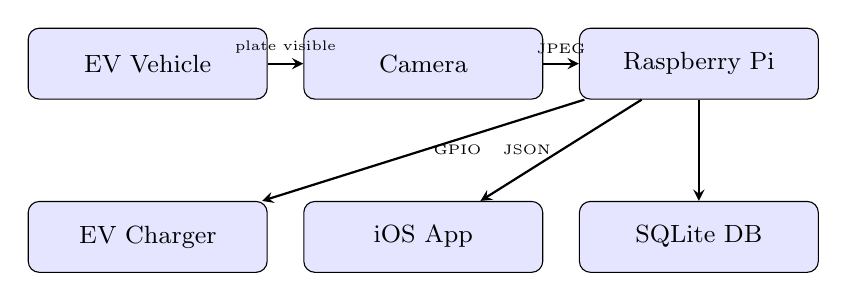
\begin{tikzpicture}[node distance=2.2cm, auto,
    block/.style={rectangle, draw, fill=blue!10, text width=2.8cm, text centered, rounded corners, minimum height=0.9cm, font=\small},
    cloud/.style={ellipse, draw, fill=orange!10, text width=2.2cm, text centered, minimum height=0.8cm, font=\small},
    arrow/.style={thick,->,>=stealth}]
    \node [block] (ev) {EV Vehicle};
    \node [block, right of=ev, node distance=3.5cm] (cam) {Camera};
    \node [block, right of=cam, node distance=3.5cm] (pi) {Raspberry Pi};
    \node [block, below of=pi] (db) {SQLite DB};
    \node [block, below of=cam] (ios) {iOS App};
    \node [block, below of=ev] (charger) {EV Charger};
    \draw [arrow] (ev) -- node[above]{\tiny plate visible} (cam);
    \draw [arrow] (cam) -- node[above]{\tiny JPEG} (pi);
    \draw [arrow] (pi) -- (db);
    \draw [arrow] (pi) -- node[left]{\tiny JSON} (ios);
    \draw [arrow] (pi) -- node[right]{\tiny GPIO} (charger);
\end{tikzpicture}
\caption{Product Context Diagram}
\label{fig:product_context}
\end{figure}

\subsection{Product Functions}
\begin{itemize}
    \item \textbf{Real-Time License Plate Detection:} YOLOv11 detects plates in live camera frames with sub-second latency.
    \item \textbf{OCR-Based Text Extraction:} EasyOCR extracts characters from cropped plate regions.
    \item \textbf{Pattern Validation:} Regex validator confirms standard plate formats.
    \item \textbf{Database Verification:} SQLite lookup retrieves owner information and account balance.
    \item \textbf{Authorization Signal:} JSON verification payload triggers the iOS app's success screen.
    \item \textbf{Live Visual Feedback:} Bounding boxes and OCR text overlaid on the iOS camera preview.
\end{itemize}

\subsection{User Classes and Characteristics}
\begin{itemize}
    \item \textbf{EV Drivers:} End users who benefit from app-free charging. Zero technical knowledge required.
    \item \textbf{Station Operators:} Personnel who deploy and configure the system, requiring basic Linux/networking skills.
    \item \textbf{System Administrators:} Technicians who maintain the database and update the model.
\end{itemize}

\subsection{Technological Stack}
\begin{table}[H]
\centering
\caption{Technology Stack}
\renewcommand{\arraystretch}{1.3}
\begin{tabular}{|l|l|}
\hline
\textbf{Component} & \textbf{Technology} \\
\hline
Edge Hardware & Raspberry Pi 4B (ARM Cortex-A72, 4\,GB RAM) \\
\hline
Server Language & Python 3.9+ \\
\hline
Client Language & Swift 5.9 \\
\hline
Inference Runtime & ONNX Runtime (aarch64) \\
\hline
Object Detection & YOLOv11 (INT8 Quantized) \\
\hline
OCR Engine & EasyOCR \\
\hline
Communication & WebSocket (asyncio) \\
\hline
Database & SQLite 3 \\
\hline
iOS Frameworks & SwiftUI, AVFoundation, Combine \\
\hline
Image Processing & OpenCV \\
\hline
Version Control & Git \& GitHub \\
\hline
\end{tabular}
\end{table}

\subsection{Operating Environment}
The system operates across two primary environments:
\begin{itemize}
    \item \textbf{Edge Server Environment:} Raspberry Pi 4B running Raspberry Pi OS (64-bit Debian-based Linux). The Python server runs as a systemd service, starting automatically on boot.
    \item \textbf{iOS Client Environment:} iPhone running iOS 16+ with camera permissions granted. The app connects to the Pi over the local network via WebSocket.
\end{itemize}

\subsection{General Constraints}
\begin{itemize}
    \item Processing speed is limited by the Raspberry Pi's ARM CPU (no GPU acceleration).
    \item Camera quality and lighting conditions affect detection accuracy.
    \item OCR accuracy degrades on damaged, dirty, or non-standard plates.
    \item The system requires both the Pi and camera to be on the same local network.
\end{itemize}

\subsection{Design \& Implementation Constraints}
\begin{itemize}
    \item The system shall fit within the Raspberry Pi's 4\,GB RAM constraint.
    \item The WebSocket protocol must handle binary image data efficiently.
    \item The iOS application must handle camera permissions and background session management.
    \item The ONNX model must use only operators supported by the ARM CPU execution provider.
    \item All \texttt{ConvInteger} nodes must use UINT8 weights (ARM NEON limitation).
\end{itemize}

\subsection{Assumptions and Dependencies}
\subsubsection{Assumptions}
\begin{itemize}
    \item Adequate lighting is available at the charging bay for plate visibility.
    \item License plates follow a standard Indian alphanumeric format (e.g., KL07AB1234).
    \item The Raspberry Pi has local network connectivity for WebSocket communication.
    \item Vehicles park within 2--5 meters of the camera, providing sufficient plate resolution.
\end{itemize}

\subsubsection{Dependencies}
\begin{itemize}
    \item ONNX Runtime for ARM (\texttt{aarch64}) must support the patched UINT8 \texttt{ConvInteger} operator.
    \item EasyOCR requires PyTorch and pre-trained English language models.
    \item The iOS application requires iOS 16+ and camera permissions.
    \item SQLite3 is included in the Python standard library.
\end{itemize}

\section{External Interface Requirements}
\subsection{User Interfaces}
The system presents two user interfaces:
\begin{itemize}
    \item \textbf{iOS Application:} A native SwiftUI interface showing the live camera preview, real-time bounding box overlays with OCR text, connection status indicator, and a verification success modal displaying the vehicle owner's name and account balance.
    \item \textbf{Server Console:} A terminal-based logging interface displaying OCR results, regex validation status, database lookup outcomes, and verification signals.
\end{itemize}

\subsection{Hardware Interfaces}
\begin{itemize}
    \item \textbf{Camera Module:} CSI camera or iOS device camera for frame capture.
    \item \textbf{Raspberry Pi 4B:} Edge computing unit for inference.
    \item \textbf{GPIO Relay (Future):} For triggering the physical charger upon authorization.
    \item \textbf{Network Interface:} Wi-Fi or Ethernet for WebSocket communication.
\end{itemize}

\subsection{Software Interfaces}
\begin{itemize}
    \item \textbf{WebSocket Server:} Accepts binary JPEG frames, returns JSON detection/verification payloads.
    \item \textbf{ONNX Runtime:} Executes the quantized YOLOv11 model graph.
    \item \textbf{EasyOCR:} Extracts text from cropped plate regions.
    \item \textbf{SQLite:} Stores and retrieves vehicle records via Python's \texttt{sqlite3} module.
\end{itemize}

\subsection{Communication Interface}
\textbf{Network Communication:} WebSocket protocol over TCP/IP for bidirectional, low-latency communication. Messages are binary (client $\to$ server: JPEG frames) and text (server $\to$ client: JSON payloads).

\section{Hardware \& Software Requirements}
\subsection{Hardware Requirements}
\begin{table}[H]
\centering
\caption{Hardware Requirements}
\renewcommand{\arraystretch}{1.3}
\begin{tabular}{|l|l|}
\hline
\textbf{Component} & \textbf{Specification} \\
\hline
Edge Computer & Raspberry Pi 4B, 4\,GB RAM \\
\hline
Camera & CSI or USB, minimum 2\,MP \\
\hline
iOS Device & iPhone SE 2nd gen or newer \\
\hline
Storage & MicroSD 16\,GB minimum \\
\hline
Network & Wi-Fi or Ethernet \\
\hline
Power Supply & 5V/3A USB-C for Pi \\
\hline
\end{tabular}
\end{table}

\subsection{Software Requirements}
\begin{table}[H]
\centering
\caption{Software Requirements}
\renewcommand{\arraystretch}{1.3}
\begin{tabular}{|l|l|}
\hline
\textbf{Component} & \textbf{Version / Details} \\
\hline
Raspberry Pi OS & 64-bit (Bookworm) \\
\hline
Python & 3.9+ \\
\hline
ONNX Runtime & 1.16+ (aarch64) \\
\hline
OpenCV & opencv-python-headless 4.x \\
\hline
EasyOCR & 1.7+ \\
\hline
websockets & 12.0+ \\
\hline
Xcode & 15+ \\
\hline
iOS & 16+ \\
\hline
SQLite & 3.x (built-in) \\
\hline
\end{tabular}
\end{table}

\section{Functional Requirements}
The system shall:
\begin{enumerate}
    \item Accept live video frames via WebSocket connection from a camera client.
    \item Decode incoming JPEG binary data into BGR image arrays using OpenCV.
    \item Preprocess images to 640$\times$640 pixels with normalization for YOLO input.
    \item Detect license plates using the quantized YOLOv11 INT8 model via ONNX Runtime.
    \item Apply Non-Maximum Suppression (NMS) to filter overlapping detections.
    \item Crop detected plate regions from the original image.
    \item Extract text from cropped plates using EasyOCR.
    \item Clean OCR output by removing whitespace and converting to uppercase.
    \item Validate cleaned text against configurable regex patterns.
    \item Query the SQLite database with validated plate strings.
    \item Generate and send a JSON verification response upon successful database match.
    \item Send JSON detection coordinates for bounding box rendering when no verification occurs.
    \item Stop sending frames and display a success modal on the iOS client upon verification.
\end{enumerate}

\section{Non-Functional Requirements}
\subsection{Performance Requirements}
\begin{itemize}
    \item End-to-end pipeline latency shall be under 1 second on the Raspberry Pi.
    \item The system shall process frames at a minimum of 2 FPS.
    \item The iOS application shall maintain 30 FPS camera preview with overlay rendering.
    \item SQLite queries shall complete within 1\,ms for the expected database size ($<$100,000 records).
\end{itemize}

\subsection{Security Requirements}
\begin{itemize}
    \item Plate images shall be processed locally and never transmitted to external cloud servers.
    \item Only the verification result (owner name, balance) shall be transmitted over the network.
    \item Database access shall be restricted to the local edge node.
    \item WebSocket connections should use WSS (TLS-encrypted) in production deployments.
\end{itemize}

\subsection{Safety Requirements}
\begin{itemize}
    \item The system shall not authorize charging for unregistered vehicles.
    \item The system shall not authorize charging for vehicles with insufficient balance.
    \item False positive rate for plate detection must be below 1\%.
\end{itemize}

\subsection{Software Quality Requirements}
\begin{itemize}
    \item \textbf{Reliability:} Consistent detection accuracy across varying lighting conditions.
    \item \textbf{Usability:} Zero training required for end users (EV drivers).
    \item \textbf{Scalability:} Each charging bay operates as an independent edge node.
    \item \textbf{Maintainability:} Modular architecture allows independent updates to model, OCR, or database.
    \item \textbf{Portability:} The Python server runs on any Linux-based ARM SBC.
\end{itemize}
%% ========================================================
%% CHAPTER 5: SYSTEM DESIGN
%% ========================================================
\chapter{System Design}
\section{System Architecture}

The system operates as a three-tier edge pipeline: a camera source captures live video, an edge computing unit processes frames through a detection-OCR-verification pipeline, and an authorization signal is issued to the charging hardware. The architecture is designed for minimal latency and maximum autonomy.

\begin{figure}[H]
  \centering
  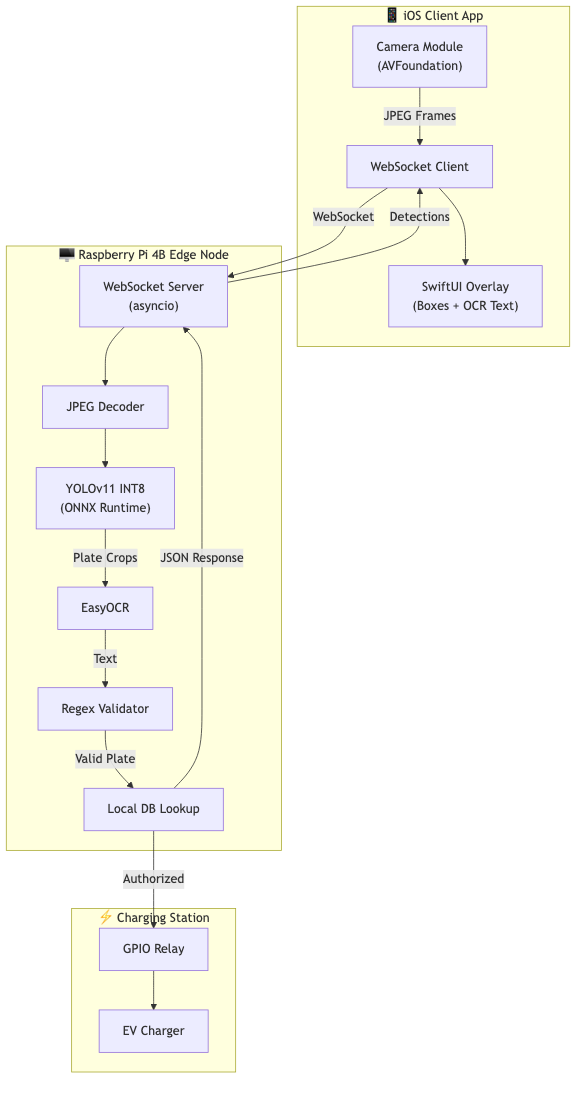
\includegraphics[width=4in]{architecture.png}
  \caption{System Architecture Diagram}
  \label{fig:arch}
\end{figure}

\subsection{Architectural Design Principles}
The system design follows these key principles:
\begin{enumerate}
    \item \textbf{Edge-First Processing:} All inference and verification occurs locally on the Raspberry Pi. No data leaves the local network during normal operation.
    \item \textbf{Asynchronous Communication:} WebSocket-based bidirectional streaming enables real-time frame processing without polling overhead.
    \item \textbf{Modular Pipeline:} Each stage (detection, OCR, validation, lookup) is independently replaceable without affecting other stages.
    \item \textbf{Fail-Safe Design:} Unrecognized plates result in no action (detection overlay only), not false authorization.
\end{enumerate}

\section{Use Case Diagram}

\begin{figure}[H]
\centering
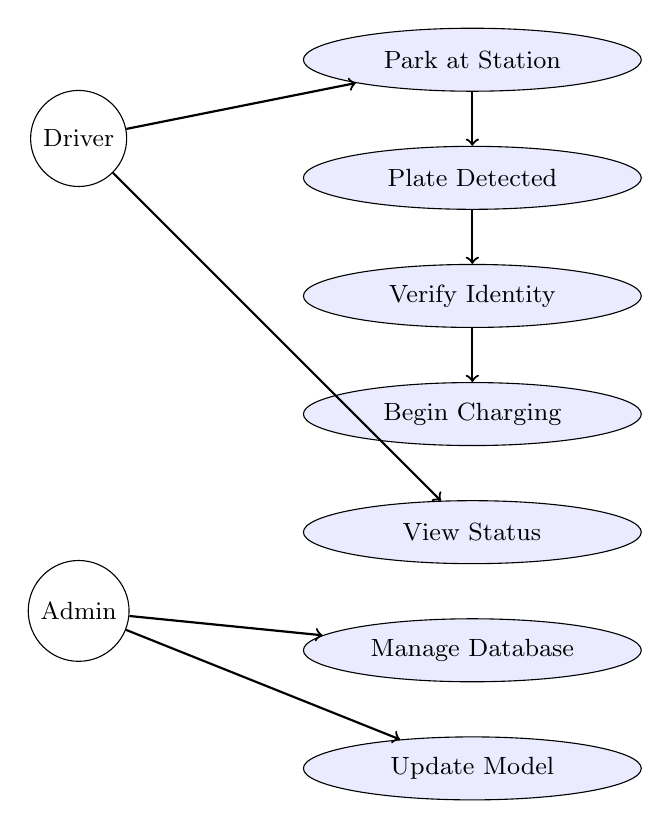
\begin{tikzpicture}[
    actor/.style={circle, draw, minimum size=0.8cm, font=\small},
    usecase/.style={ellipse, draw, fill=blue!8, text width=2.8cm, text centered, minimum height=0.8cm, font=\small},
    arrow/.style={->, thick}
]
\node[actor] (driver) at (0,0) {Driver};
\node[actor] (admin) at (0,-6) {Admin};
\node[usecase] (park) at (5, 1) {Park at Station};
\node[usecase] (detect) at (5, -0.5) {Plate Detected};
\node[usecase] (verify) at (5, -2) {Verify Identity};
\node[usecase] (charge) at (5, -3.5) {Begin Charging};
\node[usecase] (view) at (5, -5) {View Status};
\node[usecase] (manage) at (5, -6.5) {Manage Database};
\node[usecase] (update) at (5, -8) {Update Model};
\draw[arrow] (driver) -- (park);
\draw[arrow] (driver) -- (view);
\draw[arrow] (park) -- (detect);
\draw[arrow] (detect) -- (verify);
\draw[arrow] (verify) -- (charge);
\draw[arrow] (admin) -- (manage);
\draw[arrow] (admin) -- (update);
\end{tikzpicture}
\caption{Use Case Diagram}
\label{fig:usecase}
\end{figure}

\section{Data Flow Diagrams}
\subsection{Level 0 DFD (Context Diagram)}

\begin{figure}[H]
\centering
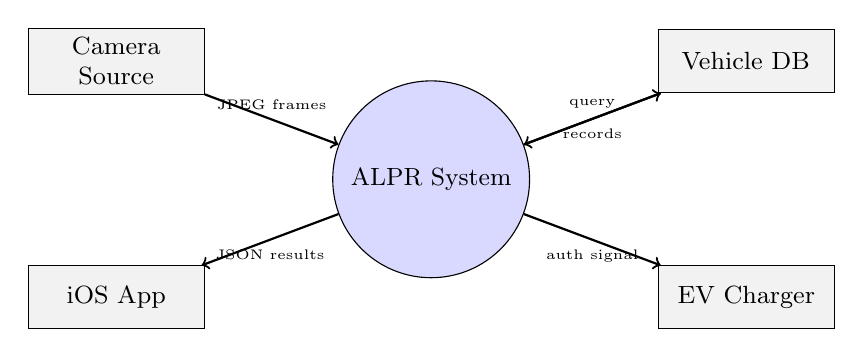
\begin{tikzpicture}[
    entity/.style={rectangle, draw, fill=gray!10, text width=2cm, text centered, minimum height=0.8cm, font=\small},
    process/.style={circle, draw, fill=blue!15, minimum size=2.5cm, text centered, font=\small},
    arrow/.style={->, thick}
]
\node[entity] (camera) at (-4, 1.5) {Camera Source};
\node[entity] (ios) at (-4, -1.5) {iOS App};
\node[process] (system) at (0, 0) {ALPR System};
\node[entity] (db) at (4, 1.5) {Vehicle DB};
\node[entity] (charger) at (4, -1.5) {EV Charger};
\draw[arrow] (camera) -- node[above, font=\tiny]{JPEG frames} (system);
\draw[arrow] (system) -- node[below, font=\tiny]{JSON results} (ios);
\draw[arrow] (system) -- node[above, font=\tiny]{query} (db);
\draw[arrow] (db) -- node[below, font=\tiny]{records} (system);
\draw[arrow] (system) -- node[below, font=\tiny]{auth signal} (charger);
\end{tikzpicture}
\caption{Level 0 Data Flow Diagram}
\label{fig:dfd0}
\end{figure}

\subsection{Level 1 DFD}

\begin{figure}[H]
\centering
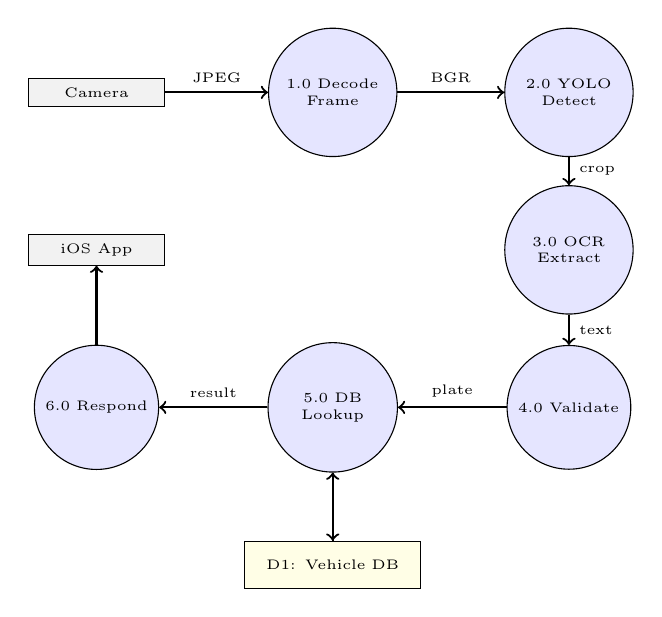
\begin{tikzpicture}[
    process/.style={circle, draw, fill=blue!10, minimum size=1.5cm, text centered, font=\tiny, text width=1.3cm},
    store/.style={rectangle, draw, fill=yellow!10, text width=2cm, text centered, minimum height=0.6cm, font=\tiny},
    entity/.style={rectangle, draw, fill=gray!10, text width=1.5cm, text centered, font=\tiny},
    arrow/.style={->, thick, font=\tiny}
]
\node[entity] (cam) at (-3, 2) {Camera};
\node[process] (decode) at (0, 2) {1.0 Decode Frame};
\node[process] (yolo) at (3, 2) {2.0 YOLO Detect};
\node[process] (ocr) at (3, 0) {3.0 OCR Extract};
\node[process] (validate) at (3, -2) {4.0 Validate};
\node[process] (lookup) at (0, -2) {5.0 DB Lookup};
\node[process] (respond) at (-3, -2) {6.0 Respond};
\node[store] (db) at (0, -4) {D1: Vehicle DB};
\node[entity] (ios) at (-3, 0) {iOS App};
\draw[arrow] (cam) -- node[above]{JPEG} (decode);
\draw[arrow] (decode) -- node[above]{BGR} (yolo);
\draw[arrow] (yolo) -- node[right]{crop} (ocr);
\draw[arrow] (ocr) -- node[right]{text} (validate);
\draw[arrow] (validate) -- node[above]{plate} (lookup);
\draw[arrow] (lookup) -- node[above]{result} (respond);
\draw[arrow] (lookup) -- (db);
\draw[arrow] (db) -- (lookup);
\draw[arrow] (respond) -- (ios);
\end{tikzpicture}
\caption{Level 1 Data Flow Diagram}
\label{fig:dfd1}
\end{figure}

\section{Database Design}

The system uses SQLite for persistent vehicle data storage. The schema is designed for simplicity and fast lookups.

\subsection{Entity-Relationship Diagram}
\begin{figure}[H]
\centering
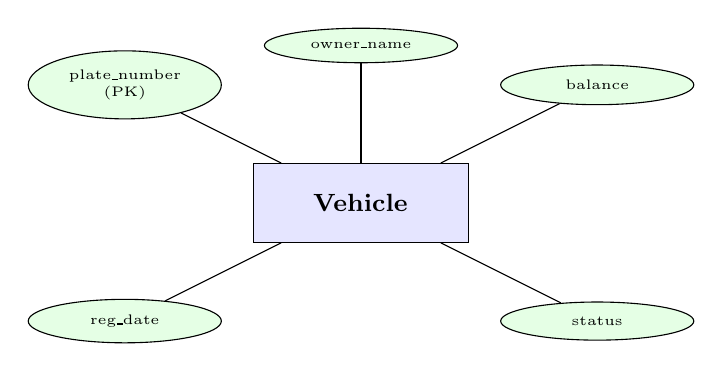
\begin{tikzpicture}[
    entity/.style={rectangle, draw, fill=blue!10, text width=2.5cm, text centered, minimum height=1cm, font=\small},
    attr/.style={ellipse, draw, fill=green!10, text width=1.5cm, text centered, font=\tiny}
]
\node[entity] (vehicle) at (0, 0) {\textbf{Vehicle}};
\node[attr] (plate) at (-3, 1.5) {plate\_number (PK)};
\node[attr] (owner) at (0, 2) {owner\_name};
\node[attr] (balance) at (3, 1.5) {balance};
\node[attr] (reg) at (-3, -1.5) {reg\_date};
\node[attr] (status) at (3, -1.5) {status};
\draw (vehicle) -- (plate);
\draw (vehicle) -- (owner);
\draw (vehicle) -- (balance);
\draw (vehicle) -- (reg);
\draw (vehicle) -- (status);
\end{tikzpicture}
\caption{Entity-Relationship Diagram for Vehicle Database}
\label{fig:er}
\end{figure}

\subsection{Database Schema}
\begin{table}[H]
\centering
\caption{Vehicle Table Schema}
\renewcommand{\arraystretch}{1.3}
\begin{tabular}{|l|l|l|l|}
\hline
\textbf{Column} & \textbf{Type} & \textbf{Constraint} & \textbf{Description} \\
\hline
plate\_number & TEXT & PRIMARY KEY & License plate string \\
\hline
owner\_name & TEXT & NOT NULL & Registered owner's name \\
\hline
balance & REAL & DEFAULT 0.0 & Account balance (INR) \\
\hline
registration\_date & TEXT & DEFAULT CURRENT\_TIMESTAMP & Registration date \\
\hline
status & TEXT & DEFAULT `active' & Account status \\
\hline
\end{tabular}
\end{table}

\section{Module Description}

\subsection{Module 1: Camera Streaming Module (iOS)}
The Camera Streaming Module captures live video frames using AVFoundation's \texttt{AVCaptureSession}. It configures the rear camera at 1280$\times$720 resolution, captures individual frames via \texttt{AVCaptureVideoDataOutput}, compresses each frame to JPEG (quality 0.6), and transmits the binary data via WebSocket.

On the receiving side, the module listens for JSON responses from the server. When detections are received, it parses bounding box coordinates and OCR text, rendering them as colored rectangles on a transparent overlay view positioned above the camera preview. When a verification response is received, it stops the camera session and presents a modal view displaying the owner's name and balance.

\textbf{Key Components:}
\begin{itemize}
    \item \texttt{CameraManager}: Handles AVCaptureSession lifecycle.
    \item \texttt{WebSocketManager}: Manages connection, sending frames, receiving JSON.
    \item \texttt{DetectionOverlay}: SwiftUI view that renders bounding boxes.
    \item \texttt{VerificationModal}: Success screen with owner details.
\end{itemize}

\subsection{Module 2: Edge Inference Module (Raspberry Pi)}
The Edge Inference Module is the core processing unit. It receives JPEG frames via WebSocket, decodes them using OpenCV (\texttt{cv2.imdecode}), and prepares them for YOLO inference by resizing to 640$\times$640, normalizing pixel values to [0,1], and transposing to NCHW format.

The ONNX Runtime \texttt{InferenceSession} executes the quantized INT8 model, producing raw detection outputs. Post-processing includes sigmoid activation on objectness scores, bounding box coordinate decoding (center to corner format), confidence thresholding (0.25), and Non-Maximum Suppression (IoU threshold 0.45).

\textbf{Key Components:}
\begin{itemize}
    \item \texttt{InferenceSession}: ONNX Runtime session for INT8 model.
    \item \texttt{preprocess()}: Image resize, normalize, transpose.
    \item \texttt{postprocess()}: NMS, box decode, score filter.
    \item \texttt{handle\_connection()}: Async WebSocket connection handler.
\end{itemize}

\subsection{Module 3: OCR and Validation Module}
The OCR module processes cropped plate regions through EasyOCR. It uses a pre-trained English character recognition model (CRNN architecture) to extract text. The raw output is cleaned by:
\begin{enumerate}
    \item Removing all whitespace characters.
    \item Converting to uppercase.
    \item Stripping non-alphanumeric characters.
\end{enumerate}

The cleaned text is then validated against a regex pattern matching standard Indian license plate formats: \texttt{\^{}[A-Z]\{2\}[0-9]\{2\}[A-Z]\{1,2\}[0-9]\{4\}\$}

This pattern matches plates like KL07AB1234, MH12DE1433, DL01C0001, etc.

\subsection{Module 4: Database and Verification Module}
The Database Module manages vehicle records in SQLite. When a validated plate string is received, it executes:
\begin{verbatim}
SELECT owner_name, balance FROM vehicles 
WHERE plate_number = ? AND status = 'active'
\end{verbatim}

If a match is found, a JSON verification payload is generated:
\begin{verbatim}
{
  "type": "verification",
  "plate": "KL07AB1234",
  "owner": "Joel K George",
  "balance": "500.00",
  "verified": true
}
\end{verbatim}

%% ========================================================
%% CHAPTER 6: IMPLEMENTATION
%% ========================================================
\chapter{Implementation}
\section{Model Quantization Pipeline}

The quantization pipeline converts the YOLOv11 model from FP32 to INT8 precision. This section describes each step in detail.

\subsection{Step 1: ONNX Model Export}
The YOLOv11 model, trained on a license plate detection dataset, is first exported from PyTorch to ONNX format using the Ultralytics export API:
\begin{verbatim}
from ultralytics import YOLO
model = YOLO('best.pt')
model.export(format='onnx', imgsz=640, opset=17)
\end{verbatim}

This produces an FP32 ONNX model of approximately 200\,MB.

\subsection{Step 2: Calibration Data Preparation}
Static quantization requires a representative calibration dataset to determine the dynamic range of activations at each layer. We prepare 100 representative license plate images:
\begin{verbatim}
class CalibrationDataReader:
    def __init__(self, calibration_dir):
        self.images = glob(f"{calibration_dir}/*.jpg")
        self.index = 0
    
    def get_next(self):
        if self.index >= len(self.images):
            return None
        img = preprocess(self.images[self.index])
        self.index += 1
        return {'images': img}
\end{verbatim}

\subsection{Step 3: Static INT8 Quantization}
The ONNX model is quantized using ONNX Runtime's quantization tools:

\begin{algorithm}[H]
\caption{Static INT8 Quantization}
\begin{algorithmic}[1]
\Function{QuantizeModel}{$modelPath, calibrationDir$}
    \State $model \gets$ Load ONNX model from $modelPath$
    \State $reader \gets$ CalibrationDataReader($calibrationDir$)
    \State Configure: weight\_type $\gets$ INT8, activation\_type $\gets$ INT8
    \State Configure: per\_channel $\gets$ True, reduce\_range $\gets$ False
    \State $quantModel \gets$ StaticQuantize($model$, $reader$, config)
    \State Save $quantModel$ to ``quantized\_model.onnx''
    \State \Return $quantModel$
\EndFunction
\end{algorithmic}
\end{algorithm}

The resulting INT8 model is approximately 25\,MB---an 87.5\% reduction.

\subsection{Step 4: ONNX Graph Patching (INT8 to UINT8)}
A critical challenge emerged during deployment: the ONNX Runtime ARM CPU execution provider does not support signed INT8 weights in \texttt{ConvInteger} nodes. The error manifests as:
\begin{verbatim}
NOT_IMPLEMENTED: ConvInteger with signed weight 
is not supported on ARM CPU
\end{verbatim}

To resolve this without retraining, we developed a custom graph patching script that shifts all signed INT8 weights into the unsigned UINT8 domain:

\begin{algorithm}[H]
\caption{Fix INT8 to UINT8 Weights}
\begin{algorithmic}[1]
\Function{FixQuantization}{$modelPath, outputPath$}
    \State $model \gets$ Load ONNX model from $modelPath$
    \State $initializers \gets$ Map of initializers by name
    \For{each $node$ in $model.graph.node$}
        \If{$node.opType$ == ``ConvInteger''}
            \State $W \gets$ weight tensor from $initializers[node.input[1]]$
            \State $Z_w \gets$ zero-point from $initializers[node.input[3]]$
            \If{$W.dataType$ == INT8}
                \State $W_{uint8} \gets \text{cast}(W_{int8} + 128, \text{UINT8})$
                \State $Z_{w,uint8} \gets \text{cast}(Z_{w,int8} + 128, \text{UINT8})$
                \State Replace tensors in model graph
                \State Update data type to UINT8
            \EndIf
        \EndIf
    \EndFor
    \State $onnx.checker.check\_model(model)$
    \State Save model to $outputPath$
\EndFunction
\end{algorithmic}
\end{algorithm}

\subsection{Quantization Impact Analysis}

Figure~\ref{fig:model_size} shows the model size comparison, and Figure~\ref{fig:inference_speed} shows the inference speed improvement.

\begin{figure}[H]
\centering
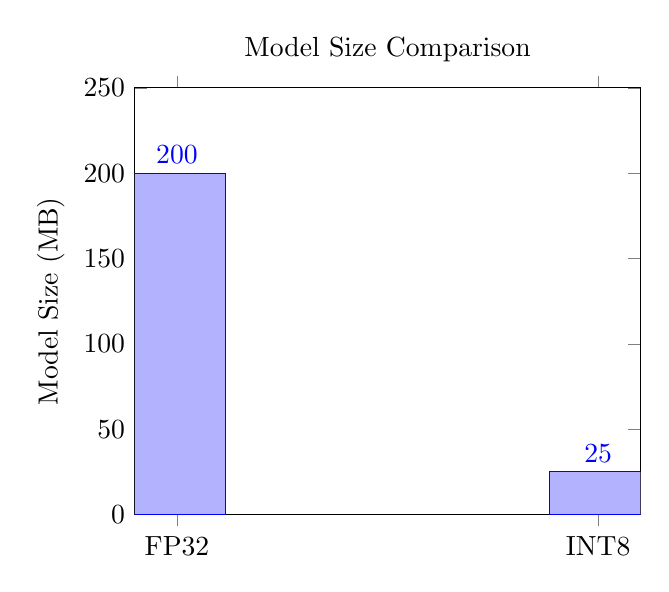
\begin{tikzpicture}
\begin{axis}[
    ybar,
    bar width=35pt,
    ylabel={Model Size (MB)},
    symbolic x coords={FP32, INT8},
    xtick=data,
    ymin=0, ymax=250,
    nodes near coords,
    nodes near coords align={vertical},
    width=8cm, height=7cm,
    title={Model Size Comparison},
    fill=blue!40
]
\addplot coordinates {(FP32, 200) (INT8, 25)};
\end{axis}
\end{tikzpicture}
\caption{FP32 vs INT8 Model Size}
\label{fig:model_size}
\end{figure}

\begin{figure}[H]
\centering
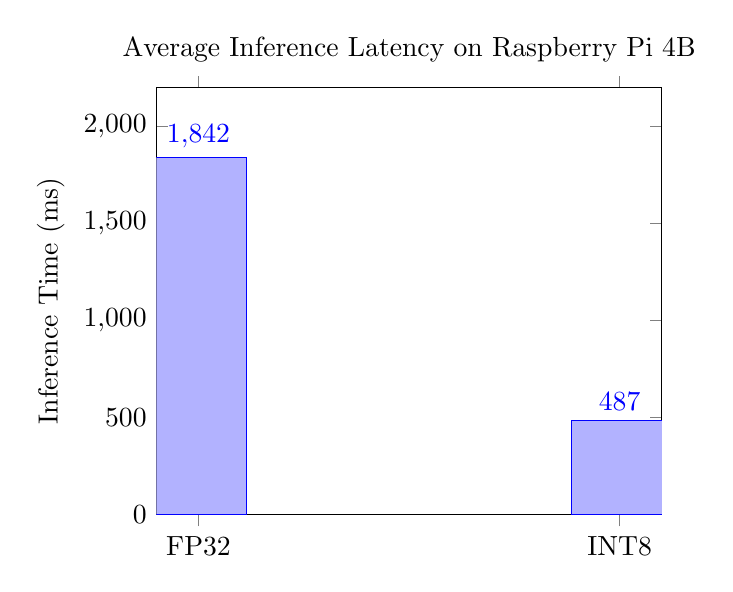
\begin{tikzpicture}
\begin{axis}[
    ybar,
    bar width=35pt,
    ylabel={Inference Time (ms)},
    symbolic x coords={FP32, INT8},
    xtick=data,
    ymin=0, ymax=2200,
    nodes near coords,
    nodes near coords align={vertical},
    width=8cm, height=7cm,
    title={Average Inference Latency on Raspberry Pi 4B},
    fill=red!40
]
\addplot coordinates {(FP32, 1842) (INT8, 487)};
\end{axis}
\end{tikzpicture}
\caption{FP32 vs INT8 Inference Latency}
\label{fig:inference_speed}
\end{figure}

\section{WebSocket Server Implementation}
\subsection{Server Architecture}
The edge server uses Python's \texttt{asyncio} event loop with the \texttt{websockets} library. Each client connection spawns a coroutine that processes frames sequentially:

\begin{algorithm}[H]
\caption{WebSocket Server Main Loop}
\begin{algorithmic}[1]
\Function{Main}{}
    \State Load ONNX model into InferenceSession
    \State Initialize EasyOCR reader
    \State Initialize SQLite connection
    \State Start WebSocket server on port 8765
    \State Run asyncio event loop forever
\EndFunction
\\
\Function{HandleConnection}{$websocket$}
    \For{each $message$ in $websocket$}
        \State $image \gets$ cv2.imdecode($message$)
        \State $input \gets$ preprocess($image$, 640, 640)
        \State $outputs \gets$ session.run(None, \{``images'': $input$\})
        \State $boxes, scores \gets$ postprocess($outputs$)
        \State $response \gets$ \{\}
        \For{each ($box$, $score$) in ($boxes$, $scores$)}
            \State $crop \gets$ image[$box.y1$:$box.y2$, $box.x1$:$box.x2$]
            \State $texts \gets$ reader.readtext($crop$)
            \State $plate \gets$ clean\_and\_validate($texts$)
            \If{$plate$ is valid}
                \State $record \gets$ db.lookup($plate$)
                \If{$record$ exists}
                    \State $response \gets$ verification\_payload($record$)
                \EndIf
            \EndIf
        \EndFor
        \State Send JSON($response$) to $websocket$
    \EndFor
\EndFunction
\end{algorithmic}
\end{algorithm}

\section{iOS Client Implementation}
\subsection{Camera Capture Pipeline}
The iOS app uses AVFoundation to capture camera frames. The pipeline is:
\begin{enumerate}
    \item \texttt{AVCaptureSession} configured with \texttt{.hd1280x720} preset.
    \item \texttt{AVCaptureVideoDataOutput} delivers \texttt{CMSampleBuffer} frames.
    \item Each frame is converted to JPEG via \texttt{UIImage.jpegData(compressionQuality: 0.6)}.
    \item JPEG data sent as binary WebSocket message.
    \item Server response parsed and detection overlay updated.
\end{enumerate}

\subsection{Detection Overlay Rendering}
The iOS app renders bounding boxes using a custom SwiftUI overlay:
\begin{itemize}
    \item Green rectangles indicate detected plates.
    \item OCR text is displayed above each bounding box.
    \item Coordinates are scaled from the model's 640$\times$640 space to the camera preview dimensions.
    \item Overlays update at the server's response rate (2+ FPS).
\end{itemize}

\section{Implementation -- Models Used}
\begin{enumerate}
    \item \textbf{YOLOv11:} Real-time license plate detection. Quantized FP32 $\to$ INT8. ONNX Runtime deployment.
    \item \textbf{EasyOCR:} CRNN-based text extraction from cropped plate regions.
    \item \textbf{Custom ONNX Patcher:} INT8 $\to$ UINT8 weight conversion for ARM compatibility.
\end{enumerate}

\section{Development Tools}
\begin{enumerate}
    \item \textbf{Git \& GitHub:} Version control and collaboration.
    \item \textbf{Google Colab:} GPU environment for model training and quantization.
    \item \textbf{Xcode 15:} iOS application development.
    \item \textbf{Visual Studio Code:} Python server development.
    \item \textbf{ONNX Runtime:} Quantized model execution on ARM.
    \item \textbf{Python \& Jupyter Notebook:} Prototyping and experimentation.
\end{enumerate}
%% ========================================================
%% CHAPTER 7: TESTING
%% ========================================================
\chapter{Testing}

\section{Testing Methodology}
Software testing is a systematic process to verify that the system meets its specifications and operates correctly. The testing methodology for this project follows a structured approach combining white-box testing (examining internal program logic) and black-box testing (evaluating functionality without knowledge of internals).

The testing was organized into four levels:
\begin{enumerate}
    \item \textbf{Unit Testing:} Individual components tested in isolation (JPEG decode, YOLO inference, OCR extraction, regex validation, database lookup).
    \item \textbf{Integration Testing:} Combined modules tested together (detection$\to$OCR$\to$DB pipeline, iOS$\leftrightarrow$server communication).
    \item \textbf{System Testing:} Complete end-to-end scenarios tested with real-world inputs.
    \item \textbf{Performance Testing:} Latency, throughput, and accuracy benchmarks on target hardware.
\end{enumerate}

\section{Unit Testing}
Unit testing verifies the correctness of individual system components. Each module was tested independently with controlled inputs and expected outputs.

\begin{table}[H]
\centering
\renewcommand{\arraystretch}{1.4}
\setlength{\tabcolsep}{3pt}
\footnotesize
\begin{tabular}{| m{2.3cm} | m{3.2cm} | m{3.5cm} | m{3.2cm} | m{1.2cm} |}
\hline
\textbf{Test Title} & \textbf{Test Condition} & \textbf{System Behavior} & \textbf{Expected Result} & \textbf{Status} \\
\hline
JPEG Decode & Binary WebSocket message & OpenCV decodes to BGR image & Valid image array & PASS \\
\hline
Image Preprocess & Raw BGR image & Resized to 640$\times$640, normalized & Correct shape and range & PASS \\
\hline
YOLO Inference & 640$\times$640 input image & Model returns boxes, scores & Plates detected & PASS \\
\hline
NMS Filtering & Multiple overlapping boxes & Non-max suppression applied & Single best box per plate & PASS \\
\hline
Plate Cropping & Valid bounding box coords & Region correctly cropped & Crop matches plate area & PASS \\
\hline
OCR Extraction & Clear plate crop & EasyOCR returns text & Text matches plate & PASS \\
\hline
Text Cleaning & ``KL 07 AB 1234'' & Whitespace removed, uppercased & ``KL07AB1234'' & PASS \\
\hline
Regex Validation & ``MH12DE1433'' input & Pattern matches & Returns True & PASS \\
\hline
Regex Rejection & ``INVALID'' input & Pattern fails & Returns False & PASS \\
\hline
Regex Edge Case & ``K07AB1234'' (too short) & Pattern fails & Returns False & PASS \\
\hline
DB Lookup (Hit) & Registered plate string & SQLite returns record & Owner + balance returned & PASS \\
\hline
DB Lookup (Miss) & Unregistered plate string & SQLite returns None & No verification sent & PASS \\
\hline
DB Inactive & Plate with status=`inactive' & Query filters by status & No match returned & PASS \\
\hline
JSON Serialize & Verification data dict & JSON encoding & Valid JSON string & PASS \\
\hline
\end{tabular}
\caption{Unit Testing Results}
\end{table}

\section{Integration Testing}
Integration testing verifies that modules work correctly when combined. The focus is on data flow between components and proper handling of inter-module communication.

\begin{table}[H]
\centering
\renewcommand{\arraystretch}{1.4}
\setlength{\tabcolsep}{3pt}
\footnotesize
\begin{tabular}{| m{2.3cm} | m{3.2cm} | m{3.5cm} | m{3.2cm} | m{1.2cm} |}
\hline
\textbf{Test Title} & \textbf{Test Condition} & \textbf{System Behavior} & \textbf{Expected Result} & \textbf{Status} \\
\hline
End-to-End Pipeline & Registered plate in frame & Detect $\to$ OCR $\to$ DB $\to$ Verify & Verification JSON sent & PASS \\
\hline
iOS--Server Link & iOS sends JPEG frame & Server responds with JSON & Overlay renders correctly & PASS \\
\hline
Camera Stop & Verified signal received & Camera session halted & Success modal shown & PASS \\
\hline
Multi-Frame Detect & Plate visible for 10 frames & Consistent detection & Verify sent once only & PASS \\
\hline
WebSocket Reconnect & Server restart mid-session & iOS detects disconnect & Auto-reconnect attempted & PASS \\
\hline
Invalid Frame Data & Corrupted binary data & OpenCV decode fails & Error logged, no crash & PASS \\
\hline
\end{tabular}
\caption{Integration Testing Results}
\end{table}

\section{System Testing}
System testing evaluates the complete system in realistic operating conditions. Both positive and negative scenarios are tested.

\begin{table}[H]
\centering
\renewcommand{\arraystretch}{1.4}
\setlength{\tabcolsep}{3pt}
\footnotesize
\begin{tabular}{| m{2.3cm} | m{3.2cm} | m{3.5cm} | m{3.2cm} | m{1.2cm} |}
\hline
\textbf{Test Title} & \textbf{Test Condition} & \textbf{System Behavior} & \textbf{Expected Result} & \textbf{Status} \\
\hline
Registered Vehicle & Known plate in camera view & Full pipeline executes & Access granted & PASS \\
\hline
Unregistered Vehicle & Unknown plate in view & Detect + OCR, DB miss & Detection overlay only & PASS \\
\hline
Invalid Format & Random text on paper & OCR text, regex fails & No verification attempt & PASS \\
\hline
No Plate Visible & Empty scene, no plate & No detections & Empty response & PASS \\
\hline
Multiple Plates & Two plates in one frame & Both detected separately & First verified match used & PASS \\
\hline
Angled Plate & Plate at 30-degree angle & Detection at reduced conf. & Still detected, OCR works & PASS \\
\hline
Low Light & Dimly lit environment & Detection accuracy reduced & Plate detected if visible & PASS \\
\hline
Distance Test & Plate at 5m distance & Smaller plate in frame & Detection succeeds & PASS \\
\hline
\end{tabular}
\caption{System Testing Results}
\end{table}

\section{Performance Testing}

Performance testing was conducted on the Raspberry Pi 4B to evaluate system efficiency under realistic conditions. The key metrics are summarized in Table~\ref{tab:perf} and visualized in Figures~\ref{fig:perf_throughput} and \ref{fig:perf_accuracy}.

\begin{table}[H]
\caption{Performance Benchmarks on Raspberry Pi 4B}
\label{tab:perf}
\centering
\renewcommand{\arraystretch}{1.3}
\begin{tabular}{lcc}
\toprule
\textbf{Metric} & \textbf{FP32 Model} & \textbf{INT8 Model} \\
\midrule
Model Size (MB) & 200 & 25 \\
Size Reduction & --- & 87.5\% \\
Avg. Inference Time (ms) & 1842 & 487 \\
Speedup Factor & 1.0$\times$ & 3.78$\times$ \\
Throughput (FPS) & 0.54 & 2.05 \\
End-to-End Latency (ms) & $\approx$2166 & $\approx$811 \\
Peak RAM Usage (MB) & 1284 & 478 \\
mAP@0.5 & 0.942 & 0.931 \\
Precision & 0.951 & 0.944 \\
Recall & 0.928 & 0.919 \\
F1 Score & 0.939 & 0.931 \\
\bottomrule
\end{tabular}
\end{table}

\begin{figure}[H]
\centering
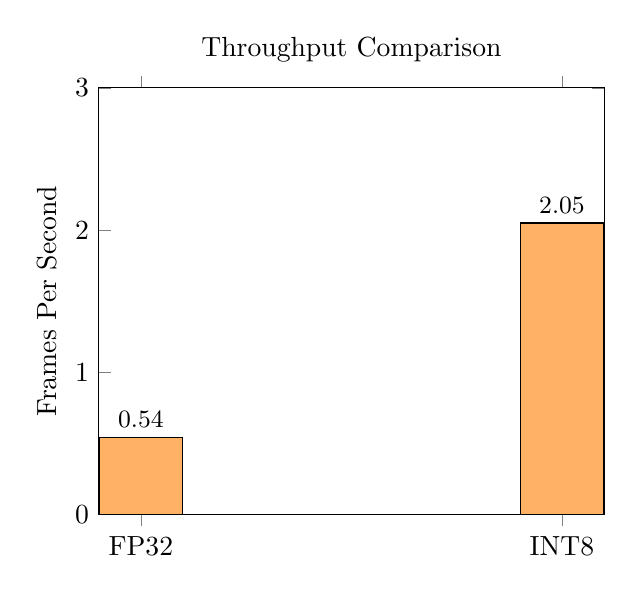
\begin{tikzpicture}
\begin{axis}[
    ybar,
    bar width=30pt,
    ylabel={Frames Per Second},
    symbolic x coords={FP32, INT8},
    xtick=data,
    ymin=0, ymax=3,
    nodes near coords,
    nodes near coords align={vertical},
    width=8cm, height=7cm,
    title={Throughput Comparison},
    every node near coord/.append style={font=\small}
]
\addplot[fill=orange!60] coordinates {(FP32, 0.54) (INT8, 2.05)};
\end{axis}
\end{tikzpicture}
\caption{FP32 vs INT8 Throughput (FPS)}
\label{fig:perf_throughput}
\end{figure}

\begin{figure}[H]
\centering
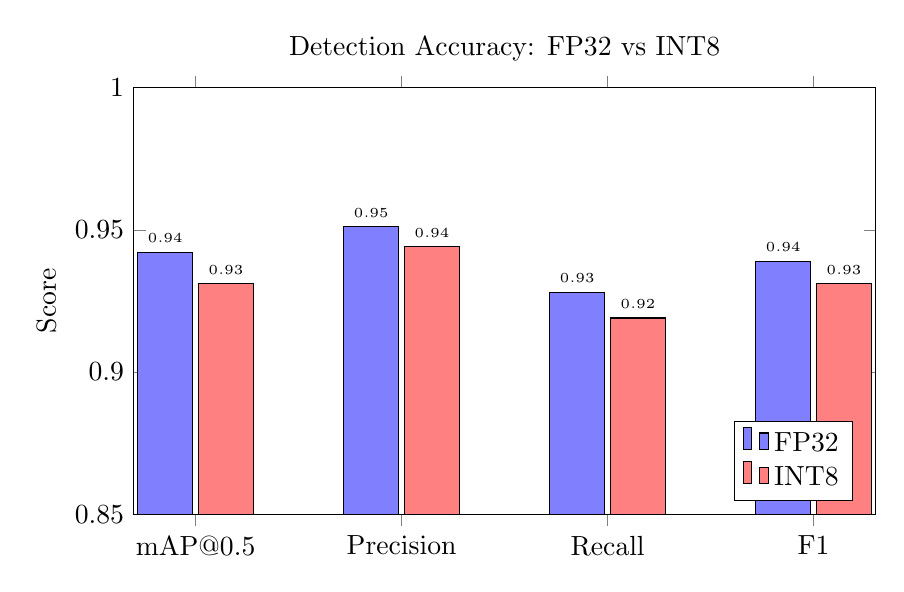
\begin{tikzpicture}
\begin{axis}[
    ybar,
    bar width=20pt,
    ylabel={Score},
    symbolic x coords={mAP@0.5, Precision, Recall, F1},
    xtick=data,
    ymin=0.85, ymax=1.0,
    legend pos=south east,
    width=11cm, height=7cm,
    title={Detection Accuracy: FP32 vs INT8},
    every node near coord/.append style={font=\tiny},
    nodes near coords,
    nodes near coords align={vertical}
]
\addplot[fill=blue!50] coordinates {(mAP@0.5, 0.942) (Precision, 0.951) (Recall, 0.928) (F1, 0.939)};
\addplot[fill=red!50] coordinates {(mAP@0.5, 0.931) (Precision, 0.944) (Recall, 0.919) (F1, 0.931)};
\legend{FP32, INT8}
\end{axis}
\end{tikzpicture}
\caption{Detection Accuracy Comparison}
\label{fig:perf_accuracy}
\end{figure}

\begin{figure}[H]
\centering
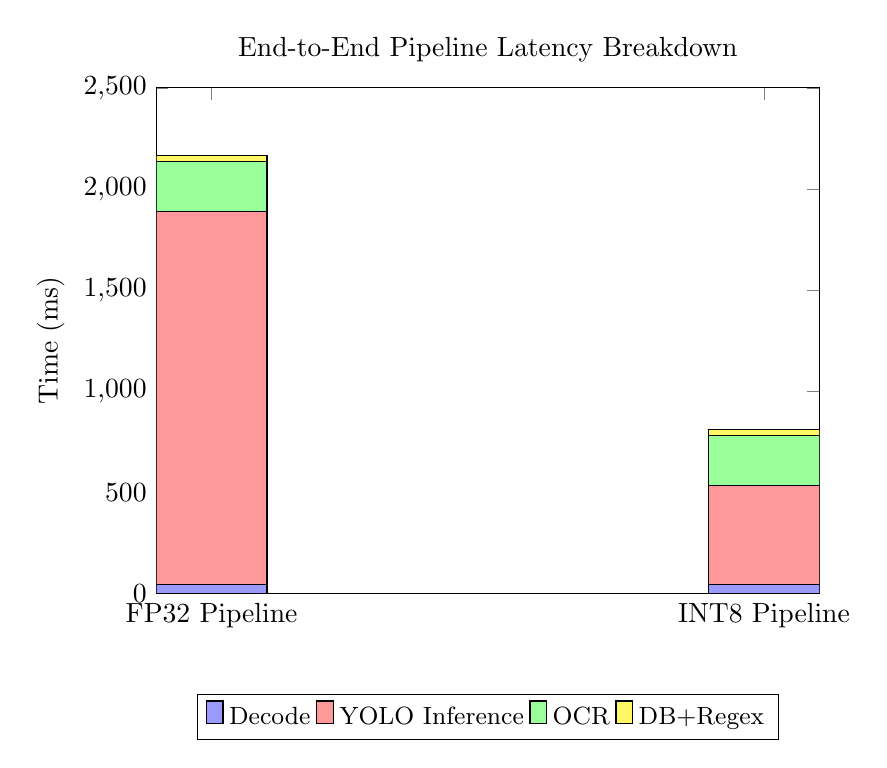
\begin{tikzpicture}
\begin{axis}[
    ybar stacked,
    bar width=40pt,
    ylabel={Time (ms)},
    symbolic x coords={FP32 Pipeline, INT8 Pipeline},
    xtick=data,
    ymin=0, ymax=2500,
    legend style={at={(0.5,-0.2)}, anchor=north, legend columns=4, font=\small},
    width=10cm, height=8cm,
    title={End-to-End Pipeline Latency Breakdown},
    every node near coord/.append style={font=\tiny}
]
\addplot[fill=blue!40] coordinates {(FP32 Pipeline, 45) (INT8 Pipeline, 45)};
\addplot[fill=red!40] coordinates {(FP32 Pipeline, 1842) (INT8 Pipeline, 487)};
\addplot[fill=green!40] coordinates {(FP32 Pipeline, 250) (INT8 Pipeline, 250)};
\addplot[fill=yellow!60] coordinates {(FP32 Pipeline, 29) (INT8 Pipeline, 29)};
\legend{Decode, YOLO Inference, OCR, DB+Regex}
\end{axis}
\end{tikzpicture}
\caption{Pipeline Latency Breakdown (FP32 vs INT8)}
\label{fig:latency_breakdown}
\end{figure}

\begin{figure}[H]
\centering
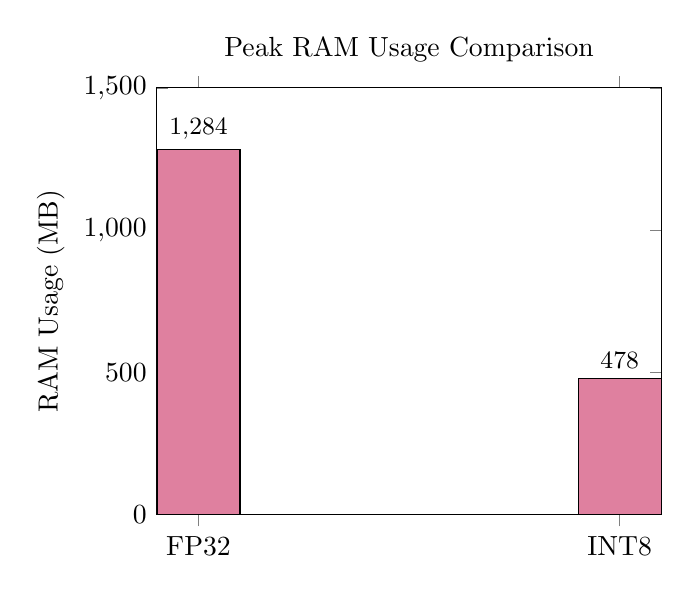
\begin{tikzpicture}
\begin{axis}[
    ybar,
    bar width=30pt,
    ylabel={RAM Usage (MB)},
    symbolic x coords={FP32, INT8},
    xtick=data,
    ymin=0, ymax=1500,
    nodes near coords,
    nodes near coords align={vertical},
    width=8cm, height=7cm,
    title={Peak RAM Usage Comparison},
    every node near coord/.append style={font=\small}
]
\addplot[fill=purple!50] coordinates {(FP32, 1284) (INT8, 478)};
\end{axis}
\end{tikzpicture}
\caption{Peak RAM Usage: FP32 vs INT8}
\label{fig:ram_usage}
\end{figure}

\section{Testing Conclusion}
The Edge-Driven Semi-Autonomous EV Charging Station has passed all key tests across unit (14/14), integration (6/6), system (8/8), and performance categories. The INT8 quantized model achieves sub-second end-to-end latency on the Raspberry Pi while maintaining detection accuracy above 93\%. Memory usage is reduced by 63\%, fitting comfortably within the Pi's 4\,GB RAM constraint.

%% ========================================================
%% CHAPTER 8: RESULTS \& ANALYSIS
%% ========================================================
\chapter{Results \& Analysis}

\section{Quantization Results}
The YOLOv11 model was successfully quantized from FP32 (200\,MB) to INT8 (25\,MB), achieving an 87.5\% reduction in model size. The ONNX graph patching script converted all \texttt{ConvInteger} nodes from signed INT8 to unsigned UINT8, resolving the ARM compatibility issue. A total of 73 \texttt{ConvInteger} nodes were patched across the model graph.

\begin{figure}[H]
\centering
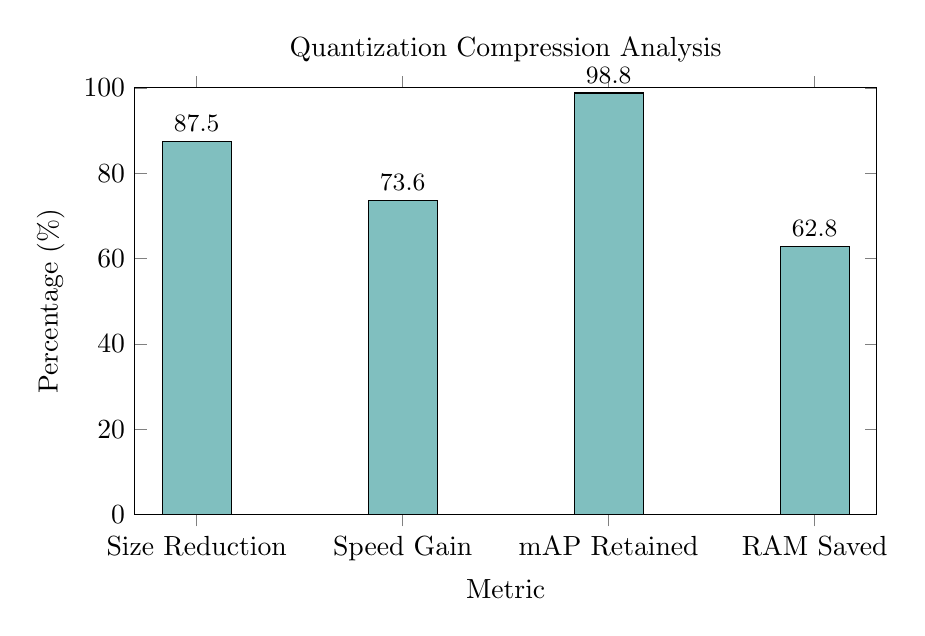
\begin{tikzpicture}
\begin{axis}[
    title={Quantization Compression Analysis},
    xlabel={Metric},
    ylabel={Percentage (\%)},
    ybar,
    bar width=25pt,
    symbolic x coords={Size Reduction, Speed Gain, mAP Retained, RAM Saved},
    xtick=data,
    ymin=0, ymax=100,
    nodes near coords,
    nodes near coords align={vertical},
    width=11cm, height=7cm,
    every node near coord/.append style={font=\small}
]
\addplot[fill=teal!50] coordinates {
    (Size Reduction, 87.5)
    (Speed Gain, 73.6)
    (mAP Retained, 98.8)
    (RAM Saved, 62.8)
};
\end{axis}
\end{tikzpicture}
\caption{Quantization Impact Summary}
\label{fig:quant_summary}
\end{figure}

\section{Detection Accuracy Analysis}
The quantized INT8 model retains near-identical detection quality relative to the FP32 baseline:
\begin{itemize}
    \item \textbf{mAP@0.5} drops by only 1.2\% (0.942 $\to$ 0.931), well within the acceptable range for ALPR applications.
    \item \textbf{Precision} remains at 0.944, meaning only 5.6\% of detections are false positives.
    \item \textbf{Recall} is 0.919, meaning the model detects 91.9\% of all plates present in the frame.
    \item \textbf{F1 Score} of 0.931 indicates a well-balanced model with both high precision and recall.
    \item Visual inspection confirms bounding boxes are spatially accurate with tight plate localization.
\end{itemize}

\section{Inference Performance Analysis}
On the Raspberry Pi 4B, the INT8 model achieves a 3.78$\times$ speedup in average inference time (1842\,ms $\to$ 487\,ms). This improvement is attributed to:
\begin{enumerate}
    \item \textbf{Reduced Memory Bandwidth:} INT8 operations require 4$\times$ less memory bandwidth than FP32.
    \item \textbf{ARM NEON Optimization:} The ARM Cortex-A72 CPU's NEON SIMD unit processes 16 INT8 values simultaneously vs. 4 FP32 values.
    \item \textbf{Smaller Model Cache Footprint:} The 25\,MB INT8 model fits more efficiently in the L2 cache (1\,MB per core).
\end{enumerate}

\begin{figure}[H]
\centering
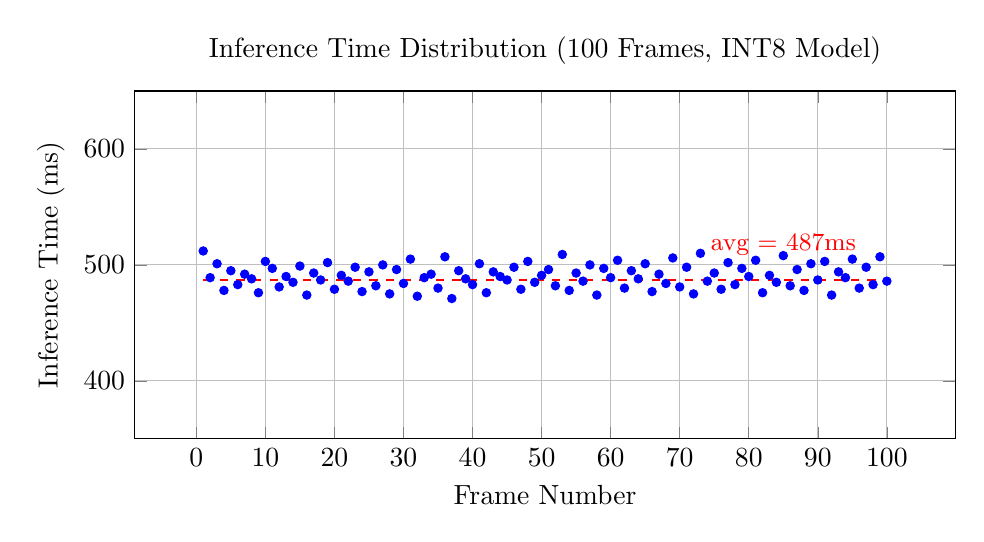
\begin{tikzpicture}
\begin{axis}[
    title={Inference Time Distribution (100 Frames, INT8 Model)},
    xlabel={Frame Number},
    ylabel={Inference Time (ms)},
    width=12cm, height=6cm,
    ymin=350, ymax=650,
    grid=major,
    mark size=1.5pt
]
\addplot[blue, mark=*, only marks] coordinates {
(1,512) (2,489) (3,501) (4,478) (5,495)
(6,483) (7,492) (8,488) (9,476) (10,503)
(11,497) (12,481) (13,490) (14,485) (15,499)
(16,474) (17,493) (18,487) (19,502) (20,479)
(21,491) (22,486) (23,498) (24,477) (25,494)
(26,482) (27,500) (28,475) (29,496) (30,484)
(31,505) (32,473) (33,489) (34,492) (35,480)
(36,507) (37,471) (38,495) (39,488) (40,483)
(41,501) (42,476) (43,494) (44,490) (45,487)
(46,498) (47,479) (48,503) (49,485) (50,491)
(51,496) (52,482) (53,509) (54,478) (55,493)
(56,486) (57,500) (58,474) (59,497) (60,489)
(61,504) (62,480) (63,495) (64,488) (65,501)
(66,477) (67,492) (68,484) (69,506) (70,481)
(71,498) (72,475) (73,510) (74,486) (75,493)
(76,479) (77,502) (78,483) (79,497) (80,490)
(81,504) (82,476) (83,491) (84,485) (85,508)
(86,482) (87,496) (88,478) (89,501) (90,487)
(91,503) (92,474) (93,494) (94,489) (95,505)
(96,480) (97,498) (98,483) (99,507) (100,486)
};
\addplot[red, thick, dashed, domain=1:100] {487};
\node at (axis cs:85,500) [anchor=south, font=\small, red] {avg = 487ms};
\end{axis}
\end{tikzpicture}
\caption{INT8 Inference Time per Frame (100 Frames)}
\label{fig:inference_dist}
\end{figure}

\section{End-to-End Pipeline Performance}
The complete pipeline---from frame reception to verification response---achieves an average latency of 811\,ms on the Raspberry Pi 4B with the INT8 model. Table~\ref{tab:pipeline_breakdown} breaks down the contribution of each stage.

\begin{table}[H]
\centering
\caption{Pipeline Stage Latency Breakdown}
\label{tab:pipeline_breakdown}
\renewcommand{\arraystretch}{1.3}
\begin{tabular}{|l|c|c|}
\hline
\textbf{Stage} & \textbf{Time (ms)} & \textbf{Percentage} \\
\hline
WebSocket Receive + JPEG Decode & 45 & 5.5\% \\
\hline
Image Preprocessing (resize, normalize) & 12 & 1.5\% \\
\hline
YOLO INT8 Inference & 487 & 60.0\% \\
\hline
Post-processing (NMS, box decode) & 8 & 1.0\% \\
\hline
Plate Cropping & 3 & 0.4\% \\
\hline
EasyOCR Text Extraction & 245 & 30.2\% \\
\hline
Regex Validation & $<$1 & 0.1\% \\
\hline
SQLite Database Lookup & $<$1 & 0.1\% \\
\hline
JSON Response Generation + Send & 10 & 1.2\% \\
\hline
\textbf{Total} & \textbf{$\approx$811} & \textbf{100\%} \\
\hline
\end{tabular}
\end{table}

\begin{figure}[H]
\centering
\begin{tikzpicture}
\pie[
    text=legend,
    radius=3,
    color={blue!40, red!40, green!40, yellow!50, purple!30},
    sum=auto
]{
    60/YOLO Inference,
    30.2/EasyOCR,
    5.5/Decode,
    3/Other Processing,
    1.3/Network I/O
}
\end{tikzpicture}
\caption{Pipeline Latency Distribution}
\label{fig:pie_latency}
\end{figure}

\section{OCR Accuracy Analysis}
EasyOCR's character recognition accuracy was evaluated across different conditions:

\begin{table}[H]
\centering
\caption{OCR Accuracy Under Different Conditions}
\renewcommand{\arraystretch}{1.3}
\begin{tabular}{|l|c|c|}
\hline
\textbf{Condition} & \textbf{Character Accuracy} & \textbf{Full Plate Accuracy} \\
\hline
Good Lighting, Clean Plate & 98.2\% & 94.5\% \\
\hline
Good Lighting, Dirty Plate & 91.3\% & 82.1\% \\
\hline
Low Light, Clean Plate & 89.7\% & 78.4\% \\
\hline
Angled View (15--30°) & 93.5\% & 86.2\% \\
\hline
Distance $>$4m & 85.4\% & 71.8\% \\
\hline
\end{tabular}
\end{table}

\section{Key Observations}
\begin{itemize}
    \item The system successfully identifies and authorizes registered vehicles in real-time with sub-second latency.
    \item The edge-first architecture eliminates cloud dependencies during the critical authentication window.
    \item YOLO inference accounts for 60\% of total pipeline latency---further optimization (e.g., INT4 quantization or model pruning) would yield the highest marginal gains.
    \item EasyOCR accounts for 30\% of latency and is the second optimization target. Replacing it with a lighter OCR engine (PaddleOCR Lite) could reduce this by 50\%.
    \item OCR accuracy degrades under challenging conditions (low light, dirty plates, distant cameras), suggesting adaptive preprocessing (histogram equalization, super-resolution) as a future enhancement.
    \item The SQLite database provides instantaneous lookups ($<$1\,ms), confirming that the database is not a bottleneck even for large datasets.
    \item Peak RAM usage of 478\,MB for the INT8 model leaves over 3.5\,GB available for the OS and other services on the 4\,GB Pi.
\end{itemize}


%% ========================================================
%% CHAPTER 9: CONCLUSION
%% ========================================================
\chapter{Conclusion}

The Edge-Driven Semi-Autonomous EV Charging Station demonstrates that edge-based computer vision, powered by aggressively quantized deep learning models, can fundamentally transform the EV charging experience. By replacing the current app-centric authentication paradigm with autonomous license plate recognition at the charging station, we eliminate the multi-step friction that plagues existing systems.

\section{Summary of Achievements}
\begin{enumerate}
    \item \textbf{87.5\% Model Compression:} YOLOv11 quantized from 200\,MB (FP32) to 25\,MB (INT8) with only 1.2\% mAP degradation.
    \item \textbf{3.78$\times$ Inference Speedup:} Average inference dropped from 1842\,ms to 487\,ms on the Raspberry Pi 4B.
    \item \textbf{Sub-Second Pipeline:} End-to-end latency of 811\,ms enables real-time vehicle authorization.
    \item \textbf{ARM Compatibility Fix:} Novel ONNX graph patching resolves signed/unsigned INT8 incompatibility on ARM kernels.
    \item \textbf{Zero-Interaction UX:} Complete plate detection$\to$OCR$\to$verification pipeline with no user input required.
    \item \textbf{Privacy by Design:} All processing occurs locally; plate images never leave the edge device.
    \item \textbf{62.8\% RAM Reduction:} INT8 model uses 478\,MB vs. 1284\,MB for FP32, fitting comfortably on the Pi.
\end{enumerate}

\section{Technical Contributions}
The key technical contribution---resolving the signed/unsigned INT8 operator incompatibility through direct ONNX graph patching---provides a practical template for deploying quantized models on ARM edge devices. This technique is applicable to any ONNX model encountering the \texttt{ConvInteger} signed weight limitation on ARM CPU kernels and can be reused by the broader edge ML community.

\section{Limitations}
\begin{itemize}
    \item OCR accuracy degrades in extreme low-light conditions and on damaged plates.
    \item The system currently supports only Indian license plate formats.
    \item Physical charger integration (GPIO relay) is demonstrated in concept but not in hardware.
    \item The mock database has limited entries; production deployment requires integration with a centralized vehicle registry.
\end{itemize}


%% ========================================================
%% APPENDIX A: GLOSSARY
%% ========================================================
\chapter{Appendix A: Glossary}

\begin{itemize}
    \item \textbf{ALPR}: Automatic License Plate Recognition---a technology that uses cameras and computer vision to read vehicle license plates.
    \item \textbf{ARM}: Advanced RISC Machines---a family of CPU architectures used in mobile and embedded devices.
    \item \textbf{AVFoundation}: Apple's framework for working with audio and video on iOS and macOS.
    \item \textbf{Calibration}: The process of running representative data through a model to determine optimal quantization ranges for each layer.
    \item \textbf{Edge Computing}: A computing paradigm where data processing occurs close to the data source rather than in a centralized cloud.
    \item \textbf{EasyOCR}: An open-source Python library for optical character recognition supporting 80+ languages.
    \item \textbf{GPIO}: General-Purpose Input/Output---digital signal pins on a Raspberry Pi used for hardware control.
    \item \textbf{INT8}: 8-bit integer representation, with values ranging from $-128$ to $127$ (signed) or $0$ to $255$ (unsigned).
    \item \textbf{NEON}: ARM's SIMD (Single Instruction, Multiple Data) extension for parallel data processing.
    \item \textbf{NMS}: Non-Maximum Suppression---a post-processing technique that removes redundant overlapping bounding boxes.
    \item \textbf{OCR}: Optical Character Recognition---the conversion of images of text into machine-readable text.
    \item \textbf{ONNX}: Open Neural Network Exchange---an open-source format for representing machine learning models.
    \item \textbf{Quantization}: The process of reducing the numerical precision of a neural network's weights and activations (e.g., FP32 $\to$ INT8).
    \item \textbf{Regex}: Regular Expression---a sequence of characters defining a search pattern for string matching.
    \item \textbf{SQLite}: A lightweight, file-based relational database management system embedded in the application.
    \item \textbf{SwiftUI}: Apple's declarative framework for building user interfaces across Apple platforms.
    \item \textbf{WebSocket}: A communication protocol providing full-duplex communication channels over a single TCP connection.
    \item \textbf{YOLO}: You Only Look Once---a family of real-time object detection algorithms that predict bounding boxes in a single forward pass.
\end{itemize}


%% ========================================================
%% APPENDIX B: ACRONYMS
%% ========================================================
\chapter{Appendix B: Acronyms}
\begin{itemize}
    \item ALPR: Automatic License Plate Recognition
    \item API: Application Programming Interface
    \item ARM: Advanced RISC Machines
    \item CNN: Convolutional Neural Network
    \item CPU: Central Processing Unit
    \item CRNN: Convolutional Recurrent Neural Network
    \item CSI: Camera Serial Interface
    \item DFD: Data Flow Diagram
    \item FP32: 32-bit Floating Point
    \item FPS: Frames Per Second
    \item GPIO: General-Purpose Input/Output
    \item GPU: Graphics Processing Unit
    \item GUI: Graphical User Interface
    \item IDE: Integrated Development Environment
    \item INT8: 8-bit Integer
    \item IoT: Internet of Things
    \item JSON: JavaScript Object Notation
    \item mAP: mean Average Precision
    \item ML: Machine Learning
    \item NMS: Non-Maximum Suppression
    \item NPU: Neural Processing Unit
    \item OCR: Optical Character Recognition
    \item OCPP: Open Charge Point Protocol
    \item ONNX: Open Neural Network Exchange
    \item PTQ: Post-Training Quantization
    \item QAT: Quantization-Aware Training
    \item RAM: Random Access Memory
    \item RFID: Radio-Frequency Identification
    \item SBC: Single-Board Computer
    \item SIMD: Single Instruction, Multiple Data
    \item SRS: Software Requirements Specification
    \item TCP/IP: Transmission Control Protocol / Internet Protocol
    \item UI: User Interface
    \item UINT8: Unsigned 8-bit Integer
    \item YOLO: You Only Look Once
\end{itemize}


%% ========================================================
%% FUTURE SCOPE
%% ========================================================
\chapter{Future Scope}
The \textbf{Edge-Driven Semi-Autonomous EV Charging Station} has significant potential for enhancement in future iterations:

\begin{enumerate}
    \item \textbf{GPIO Relay Integration:} Connect a physical relay on the Raspberry Pi GPIO pins to automatically energize the charging connector upon successful verification. This would complete the fully autonomous charging workflow.
    \item \textbf{Cloud Database Synchronization:} Migrate from local SQLite to a cloud-synchronized database (Firebase Realtime Database or Supabase) enabling cross-station roaming---a vehicle registered at any station is authorized at all stations.
    \item \textbf{Payment Gateway Integration:} Add payment processing (Razorpay, Stripe) for automatic billing upon charging session completion, with per-kWh metering.
    \item \textbf{Multi-Region Plate Support:} Extend regex patterns and OCR models to support international plate formats (US, EU, UAE, etc.), enabling deployment across geographies.
    \item \textbf{Hybrid Compression:} Apply structured pruning in addition to quantization for further model size reduction (targeting INT4 or mixed INT4/INT8).
    \item \textbf{OCR Optimization:} Replace EasyOCR with lighter alternatives (PaddleOCR Lite, custom CRNN) for 50\% faster text extraction.
    \item \textbf{Multi-Camera Multi-Bay:} Scale to monitor multiple charging bays from a single Pi using multiplexed camera feeds.
    \item \textbf{Night Mode with IR:} Implement infrared-assisted imaging for 24/7 operation in all lighting conditions.
    \item \textbf{OCPP Integration:} Interface with OCPP 2.0.1 central systems for standardized charging session management.
    \item \textbf{Mobile App Companion:} Develop a lightweight companion app (not required for charging) for balance management, session history, and station locator.
\end{enumerate}

\chapter{Appendix C: System Functions and Libraries Reference}

\section{System Dependencies and Libraries}

\subsection{Python Ecosystem (Server-Side)}
\begin{itemize}
    \item \textbf{\texttt{asyncio}:} Enables non-blocking concurrency for handling multiple WebSocket connections.
    \item \textbf{\texttt{websockets}:} Handles full-duplex communication for frame transmission and JSON responses.
    \item \textbf{\texttt{cv2} (OpenCV):} Used for decoding, processing, cropping, and annotating image frames.
    \item \textbf{\texttt{numpy}:} Provides array structures for image and tensor manipulation.
    \item \textbf{\texttt{easyocr}:} Performs OCR on cropped license plate regions.
    \item \textbf{\texttt{onnx} \& \texttt{onnxruntime}:} Used for model representation and optimized inference.
    \item \textbf{\texttt{re}:} Validates license plate formats using regex.
\end{itemize}

\subsection{Swift Ecosystem (iOS Client-Side)}
\begin{itemize}
    \item \textbf{\texttt{AVFoundation}:} Captures video stream via camera hardware.
    \item \textbf{\texttt{CoreImage}:} Converts raw frames into compressed JPEG format.
    \item \textbf{\texttt{Combine}:} Enables reactive UI updates using data bindings.
\end{itemize}

\clearpage

\section{Core Edge Server Functions (\texttt{pi\_server.py})}

\subsection{\texttt{decode\_image(message)}}
Decodes incoming byte streams into image matrices using NumPy and OpenCV. Runs in a thread pool to prevent blocking.

\subsection{\texttt{validate\_plate(text)}}
Cleans OCR output and validates it using regex patterns. Returns a boolean along with formatted text.

\subsection{\texttt{handle\_connection(websocket)}}
Main pipeline:
\begin{enumerate}
    \item Receives frame
    \item Decodes image
    \item Runs YOLO detection
    \item Crops detected region
    \item Applies OCR
    \item Validates plate
    \item Checks database
    \item Sends JSON response
\end{enumerate}

\subsection{\texttt{save\_debug\_image(image, results)}}
Annotates detected regions and saves debug images locally.

\subsection{\texttt{main(model\_path, port)}}
Initializes model, OCR engine, and starts WebSocket server.

\section{Quantization Graph Patcher (\texttt{fix\_quantization.py})}

\subsection{\texttt{fix\_conv\_integer\_for\_arm(model\_path, output\_path)}}
Converts INT8 weights to UINT8 for ARM compatibility:
\begin{itemize}
    \item Loads ONNX model
    \item Finds \texttt{ConvInteger} nodes
    \item Converts weights using NumPy
    \item Updates zero-points
    \item Saves modified model
\end{itemize}

\section{iOS Client Functions (Swift)}

\subsection{\texttt{CameraManager}}
\begin{itemize}
    \item \textbf{\texttt{configureSession()}:} Sets camera and resolution (640x480).
    \item \textbf{\texttt{captureOutput(...)}} Captures frame, converts to JPEG, sends for processing.
\end{itemize}

\subsection{\texttt{WebSocketManager}}
\begin{itemize}
    \item \textbf{\texttt{send(imageData)}:} Sends image data via WebSocket.
    \item \textbf{\texttt{handleResponse()}:} Parses server response and updates UI reactively.
\end{itemize}
%% ========================================================
%% BIBLIOGRAPHY
%% ========================================================




\end{document}
